% Options for packages loaded elsewhere
\PassOptionsToPackage{unicode}{hyperref}
\PassOptionsToPackage{hyphens}{url}
%
\documentclass[
  oneside]{book}
\usepackage{amsmath,amssymb}
\usepackage{iftex}
\ifPDFTeX
  \usepackage[T1]{fontenc}
  \usepackage[utf8]{inputenc}
  \usepackage{textcomp} % provide euro and other symbols
\else % if luatex or xetex
  \usepackage{unicode-math} % this also loads fontspec
  \defaultfontfeatures{Scale=MatchLowercase}
  \defaultfontfeatures[\rmfamily]{Ligatures=TeX,Scale=1}
\fi
\usepackage{lmodern}
\ifPDFTeX\else
  % xetex/luatex font selection
\fi
% Use upquote if available, for straight quotes in verbatim environments
\IfFileExists{upquote.sty}{\usepackage{upquote}}{}
\IfFileExists{microtype.sty}{% use microtype if available
  \usepackage[]{microtype}
  \UseMicrotypeSet[protrusion]{basicmath} % disable protrusion for tt fonts
}{}
\makeatletter
\@ifundefined{KOMAClassName}{% if non-KOMA class
  \IfFileExists{parskip.sty}{%
    \usepackage{parskip}
  }{% else
    \setlength{\parindent}{0pt}
    \setlength{\parskip}{6pt plus 2pt minus 1pt}}
}{% if KOMA class
  \KOMAoptions{parskip=half}}
\makeatother
\usepackage{xcolor}
\usepackage[left=3cm,right=3cm,top=3cm,bottom=3cm]{geometry}
\usepackage{color}
\usepackage{fancyvrb}
\newcommand{\VerbBar}{|}
\newcommand{\VERB}{\Verb[commandchars=\\\{\}]}
\DefineVerbatimEnvironment{Highlighting}{Verbatim}{commandchars=\\\{\}}
% Add ',fontsize=\small' for more characters per line
\usepackage{framed}
\definecolor{shadecolor}{RGB}{248,248,248}
\newenvironment{Shaded}{\begin{snugshade}}{\end{snugshade}}
\newcommand{\AlertTok}[1]{\textcolor[rgb]{0.94,0.16,0.16}{#1}}
\newcommand{\AnnotationTok}[1]{\textcolor[rgb]{0.56,0.35,0.01}{\textbf{\textit{#1}}}}
\newcommand{\AttributeTok}[1]{\textcolor[rgb]{0.13,0.29,0.53}{#1}}
\newcommand{\BaseNTok}[1]{\textcolor[rgb]{0.00,0.00,0.81}{#1}}
\newcommand{\BuiltInTok}[1]{#1}
\newcommand{\CharTok}[1]{\textcolor[rgb]{0.31,0.60,0.02}{#1}}
\newcommand{\CommentTok}[1]{\textcolor[rgb]{0.56,0.35,0.01}{\textit{#1}}}
\newcommand{\CommentVarTok}[1]{\textcolor[rgb]{0.56,0.35,0.01}{\textbf{\textit{#1}}}}
\newcommand{\ConstantTok}[1]{\textcolor[rgb]{0.56,0.35,0.01}{#1}}
\newcommand{\ControlFlowTok}[1]{\textcolor[rgb]{0.13,0.29,0.53}{\textbf{#1}}}
\newcommand{\DataTypeTok}[1]{\textcolor[rgb]{0.13,0.29,0.53}{#1}}
\newcommand{\DecValTok}[1]{\textcolor[rgb]{0.00,0.00,0.81}{#1}}
\newcommand{\DocumentationTok}[1]{\textcolor[rgb]{0.56,0.35,0.01}{\textbf{\textit{#1}}}}
\newcommand{\ErrorTok}[1]{\textcolor[rgb]{0.64,0.00,0.00}{\textbf{#1}}}
\newcommand{\ExtensionTok}[1]{#1}
\newcommand{\FloatTok}[1]{\textcolor[rgb]{0.00,0.00,0.81}{#1}}
\newcommand{\FunctionTok}[1]{\textcolor[rgb]{0.13,0.29,0.53}{\textbf{#1}}}
\newcommand{\ImportTok}[1]{#1}
\newcommand{\InformationTok}[1]{\textcolor[rgb]{0.56,0.35,0.01}{\textbf{\textit{#1}}}}
\newcommand{\KeywordTok}[1]{\textcolor[rgb]{0.13,0.29,0.53}{\textbf{#1}}}
\newcommand{\NormalTok}[1]{#1}
\newcommand{\OperatorTok}[1]{\textcolor[rgb]{0.81,0.36,0.00}{\textbf{#1}}}
\newcommand{\OtherTok}[1]{\textcolor[rgb]{0.56,0.35,0.01}{#1}}
\newcommand{\PreprocessorTok}[1]{\textcolor[rgb]{0.56,0.35,0.01}{\textit{#1}}}
\newcommand{\RegionMarkerTok}[1]{#1}
\newcommand{\SpecialCharTok}[1]{\textcolor[rgb]{0.81,0.36,0.00}{\textbf{#1}}}
\newcommand{\SpecialStringTok}[1]{\textcolor[rgb]{0.31,0.60,0.02}{#1}}
\newcommand{\StringTok}[1]{\textcolor[rgb]{0.31,0.60,0.02}{#1}}
\newcommand{\VariableTok}[1]{\textcolor[rgb]{0.00,0.00,0.00}{#1}}
\newcommand{\VerbatimStringTok}[1]{\textcolor[rgb]{0.31,0.60,0.02}{#1}}
\newcommand{\WarningTok}[1]{\textcolor[rgb]{0.56,0.35,0.01}{\textbf{\textit{#1}}}}
\usepackage{longtable,booktabs,array}
\usepackage{calc} % for calculating minipage widths
% Correct order of tables after \paragraph or \subparagraph
\usepackage{etoolbox}
\makeatletter
\patchcmd\longtable{\par}{\if@noskipsec\mbox{}\fi\par}{}{}
\makeatother
% Allow footnotes in longtable head/foot
\IfFileExists{footnotehyper.sty}{\usepackage{footnotehyper}}{\usepackage{footnote}}
\makesavenoteenv{longtable}
\usepackage{graphicx}
\makeatletter
\def\maxwidth{\ifdim\Gin@nat@width>\linewidth\linewidth\else\Gin@nat@width\fi}
\def\maxheight{\ifdim\Gin@nat@height>\textheight\textheight\else\Gin@nat@height\fi}
\makeatother
% Scale images if necessary, so that they will not overflow the page
% margins by default, and it is still possible to overwrite the defaults
% using explicit options in \includegraphics[width, height, ...]{}
\setkeys{Gin}{width=\maxwidth,height=\maxheight,keepaspectratio}
% Set default figure placement to htbp
\makeatletter
\def\fps@figure{htbp}
\makeatother
\setlength{\emergencystretch}{3em} % prevent overfull lines
\providecommand{\tightlist}{%
  \setlength{\itemsep}{0pt}\setlength{\parskip}{0pt}}
\setcounter{secnumdepth}{5}
\usepackage{amsthm}
\usepackage{float}
\usepackage{rotating, graphicx}
\usepackage{multirow}
\usepackage{tabularx}

% new command for pretty oversets with \sim
\newcommand\simcal[1]{\stackrel{\sim}{\smash{\mathcal{#1}}\rule{0pt}{0.5ex}}}

\newcommand{\comma}{,\,}

\floatplacement{figure}{H}

\PassOptionsToPackage{table}{xcolor}

\usepackage{tcolorbox}

\definecolor{kcblue}{HTML}{D7DDEF}
\definecolor{kcdarkblue}{HTML}{2B4E70}

\makeatletter
\def\thm@space@setup{%
  \thm@preskip=8pt plus 2pt minus 4pt
  \thm@postskip=\thm@preskip
}
\makeatother

% \makeatletter % undo the wrong changes made by mathspec
% \let\RequirePackage\original@RequirePackage
% \let\usepackage\RequirePackage
% \makeatother

\newenvironment{rmdknit}
    {\begin{center}
    \begin{tabular}{|p{0.9\textwidth}|}
    \hline\\
    }
    {
    \\\\\hline
    \end{tabular}
    \end{center}
    }

\newenvironment{rmdnote}
    {\begin{center}
    \begin{tabular}{|p{0.9\textwidth}|}
    \hline\\
    }
    {
    \\\\\hline
    \end{tabular}
    \end{center}
    }

\newtcolorbox[auto counter, number within=section]{keyconcepts}[2][]{%
colback=kcblue,colframe=kcdarkblue,fonttitle=\bfseries, title=Key Concept~#2, after title={\newline #1}, beforeafter skip=15pt}

\ifLuaTeX
  \usepackage{selnolig}  % disable illegal ligatures
\fi
\usepackage[]{natbib}
\bibliographystyle{apalike}
\usepackage{bookmark}
\IfFileExists{xurl.sty}{\usepackage{xurl}}{} % add URL line breaks if available
\urlstyle{same}
\hypersetup{
  pdftitle={Analisis Cluster dengan R: Panduan Lengkap untuk Pemula},
  pdfauthor={Deden Istiawan},
  hidelinks,
  pdfcreator={LaTeX via pandoc}}

\title{Analisis Cluster dengan R: Panduan Lengkap untuk Pemula}
\author{Deden Istiawan}
\date{2025-01-03}

\begin{document}
\maketitle

{
\setcounter{tocdepth}{1}
\tableofcontents
}
\chapter*{Kata Pengantar}\label{kata-pengantar}
\addcontentsline{toc}{chapter}{Kata Pengantar}

Rekayasa Perangkat Lunak
Fakultas Sains dan Teknologi Institut Teknologi Statistika dan
Bisnis Muhammadiyah Semarang, Indonesia
\href{mailto:deden.istiawan@itesa.ac.id}{\nolinkurl{deden.istiawan@itesa.ac.id}}.
Last updated on Friday, January 03, 2025.

Analisis \emph{cluster} merupakan teknik yang sangat penting dalam bidang data
science, karena kemampuannya untuk mengelompokkan data berdasarkan
kesamaan karakteristik. Dengan mengelompokkan objek atau data, analisis
cluster membantu mengidentifikasi pola yang mungkin tidak terlihat
secara langsung dalam data mentah. Hal ini sangat berguna di berbagai
bidang, seperti pemasaran, biologi, dan pengenalan pola, di mana
pemahaman yang lebih dalam tentang struktur data dapat memberikan
wawasan yang berharga \citep{kaufman:clustering1990}.

Salah satu manfaat utama dari analisis cluster adalah segmentasi pasar.
Dalam dunia bisnis, perusahaan dapat menggunakan teknik ini untuk
mengelompokkan pelanggan berdasarkan perilaku atau karakteristik
tertentu. Dengan memahami segmen-segmen ini, perusahaan dapat merancang
strategi pemasaran yang lebih efektif dan personalisasi produk untuk
memenuhi kebutuhan spesifik dari setiap kelompok. Selain itu, analisis
cluster juga memungkinkan pengelompokan data yang besar menjadi lebih
mudah dipahami dan diinterpretasikan, sehingga memfasilitasi pengambilan
keputusan yang lebih baik \citep{han2012mining}.

Dalam konteks machine learning, analisis cluster sering digunakan
sebagai metode unsupervised learning. Ini berarti bahwa algoritma
clustering dapat menemukan struktur dalam data tanpa memerlukan label
atau kategori sebelumnya. Hal ini sangat berguna ketika menghadapi
dataset yang tidak terstruktur dan kompleks, di mana tujuan utamanya
adalah untuk mengeksplorasi dan mendapatkan wawasan awal tentang data
tersebut \citep{jain2010}.

Secara keseluruhan, analisis cluster tidak hanya membantu dalam
pengelompokan data tetapi juga berfungsi sebagai alat eksplorasi yang
kuat dalam memahami hubungan dan pola dalam dataset. Dengan demikian,
penerapan analisis cluster dapat meningkatkan kualitas analisis data dan
mendukung pengambilan keputusan berbasis data yang lebih baik di
berbagai sektor industri .

\subsubsection*{Ucapan Terimakasih}\label{ucapan-terimakasih}
\addcontentsline{toc}{subsubsection}{Ucapan Terimakasih}

Saya ingin mengucapkan terima kasih kepada keluarga, teman, dan rekan kerja yang telah mendukung saya dalam menyelesaikan buku ini. Terima kasih atas cinta, dukungan, dan motivasi yang telah Anda berikan

\chapter{Pendahuluan}\label{pd}

\begin{quote}
``Why is that when one man builds a wall, the next needs to to know
what's on the other side?''

-- Tyrion Lannister-Game of Thrones
\end{quote}

\texttt{R} adalah bahasa pemrograman dan perangkat lunak yang
dirancang khusus untuk keperluan analisis data, pengolahan statistik,
dan visualisasi. Bahasa ini menawarkan fleksibilitas untuk menulis kode
guna menjalankan berbagai metode analisis statistik, mulai dari
deskriptif hingga prediktif. Sebagai perangkat lunak, R menyediakan
lingkungan interaktif untuk eksplorasi data, pengolahan, serta pembuatan
laporan yang informatif.

\texttt{R} pertama kali dikembangkan pada awal 1990-an oleh Ross
Ihaka dan Robert Gentleman di University of Auckland, Selandia Baru.
Proyek ini terinspirasi oleh bahasa pemrograman S yang dikembangkan oleh
John Chambers di Bell Laboratories. Pada tahun 1995, \texttt{R}
dirilis sebagai perangkat lunak open source, sehingga memungkinkan
pengembang di seluruh dunia untuk berkontribusi dalam pengembangannya.

Sejak itu, \texttt{R} berkembang pesat dengan ribuan paket yang
tersedia di \href{https://cran.r-project.org/}{CRAN} (Comprehensive R Archive
Network) serta repositori lainnya. Dukungan komunitas dan kontribusi
aktif dari pengembang di seluruh dunia telah menjadikan \texttt{R}
sebagai bahasa yang terus berevolusi untuk memenuhi kebutuhan analisis
data modern.

\texttt{R} memiliki salah satu komunitas pengguna paling aktif di
dunia. Komunitas ini terdiri dari akademisi, peneliti, praktisi
industri, hingga pengembang perangkat lunak. Forum diskusi seperti
RStudio Community, Stack Overflow, dan mailing list \texttt{R}
membantu pengguna menyelesaikan masalah serta berbagi ide.

Ekosistem \texttt{R} terus berkembang dengan adanya \textbf{RStudio}
sebagai Integrated Development Environment (IDE) yang populer, serta
berbagai konferensi seperti useR! yang mempertemukan pengguna R dari
seluruh dunia. Selain itu, repositori paket seperti CRAN dan
Bioconductor menyediakan ribuan alat tambahan untuk berbagai kebutuhan
analisis.Dukungan komunitas yang besar, dokumentasi yang melimpah, dan
ketersediaan sumber daya membuat \texttt{R} menjadi alat yang mudah
diakses oleh pemula sekaligus sangat berguna bagi pengguna tingkat
lanjut.

\texttt{R} adalah perangkat lunak open source yang sepenuhnya
gratis untuk digunakan oleh siapa saja. Tidak seperti beberapa perangkat
lunak statistik lainnya yang membutuhkan biaya lisensi mahal,
\texttt{R} memberikan fleksibilitas bagi pengguna untuk
mendownload, menginstal, dan memodifikasi kode sumbernya tanpa batasan.
Hal ini menjadikan \texttt{R} pilihan ideal bagi akademisi,
peneliti, dan praktisi yang ingin menghemat biaya sekaligus mendapatkan
alat analisis data yang andal.

\texttt{R} dirancang khusus untuk analisis statistik dan pengolahan
data, dengan dukungan bawaan untuk berbagai metode analisis, mulai dari
deskriptif hingga prediktif. Kemampuan ini diperkuat dengan pustaka
visualisasi yang sangat kaya seperti \texttt{ggplot2}, \texttt{lattice}, dan \texttt{plotly},
yang memungkinkan pengguna membuat grafik berkualitas tinggi.
\texttt{R} tidak hanya membantu menganalisis data tetapi juga
memvisualisasikannya dengan cara yang interaktif dan estetis, sehingga
dapat menggali wawasan yang lebih dalam.

Ekosistem \texttt{R} sangat kaya dengan ribuan pustaka atau paket
tambahan yang tersedia di \href{https://cran.r-project.org/}{CRAN}
(Comprehensive R Archive Network), Bioconductor, dan repositori lainnya.
Paket-paket ini mencakup berbagai bidang aplikasi, seperti analisis
genetik, analisis spasial, pengolahan teks, hingga machine learning.
Dengan pustaka ini, pengguna dapat dengan mudah memperluas fungsi
\texttt{R} untuk memenuhi kebutuhan spesifik mereka tanpa harus
menulis kode dari awal.

\texttt{R} dapat diintegrasikan dengan berbagai bahasa pemrograman
lain, seperti Python, C++, Java, dan SQL. Kompatibilitas ini
memungkinkan pengguna untuk menggabungkan kekuatan masing-masing bahasa
dalam satu proyek. Misalnya, pengguna dapat memanfaatkan Python untuk
preprocessing data skala besar, kemudian menggunakan \texttt{R}
untuk analisis statistik mendalam dan visualisasi. Selain itu,
\texttt{R} juga mendukung integrasi dengan berbagai perangkat lunak
lain seperti Excel, Tableau, dan Power BI, membuatnya menjadi bagian
penting dalam alur kerja data modern.

\texttt{R} telah menjadi alat yang sangat populer di berbagai
bidang, berkat fleksibilitasnya dalam menangani analisis data. Beberapa
bidang utama yang banyak memanfaatkan \texttt{R} antara lain:

\begin{itemize}
\item
  \textbf{Statistik:} \texttt{R} digunakan untuk berbagai jenis
  analisis statistik, seperti uji hipotesis, analisis regresi, dan
  analisis multivariat.
\item
  \textbf{Ilmu Data:} \texttt{R} digunakan untuk eksplorasi data,
  pembuatan model prediktif, dan pengolahan data besar.
\item
  \textbf{Biologi dan Bioinformatika:} Paket seperti \texttt{Bioconductor}
  memungkinkan analisis data genomik dan proteomik.
\item
  \textbf{Ekonomi dan Keuangan:} \texttt{R} digunakan untuk analisis
  time series, pemodelan risiko, dan optimasi portofolio.
\item
  \textbf{Ilmu Sosial}: \texttt{R} membantu dalam analisis survei,
  data panel, dan analisis konten.
\end{itemize}

\texttt{R} dirancang khusus untuk analisis statistik, membuatnya
menjadi salah satu alat terbaik untuk keperluan ini. Selain itu,
\texttt{R} menyediakan banyak metode untuk data mining, seperti
clustering, classification, dan association rule mining. Dukungan
pustaka seperti caret untuk pembelajaran mesin dan tm untuk analisis
teks menjadikan \texttt{R} alat yang sangat andal dalam penggalian
data (data mining) dan pengolahan data tidak terstruktur.

Selain itu, paket \texttt{bookdown} menjadi alat utama dalam proyek ini. Paket
ini berbasis rmarkdown dan memberikan kemudahan untuk membuat dokumen
yang menarik, seperti halaman web interaktif, e-book, dan laporan dalam
format PDF. Dengan fitur yang memungkinkan integrasi antara teks, kode,
dan hasil analisis, bookdown sangat cocok digunakan untuk pembelajaran
dan dokumentasi ilmiah.

Dengan menggunakan alat ini, kami menyusun sebuah buku berjudul
\emph{Analisis Cluster dengan R: Panduan Lengkap untuk Pemula}. Buku ini
dirancang sebagai panduan interaktif yang menggabungkan teori, kode, dan
hasil analisis dalam satu kesatuan. Tujuannya adalah menyediakan bahan
belajar elektronik yang dapat diakses di berbagai platform, sehingga
pembaca dapat memahami teori sekaligus mempraktikkan analisis data
secara langsung. Buku ini diharapkan menjadi panduan lengkap bagi pemula
untuk mempelajari analisis cluster dengan pendekatan yang mudah dipahami
dan terstruktur.

Setiap bab dalam buku ini dilengkapi dengan latihan pemrograman
interaktif menggunakan \texttt{R}. Latihan-latihan ini dirancang
untuk melengkapi contoh kode yang menunjukkan penerapan teknik-teknik
yang dibahas. Latihan dibuat dengan menggunakan \href{https://github.com/datacamp/datacamp-light}{DataCamp light
widget} yang terhubung
langsung ke sesi \texttt{R} yang dikelola oleh server DataCamp.

Melalui pendekatan ini, pembaca dapat langsung mencoba dan bereksperimen
dengan latihan yang disediakan, sehingga pemahaman mereka terhadap
metode yang dipelajari dapat lebih mendalam. Kami berharap metode ini
dapat memberikan pengalaman belajar yang menyeluruh dan menarik,
terutama bagi pembaca yang ingin mempelajari analisis cluster
menggunakan \texttt{R} secara praktis.

Widget ini terdiri dari dua tab. Tab pertama, \texttt{script.R},
berfungsi seperti file dengan format \texttt{.R}, yang umum
digunakan untuk menyimpan kode \texttt{R}. Baris yang diawali
dengan tanda \# merupakan komentar, yang tidak dihitung sebagai kode
oleh \texttt{R}. Tab \texttt{script.R} ini berfungsi seperti lembar
latihan, di mana Anda dapat menuliskan solusi Anda. Setelah menulis
kode, Anda bisa menekan tombol \emph{Run} untuk menjalankannya. Sistem akan
menguji kebenaran solusi yang Anda buat dan memberi tahu apakah solusi
tersebut benar. Jika salah, Anda akan mendapatkan umpan balik berupa
saran atau petunjuk perbaikan.

Tab kedua, \texttt{R Console}, adalah konsol \texttt{R} yang
sepenuhnya berfungsi, yang memungkinkan Anda mencoba solusi terlebih
dahulu sebelum mengirimkannya. Anda juga bisa mengirimkan hampir semua
kode R ke konsol untuk bereksperimen dan mengeksplorasi lebih lanjut.
Cukup ketikkan perintah dan tekan \emph{Enter} untuk menjalankannya.

Pada konsol, Anda akan melihat simbol \textgreater{} di panel kanan
(konsol). Simbol ini disebut ``prompt'' dan menandakan bahwa pengguna
dapat mulai memasukkan kode untuk dijalankan. Agar tidak membingungkan,
simbol ini tidak akan ditampilkan di buku ini. Output yang dihasilkan
oleh kode \texttt{R} akan diberi komentar dengan \#\textgreater{}.

Biasanya, kami menampilkan kode \texttt{R} bersama dengan output
yang dihasilkan dalam satu potongan kode. Sebagai contoh, perhatikan
baris kode berikut yang ditampilkan dalam potongan di bawah ini. Kode
ini memberi perintah kepada \texttt{R} untuk menghitung jumlah
paket yang tersedia di CRAN. Potongan kode tersebut diikuti oleh output
yang dihasilkan.

\begin{Shaded}
\begin{Highlighting}[]
\CommentTok{\# Cek jumlah paket R yang tersedia di CRAN}
\FunctionTok{nrow}\NormalTok{(}\FunctionTok{available.packages}\NormalTok{(}\AttributeTok{repos =} \StringTok{"http://cran.us.r{-}project.org"}\NormalTok{))}
\CommentTok{\#\textgreater{} [1] 21834}
\end{Highlighting}
\end{Shaded}

Setiap potongan kode dilengkapi dengan tombol di sisi kanan yang
memungkinkan Anda menyalin kode ke clipboard. Fitur ini mempermudah
pekerjaan dengan segmen kode yang lebih besar, baik di versi
R/\emph{RStudio} Anda maupun di widget-widget yang ada di sepanjang
buku ini. Pada widget di atas, Anda bisa mengklik tab
\texttt{R Console} dan mengetikkan perintah
\texttt{nrow(available.packages(repos\ =\ "http://cran.us.r-project.org"))}
(perintah dari potongan kode di atas), lalu menjalankannya dengan
menekan tombol \emph{Enter} pada keyboard Anda.

Setiap potongan kode dilengkapi dengan tombol di sisi kanan luar yang
memungkinkan Anda menyalin kode ke clipboard Anda. Ini membuat pekerjaan
dengan segmen kode yang lebih besar menjadi lebih nyaman, baik di versi
R/\emph{RStudio} Anda maupun di widget-widget yang disajikan di
sepanjang buku ini. Pada widget di atas, Anda dapat mengklik tab
\texttt{R Console} Console dan mengetikkan
\texttt{nrow(available.packages(repos\ =\ "http://cran.us.r-project.org"))}
(perintah dari potongan kode di atas) dan menjalankannya dengan menekan
tombol \emph{Enter} pada keyboard Anda. \footnote{Sesi \texttt{R} akan diinisialisasi dengan mengklik
  widget. Proses ini mungkin memakan waktu beberapa detik. Cukup
  tunggu hingga indikator di samping tombol \emph{Run} berubah menjadi
  hijau.}

\section{Kolofon}\label{kolofon}

Buku ini ditulis menggunakan \href{http://bookdown.org/}{bookdown} di dalam
\href{http://www.rstudio.com/ide/}{RStudio}. Seluruh kode sumbernya dapat
diakses di \href{https://github.com/dedenistiawan/ClustR}{GitHub}.

\begin{verbatim}
#> - Session info ---------------------------------------------------------------
#>  setting  value
#>  version  R version 4.4.0 (2024-04-24 ucrt)
#>  os       Windows 11 x64 (build 22631)
#>  system   x86_64, mingw32
#>  ui       RTerm
#>  language (EN)
#>  collate  English_Indonesia.utf8
#>  ctype    English_Indonesia.utf8
#>  tz       Asia/Jakarta
#>  date     2025-01-03
#>  pandoc   3.2 @ C:/Program Files/RStudio/resources/app/bin/quarto/bin/tools/ (via rmarkdown)
#> 
#> - Packages -------------------------------------------------------------------
#>  package     * version date (UTC) lib source
#>  bookdown      0.39    2024-04-15 [1] CRAN (R 4.4.0)
#>  cli           3.6.2   2023-12-11 [1] CRAN (R 4.4.0)
#>  digest        0.6.35  2024-03-11 [1] CRAN (R 4.4.0)
#>  evaluate      1.0.1   2024-10-10 [1] CRAN (R 4.4.2)
#>  fastmap       1.2.0   2024-05-15 [1] CRAN (R 4.4.0)
#>  htmltools     0.5.8.1 2024-04-04 [1] CRAN (R 4.4.0)
#>  knitr         1.47    2024-05-29 [1] CRAN (R 4.4.0)
#>  rlang         1.1.4   2024-06-04 [1] CRAN (R 4.4.0)
#>  rmarkdown     2.27    2024-05-17 [1] CRAN (R 4.4.0)
#>  rstudioapi    0.16.0  2024-03-24 [1] CRAN (R 4.4.0)
#>  sessioninfo   1.2.2   2021-12-06 [1] CRAN (R 4.4.2)
#>  tinytex       0.51    2024-05-06 [1] CRAN (R 4.4.0)
#>  xfun          0.49    2024-10-31 [1] CRAN (R 4.4.1)
#>  yaml          2.3.8   2023-12-11 [1] CRAN (R 4.4.0)
#> 
#>  [1] C:/Users/Deden/AppData/Local/R/win-library/4.4
#>  [2] C:/Program Files/R/R-4.4.0/library
#> 
#> ------------------------------------------------------------------------------
\end{verbatim}

\section{Pengenalan Singkat R and RStudio}\label{pengenalan-singkat-r-and-rstudio}

\subsection*{Instalasi R dan RStudio}\label{instalasi-r-dan-rstudio}
\addcontentsline{toc}{subsection}{Instalasi R dan RStudio}

Untuk memulai menggunakan \texttt{R}, langkah pertama adalah
menginstal perangkat lunaknya. Berikut langkah-langkah instalasinya:

\begin{enumerate}
\def\labelenumi{\arabic{enumi}.}
\item
  Buka situs resmi CRAN (Comprehensive R Archive Network) di
  \url{https://cran.r-project.org}.
\item
  Pilih sistem operasi yang digunakan (Windows, macOS, atau Linux).
\item
  Unduh file instalasi dan ikuti instruksi instalasinya. Unduh dan
  Instal RStudio
\end{enumerate}

Setelah \texttt{R} terinstal, unduh RStudio, sebuah Integrated
Development Environment (IDE) untuk \texttt{R}, dari
\url{https://www.rstudio.com}. Pilih versi gratis (RStudio Desktop) dan
instal sesuai dengan sistem operasi Anda.

RStudio adalah IDE yang dirancang khusus untuk mempermudah penggunaan
\texttt{R}. Dibandingkan dengan antarmuka dasar \texttt{R},
RStudio menawarkan pengalaman pengguna yang lebih nyaman melalui
fitur-fitur berikut:

\begin{itemize}
\item
  \textbf{Script Editor}: Memungkinkan penulisan dan pengelolaan skrip
  dengan mudah.
\item
  \textbf{Console}: Tempat menjalankan perintah \texttt{R} secara
  langsung.
\item
  \textbf{Environment Pane}: Menampilkan variabel, data, dan objek yang
  sedang aktif.
\item
  \textbf{Plots Pane}: Menampilkan hasil visualisasi seperti grafik dan
  plot.
\item
  \textbf{Packages Pane}: Memudahkan instalasi dan pengelolaan pustaka.
\end{itemize}

\begin{figure}[h]

{\centering 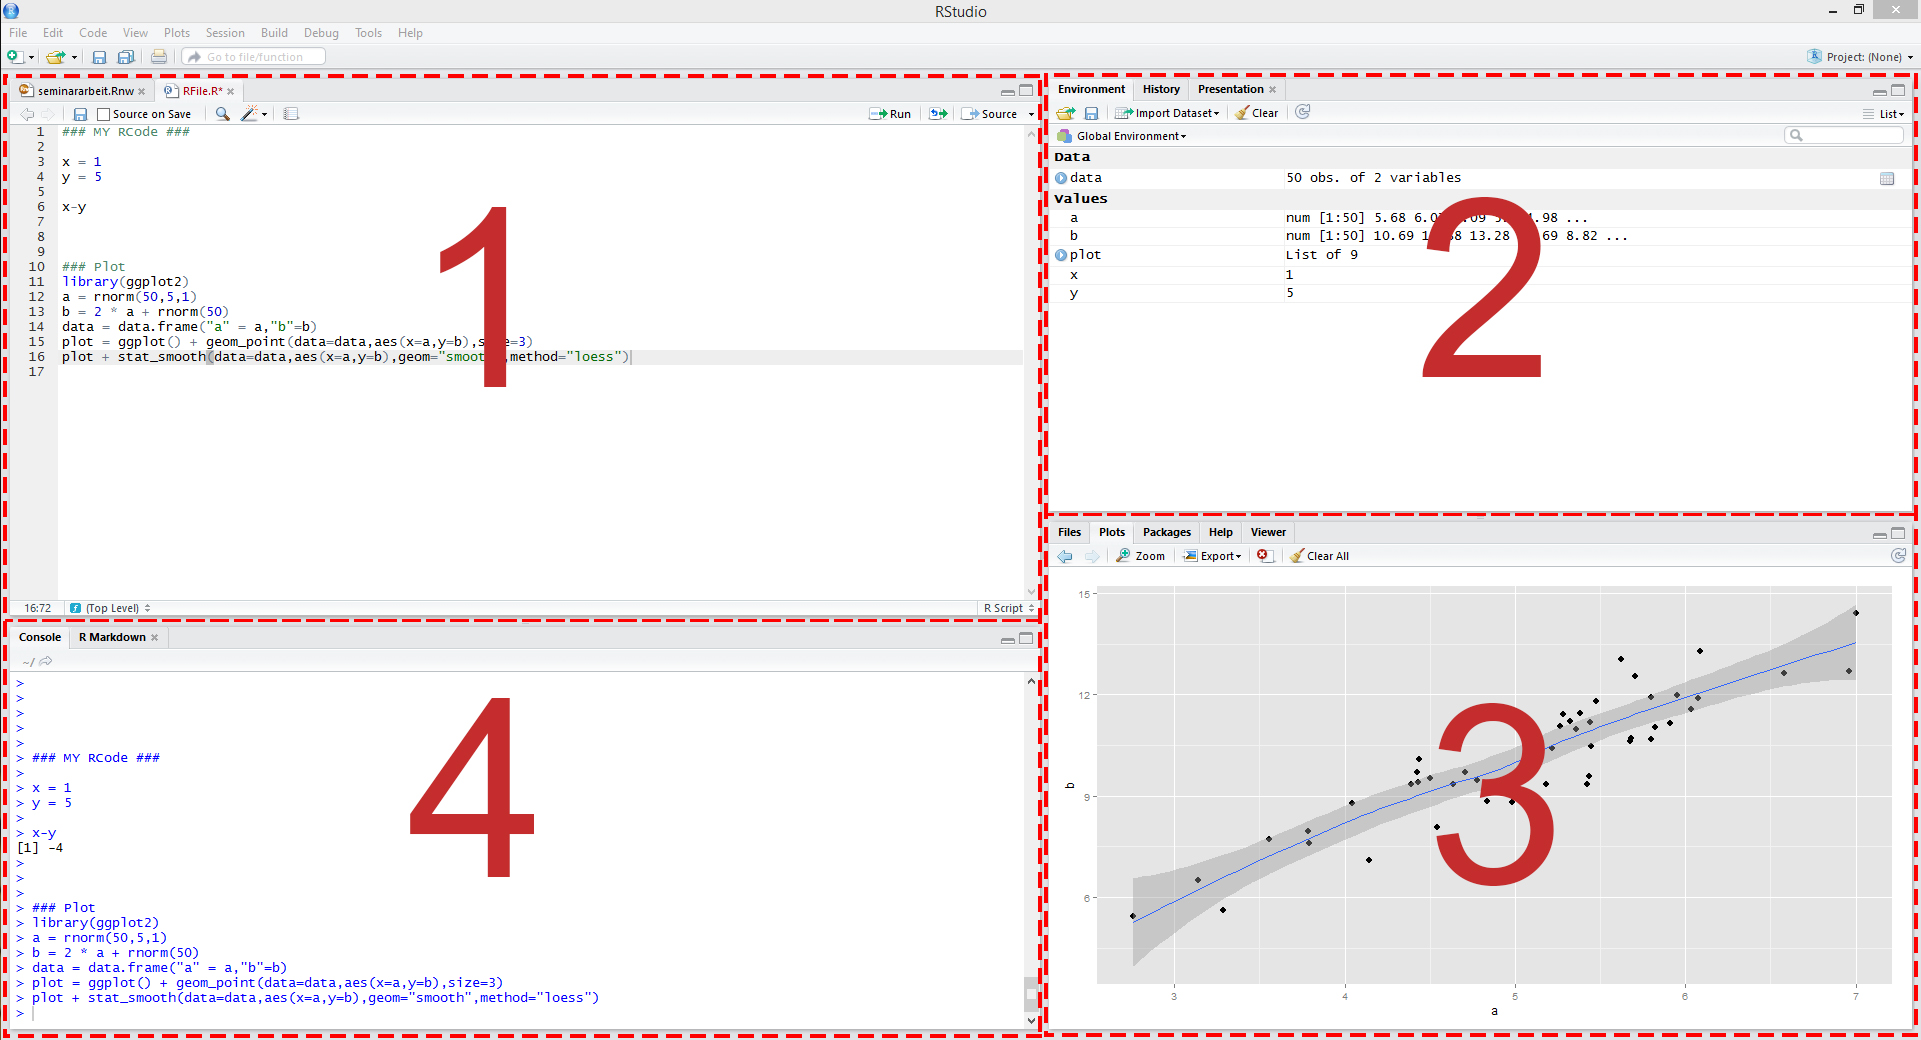
\includegraphics[width=0.8\linewidth]{images/rstudio} 

}

\caption{RStudio: empat panel}\label{fig:unnamed-chunk-4}
\end{figure}

CRAN (Comprehensive R Archive Network) adalah repositori resmi yang
menyimpan ribuan paket tambahan untuk memperluas fungsi R. Paket-paket
ini mencakup berbagai bidang aplikasi, seperti statistik, visualisasi,
dan machine learning. Untuk mengunduh dan menginstal paket di
\texttt{R}, langkah-langkahnya adalah sebagai berikut:

\begin{enumerate}
\def\labelenumi{\arabic{enumi}.}
\item
  Buka RStudio dan pastikan Anda terhubung ke internet.
\item
  Gunakan perintah install.packages() untuk menginstal library atau
  paket.
\item
  Setelah instalasi selesai, muat paket ke dalam sesi kerja
  menggunakan perintah library(). Contoh:
\end{enumerate}

\begin{Shaded}
\begin{Highlighting}[]
\FunctionTok{library}\NormalTok{(ggplot2)}
\end{Highlighting}
\end{Shaded}

Paket yang diunduh akan otomatis tersimpan di komputer Anda dan dapat
digunakan kapan saja tanpa perlu mengunduh ulang. Dengan CRAN, pengguna
dapat dengan mudah menyesuaikan \texttt{R} untuk berbagai kebutuhan
analisis data.

\subsection*{Dasar-Dasar R}\label{dasar-dasar-r}
\addcontentsline{toc}{subsection}{Dasar-Dasar R}

Seperti disebutkan sebelumnya, buku ini bukan dimaksudkan sebagai
pengantar \texttt{R}, melainkan panduan tentang cara memanfaatkan
kemampuannya untuk aplikasi yang umum analisis \emph{cluster} dengan
\texttt{R}. Pembaca yang memiliki pengetahuan dasar tentang
pemrograman \texttt{R} mungkin akan merasa nyaman untuk langsung
memulai dari \textbf{Bab} \ref{km}. Namun, bagian ini ditujukan bagi mereka
yang belum pernah bekerja dengan \texttt{R} atau \emph{RStudio}
sebelumnya. Jika Anda setidaknya sudah tahu cara membuat objek dan
memanggil fungsi, Anda bisa melewati bagian ini.

\textbf{Objek dan Variabel} Dalam \texttt{R}, \textbf{objek} adalah entitas
yang menyimpan data atau hasil perhitungan. Objek bisa berupa angka,
teks, tabel, atau bahkan fungsi. Setiap objek di \texttt{R}
memiliki nama yang digunakan untuk merujuknya dalam kode, dan objek ini
dapat disimpan ke dalam variabel untuk memudahkan manipulasi data.

\textbf{Variabel} adalah nama yang diberikan untuk menyimpan nilai atau
objek. Variabel di R tidak memerlukan deklarasi tipe data sebelumnya,
yang berarti kita dapat langsung menyimpan nilai apapun ke dalam
variabel tersebut.

Variabel dapat dibuat dengan cara memberi nama pada objek dan
menggunakan operator penugasan \texttt{\textless{}-} untuk menyimpan nilai ke dalam
variabel.

\begin{Shaded}
\begin{Highlighting}[]
\NormalTok{x }\OtherTok{\textless{}{-}} \DecValTok{5}      \CommentTok{\# Menyimpan angka 5 dalam variabel x}
\NormalTok{nama }\OtherTok{\textless{}{-}} \StringTok{"John"}  \CommentTok{\# Menyimpan string "John" dalam variabel nama}
\end{Highlighting}
\end{Shaded}

Di atas, \texttt{x} dan \texttt{nama} adalah variabel yang menyimpan objek berupa
angka dan teks.

\textbf{Mengakses Variabel} Setelah variabel dibuat, kita dapat mengakses
nilai yang tersimpan dalam variabel tersebut dengan cukup menyebutkan
nama variabel:

\begin{Shaded}
\begin{Highlighting}[]
\FunctionTok{print}\NormalTok{(x)    }\CommentTok{\# Output: 5}
\CommentTok{\#\textgreater{} [1] 5}
\end{Highlighting}
\end{Shaded}

\begin{Shaded}
\begin{Highlighting}[]
\FunctionTok{print}\NormalTok{(nama) }\CommentTok{\# Output: "John"}
\CommentTok{\#\textgreater{} [1] "John"}
\end{Highlighting}
\end{Shaded}

\subsubsection*{Tipe Data dalam Variabel}\label{tipe-data-dalam-variabel}
\addcontentsline{toc}{subsubsection}{Tipe Data dalam Variabel}

Variabel di R dapat menyimpan berbagai tipe data, antara lain:

\begin{itemize}
\item
  \textbf{Numerik:} Menyimpan angka dengan atau tanpa desimal.
\item
  \textbf{Karakter (String):} Menyimpan teks.
\item
  \textbf{Logika:} Menyimpan nilai TRUE atau FALSE.
\item
  \textbf{Faktor:} Digunakan untuk variabel kategorikal.
\item
  \textbf{Daftar (List), Vektor, Matriks, dan Data Frame}: Struktur data
  kompleks yang menyimpan koleksi data.
\end{itemize}

Contoh variabel dengan berbagai tipe data:

\begin{Shaded}
\begin{Highlighting}[]
\NormalTok{angka }\OtherTok{\textless{}{-}} \DecValTok{10}          \CommentTok{\# Numerik}
\NormalTok{nama }\OtherTok{\textless{}{-}} \StringTok{"Andi"}       \CommentTok{\# Karakter}
\NormalTok{status }\OtherTok{\textless{}{-}} \ConstantTok{TRUE}       \CommentTok{\# Logika}
\NormalTok{kategori }\OtherTok{\textless{}{-}} \FunctionTok{factor}\NormalTok{(}\FunctionTok{c}\NormalTok{(}\StringTok{"A"}\NormalTok{, }\StringTok{"B"}\NormalTok{, }\StringTok{"A"}\NormalTok{, }\StringTok{"C"}\NormalTok{))  }\CommentTok{\# Faktor}
\end{Highlighting}
\end{Shaded}

\subsubsection*{Operasi dengan Variabel}\label{operasi-dengan-variabel}
\addcontentsline{toc}{subsubsection}{Operasi dengan Variabel}

\textbf{Operasi dengan Variabel} Variabel dapat digunakan dalam operasi
matematika dan logika. Misalnya, jika kita memiliki dua variabel \texttt{a} dan
\texttt{b}, kita bisa melakukan operasi penjumlahan:

\begin{Shaded}
\begin{Highlighting}[]
\NormalTok{a }\OtherTok{\textless{}{-}} \DecValTok{3}
\NormalTok{b }\OtherTok{\textless{}{-}} \DecValTok{4}
\NormalTok{hasil }\OtherTok{\textless{}{-}}\NormalTok{ a }\SpecialCharTok{+}\NormalTok{ b  }\CommentTok{\# Menyimpan hasil penjumlahan a dan b ke dalam variabel hasil}
\FunctionTok{print}\NormalTok{(hasil)    }\CommentTok{\# Output: 7}
\CommentTok{\#\textgreater{} [1] 7}
\end{Highlighting}
\end{Shaded}

\subsubsection*{Menimpa dan Mengubah Nilai Variabel}\label{menimpa-dan-mengubah-nilai-variabel}
\addcontentsline{toc}{subsubsection}{Menimpa dan Mengubah Nilai Variabel}

\begin{Shaded}
\begin{Highlighting}[]
\NormalTok{x }\OtherTok{\textless{}{-}} \DecValTok{5}      \CommentTok{\# x sekarang bernilai 5}
\NormalTok{x }\OtherTok{\textless{}{-}} \DecValTok{10}     \CommentTok{\# x sekarang bernilai 10 (nilai sebelumnya akan tertimpa)}
\FunctionTok{print}\NormalTok{(x)    }\CommentTok{\# Output: 10}
\CommentTok{\#\textgreater{} [1] 10}
\end{Highlighting}
\end{Shaded}

\subsection*{Struktur Data pada R}\label{struktur-data-pada-r}
\addcontentsline{toc}{subsection}{Struktur Data pada R}

\texttt{R} menyediakan berbagai jenis struktur data untuk mengelola
dan memanipulasi data dalam berbagai bentuk. Pemahaman tentang struktur
data di \texttt{R} sangat penting karena memungkinkan kita untuk
menyimpan dan bekerja dengan data yang lebih kompleks. Beberapa struktur
data dasar yang tersedia di \texttt{R} meliputi vektor, matriks,
data frame, dan list.

\subsubsection*{Vektor}\label{vektor}
\addcontentsline{toc}{subsubsection}{Vektor}

Vektor adalah struktur data paling dasar di \texttt{R}. Vektor adalah sekumpulan elemen yang memiliki tipe data yang sama, seperti angka, karakter, atau logika. Vektor dapat dibuat menggunakan fungsi \texttt{c()}, yang berarti combine atau concatenate. Contoh pembuatan vektor:

\begin{Shaded}
\begin{Highlighting}[]
\NormalTok{vektor\_angka }\OtherTok{\textless{}{-}} \FunctionTok{c}\NormalTok{(}\DecValTok{1}\NormalTok{, }\DecValTok{2}\NormalTok{, }\DecValTok{3}\NormalTok{, }\DecValTok{4}\NormalTok{, }\DecValTok{5}\NormalTok{)      }\CommentTok{\# Vektor angka}
\NormalTok{vektor\_karakter }\OtherTok{\textless{}{-}} \FunctionTok{c}\NormalTok{(}\StringTok{"A"}\NormalTok{, }\StringTok{"B"}\NormalTok{, }\StringTok{"C"}\NormalTok{)   }\CommentTok{\# Vektor karakter}
\NormalTok{vektor\_logika }\OtherTok{\textless{}{-}} \FunctionTok{c}\NormalTok{(}\ConstantTok{TRUE}\NormalTok{, }\ConstantTok{FALSE}\NormalTok{, }\ConstantTok{TRUE}\NormalTok{)  }\CommentTok{\# Vektor logika}
\end{Highlighting}
\end{Shaded}

Mengakses elemen vektor:

\begin{Shaded}
\begin{Highlighting}[]
\NormalTok{vektor\_angka[}\DecValTok{1}\NormalTok{]   }\CommentTok{\# Mengakses elemen pertama (1)}
\CommentTok{\#\textgreater{} [1] 1}
\end{Highlighting}
\end{Shaded}

\begin{Shaded}
\begin{Highlighting}[]
\NormalTok{vektor\_karakter[}\DecValTok{2}\NormalTok{] }\CommentTok{\# Mengakses elemen kedua ("B")}
\CommentTok{\#\textgreater{} [1] "B"}
\end{Highlighting}
\end{Shaded}

Vektor bisa berupa vektor numerik, vektor karakter, atau vektor logika,
tergantung tipe data elemen yang ada di dalamnya.

\subsubsection*{Matriks}\label{matriks}
\addcontentsline{toc}{subsubsection}{Matriks}

Matriks adalah struktur data dua dimensi, yang berarti memiliki baris dan kolom. Semua elemen dalam matriks harus memiliki tipe data yang sama, seperti vektor. Contoh pembuatan matriks:

\begin{Shaded}
\begin{Highlighting}[]
\NormalTok{matriks }\OtherTok{\textless{}{-}} \FunctionTok{matrix}\NormalTok{(}\DecValTok{1}\SpecialCharTok{:}\DecValTok{6}\NormalTok{, }\AttributeTok{nrow =} \DecValTok{2}\NormalTok{, }\AttributeTok{ncol =} \DecValTok{3}\NormalTok{)  }\CommentTok{\# Matriks 2x3 dengan elemen dari 1 hingga 6}
\FunctionTok{print}\NormalTok{(matriks)}
\CommentTok{\#\textgreater{}      [,1] [,2] [,3]}
\CommentTok{\#\textgreater{} [1,]    1    3    5}
\CommentTok{\#\textgreater{} [2,]    2    4    6}
\end{Highlighting}
\end{Shaded}

\subsubsection*{Data Frame}\label{data-frame}
\addcontentsline{toc}{subsubsection}{Data Frame}

Data frame adalah struktur data yang lebih kompleks dan sering digunakan dalam analisis data. Data frame terdiri dari kolom-kolom yang dapat memiliki tipe data yang berbeda (numerik, karakter, logika, dll.), mirip dengan tabel dalam basis data atau spreadsheet. Contoh pembuatan data frame:

\begin{Shaded}
\begin{Highlighting}[]
\NormalTok{df }\OtherTok{\textless{}{-}} \FunctionTok{data.frame}\NormalTok{(}
  \AttributeTok{Nama =} \FunctionTok{c}\NormalTok{(}\StringTok{"John"}\NormalTok{, }\StringTok{"Alice"}\NormalTok{, }\StringTok{"Bob"}\NormalTok{),}
  \AttributeTok{Umur =} \FunctionTok{c}\NormalTok{(}\DecValTok{25}\NormalTok{, }\DecValTok{30}\NormalTok{, }\DecValTok{22}\NormalTok{),}
  \AttributeTok{Status =} \FunctionTok{c}\NormalTok{(}\StringTok{"Single"}\NormalTok{, }\StringTok{"Married"}\NormalTok{, }\StringTok{"Single"}\NormalTok{)}
\NormalTok{)}
\FunctionTok{print}\NormalTok{(df)}
\CommentTok{\#\textgreater{}    Nama Umur  Status}
\CommentTok{\#\textgreater{} 1  John   25  Single}
\CommentTok{\#\textgreater{} 2 Alice   30 Married}
\CommentTok{\#\textgreater{} 3   Bob   22  Single}
\end{Highlighting}
\end{Shaded}

\subsubsection*{List}\label{list}
\addcontentsline{toc}{subsubsection}{List}

List adalah struktur data yang paling fleksibel di \texttt{R}. List dapat menyimpan berbagai jenis objek yang berbeda dalam satu struktur data, termasuk vektor, matriks, data frame, atau bahkan fungsi. Contoh pembuatan list:

\begin{Shaded}
\begin{Highlighting}[]
\NormalTok{daftar }\OtherTok{\textless{}{-}} \FunctionTok{list}\NormalTok{(}
  \AttributeTok{Nama =} \StringTok{"John"}\NormalTok{,}
  \AttributeTok{Umur =} \DecValTok{25}\NormalTok{,}
  \AttributeTok{Nilai =} \FunctionTok{c}\NormalTok{(}\DecValTok{90}\NormalTok{, }\DecValTok{85}\NormalTok{, }\DecValTok{88}\NormalTok{)}
\NormalTok{)}
\FunctionTok{print}\NormalTok{(daftar)}
\CommentTok{\#\textgreater{} $Nama}
\CommentTok{\#\textgreater{} [1] "John"}
\CommentTok{\#\textgreater{} }
\CommentTok{\#\textgreater{} $Umur}
\CommentTok{\#\textgreater{} [1] 25}
\CommentTok{\#\textgreater{} }
\CommentTok{\#\textgreater{} $Nilai}
\CommentTok{\#\textgreater{} [1] 90 85 88}
\end{Highlighting}
\end{Shaded}

\subsubsection*{Vektor}\label{vektor-1}
\addcontentsline{toc}{subsubsection}{Vektor}

Faktor adalah tipe data di \texttt{R} yang digunakan untuk menyimpan data kategorikal. Faktor menyimpan data dalam bentuk level yang dapat digunakan untuk analisis kategorikal, seperti dalam model regresi atau analisis statistik lainnya. Contoh pembuatan faktor:

\begin{Shaded}
\begin{Highlighting}[]
\NormalTok{status }\OtherTok{\textless{}{-}} \FunctionTok{factor}\NormalTok{(}\FunctionTok{c}\NormalTok{(}\StringTok{"Single"}\NormalTok{, }\StringTok{"Married"}\NormalTok{, }\StringTok{"Single"}\NormalTok{, }\StringTok{"Divorced"}\NormalTok{))}
\FunctionTok{print}\NormalTok{(status)}
\CommentTok{\#\textgreater{} [1] Single   Married  Single   Divorced}
\CommentTok{\#\textgreater{} Levels: Divorced Married Single}
\end{Highlighting}
\end{Shaded}

\textbf{Berikut adalah perbandingan antara berbagai struktur data di R:}

\begin{longtable}[]{@{}
  >{\raggedright\arraybackslash}p{(\columnwidth - 4\tabcolsep) * \real{0.3333}}
  >{\raggedright\arraybackslash}p{(\columnwidth - 4\tabcolsep) * \real{0.3333}}
  >{\raggedright\arraybackslash}p{(\columnwidth - 4\tabcolsep) * \real{0.3333}}@{}}
\toprule\noalign{}
\begin{minipage}[b]{\linewidth}\raggedright
Struktur Data
\end{minipage} & \begin{minipage}[b]{\linewidth}\raggedright
Deskripsi
\end{minipage} & \begin{minipage}[b]{\linewidth}\raggedright
Contoh Penggunaan
\end{minipage} \\
\midrule\noalign{}
\endhead
\bottomrule\noalign{}
\endlastfoot
Vektor & Sekumpulan elemen dengan tipe data yang sama & Menyimpan data numerik atau karakter \\
Matriks & Struktur dua dimensi (baris dan kolom) & Menyimpan data dalam bentuk tabel numerik \\
Data Frame & Tabel dua dimensi dengan tipe data berbeda & Menyimpan data observasi dan variabel \\
List & Koleksi elemen dengan tipe data yang berbeda & Menyimpan objek dengan tipe data campuran \\
Faktor & Data kategorikal dengan level yang terbatas & Mengelompokkan data kategorikal \\
\end{longtable}

\subsection*{Fungsi dan Pemrograman di R}\label{fungsi-dan-pemrograman-di-r}
\addcontentsline{toc}{subsection}{Fungsi dan Pemrograman di R}

\texttt{R} menyediakan berbagai cara untuk mendefinisikan dan menggunakan fungsi dalam pemrograman. Fungsi adalah blok kode yang dirancang untuk melakukan tugas tertentu, menerima input, dan memberikan output. Pemrograman berbasis fungsi memungkinkan pengguna untuk menulis kode yang lebih modular dan terstruktur, yang memudahkan pemeliharaan dan pengembangan program.

\subsubsection*{Definisi Fungsi}\label{definisi-fungsi}
\addcontentsline{toc}{subsubsection}{Definisi Fungsi}

Fungsi di \texttt{R} dibuat menggunakan kata kunci \texttt{function()}. Fungsi ini dapat menerima satu atau lebih argumen dan menghasilkan nilai output. Contoh pembuatan fungsi:

\begin{Shaded}
\begin{Highlighting}[]
\CommentTok{\# Fungsi untuk menghitung kuadrat suatu angka}
\NormalTok{kuadrat }\OtherTok{\textless{}{-}} \ControlFlowTok{function}\NormalTok{(x) \{}
  \FunctionTok{return}\NormalTok{(x}\SpecialCharTok{\^{}}\DecValTok{2}\NormalTok{)   }\CommentTok{\# Mengembalikan nilai kuadrat dari x}
\NormalTok{\}}
\end{Highlighting}
\end{Shaded}

\subsubsection*{Pemanggilan fungsi}\label{pemanggilan-fungsi}
\addcontentsline{toc}{subsubsection}{Pemanggilan fungsi}

\begin{Shaded}
\begin{Highlighting}[]
\NormalTok{hasil }\OtherTok{\textless{}{-}} \FunctionTok{kuadrat}\NormalTok{(}\DecValTok{5}\NormalTok{)  }\CommentTok{\# Memanggil fungsi \textquotesingle{}kuadrat\textquotesingle{} dengan argumen 5}
\FunctionTok{print}\NormalTok{(hasil)          }\CommentTok{\# Output: 25}
\CommentTok{\#\textgreater{} [1] 25}
\end{Highlighting}
\end{Shaded}

\subsubsection*{Argumen fungsi}\label{argumen-fungsi}
\addcontentsline{toc}{subsubsection}{Argumen fungsi}

Fungsi di \texttt{R} dapat menerima berbagai jenis argumen, yang bisa berupa variabel, nilai tetap, atau objek lain. Argumen juga bisa diberikan nilai default, yang berarti fungsi tetap dapat dipanggil meskipun beberapa argumen tidak diberikan nilai. Contoh argumen dengan nilai default:

\begin{Shaded}
\begin{Highlighting}[]
\CommentTok{\# Fungsi untuk menghitung hasil pembagian}
\NormalTok{bagi }\OtherTok{\textless{}{-}} \ControlFlowTok{function}\NormalTok{(a, }\AttributeTok{b =} \DecValTok{2}\NormalTok{) \{}
  \FunctionTok{return}\NormalTok{(a }\SpecialCharTok{/}\NormalTok{ b)  }\CommentTok{\# Jika b tidak diberikan, akan menggunakan nilai default 2}
\NormalTok{\}}

\FunctionTok{print}\NormalTok{(}\FunctionTok{bagi}\NormalTok{(}\DecValTok{10}\NormalTok{))   }\CommentTok{\# Output: 5 (10 dibagi 2)}
\CommentTok{\#\textgreater{} [1] 5}
\end{Highlighting}
\end{Shaded}

\begin{Shaded}
\begin{Highlighting}[]
\FunctionTok{print}\NormalTok{(}\FunctionTok{bagi}\NormalTok{(}\DecValTok{10}\NormalTok{, }\DecValTok{5}\NormalTok{)) }\CommentTok{\# Output: 2 (10 dibagi 5)}
\CommentTok{\#\textgreater{} [1] 2}
\end{Highlighting}
\end{Shaded}

\subsubsection*{Fungsi dengan Beberapa Nilai Kembalian}\label{fungsi-dengan-beberapa-nilai-kembalian}
\addcontentsline{toc}{subsubsection}{Fungsi dengan Beberapa Nilai Kembalian}

Fungsi di \texttt{R} dapat mengembalikan lebih dari satu nilai. Salah satu cara untuk melakukan ini adalah dengan menggunakan list. Fungsi dapat mengembalikan objek yang lebih kompleks, seperti list, untuk menyimpan beberapa hasil sekaligus. Contoh fungsi dengan beberapa nilai kembalian:

\begin{Shaded}
\begin{Highlighting}[]
\NormalTok{hasil\_operasi }\OtherTok{\textless{}{-}} \ControlFlowTok{function}\NormalTok{(a, b) \{}
\NormalTok{  hasil\_penjumlahan }\OtherTok{\textless{}{-}}\NormalTok{ a }\SpecialCharTok{+}\NormalTok{ b}
\NormalTok{  hasil\_perkalian }\OtherTok{\textless{}{-}}\NormalTok{ a }\SpecialCharTok{*}\NormalTok{ b}
  \FunctionTok{return}\NormalTok{(}\FunctionTok{list}\NormalTok{(}\AttributeTok{penjumlahan =}\NormalTok{ hasil\_penjumlahan, }\AttributeTok{perkalian =}\NormalTok{ hasil\_perkalian))}
\NormalTok{\}}

\NormalTok{output }\OtherTok{\textless{}{-}} \FunctionTok{hasil\_operasi}\NormalTok{(}\DecValTok{4}\NormalTok{, }\DecValTok{5}\NormalTok{)}
\FunctionTok{print}\NormalTok{(output}\SpecialCharTok{$}\NormalTok{penjumlahan)  }\CommentTok{\# Output: 9}
\CommentTok{\#\textgreater{} [1] 9}
\end{Highlighting}
\end{Shaded}

\begin{Shaded}
\begin{Highlighting}[]
\FunctionTok{print}\NormalTok{(output}\SpecialCharTok{$}\NormalTok{perkalian)    }\CommentTok{\# Output: 20}
\CommentTok{\#\textgreater{} [1] 20}
\end{Highlighting}
\end{Shaded}

\subsubsection*{Fungsi Bawaan di R}\label{fungsi-bawaan-di-r}
\addcontentsline{toc}{subsubsection}{Fungsi Bawaan di R}

\texttt{R} menyediakan banyak fungsi bawaan untuk melakukan berbagai tugas, seperti manipulasi data, analisis statistik, dan visualisasi. Fungsi-fungsi ini sangat berguna dan sering digunakan dalam berbagai analisis. Contoh fungsi bawaan:

\begin{Shaded}
\begin{Highlighting}[]
\CommentTok{\# Fungsi untuk menghitung rata{-}rata}
\NormalTok{rata\_rata }\OtherTok{\textless{}{-}} \FunctionTok{mean}\NormalTok{(}\FunctionTok{c}\NormalTok{(}\DecValTok{1}\NormalTok{, }\DecValTok{2}\NormalTok{, }\DecValTok{3}\NormalTok{, }\DecValTok{4}\NormalTok{, }\DecValTok{5}\NormalTok{))  }\CommentTok{\# Output: 3}
\FunctionTok{print}\NormalTok{(rata\_rata)}
\CommentTok{\#\textgreater{} [1] 3}
\end{Highlighting}
\end{Shaded}

\subsubsection*{Fungsi Anonim}\label{fungsi-anonim}
\addcontentsline{toc}{subsubsection}{Fungsi Anonim}

Fungsi anonim adalah fungsi yang tidak memiliki nama. Fungsi jenis ini sering digunakan dalam operasi sementara atau dalam konteks tertentu, seperti dalam operasi dengan apply atau pemrograman berbasis vektor. Contoh fungsi anonim:

\begin{Shaded}
\begin{Highlighting}[]
\CommentTok{\# Menggunakan fungsi anonim dalam apply}
\NormalTok{angka }\OtherTok{\textless{}{-}} \FunctionTok{c}\NormalTok{(}\DecValTok{1}\NormalTok{, }\DecValTok{2}\NormalTok{, }\DecValTok{3}\NormalTok{, }\DecValTok{4}\NormalTok{, }\DecValTok{5}\NormalTok{)}
\NormalTok{hasil }\OtherTok{\textless{}{-}} \FunctionTok{sapply}\NormalTok{(angka, }\ControlFlowTok{function}\NormalTok{(x) x}\SpecialCharTok{\^{}}\DecValTok{2}\NormalTok{)  }\CommentTok{\# Menerapkan fungsi untuk menghitung kuadrat}
\FunctionTok{print}\NormalTok{(hasil)  }\CommentTok{\# Output: 1 4 9 16 25}
\CommentTok{\#\textgreater{} [1]  1  4  9 16 25}
\end{Highlighting}
\end{Shaded}

Semua perintah yang telah dijelaskan di atas juga dapat
digunakan pada widget interaktif di seluruh buku ini. Anda dapat
mencobanya di bawah ini.

\begin{center}
\textit{This interactive application is only available in the HTML version.}
\end{center}

\part{Pendekatan Partisi}\label{part-pendekatan-partisi}

\chapter{Algoritma K-Means}\label{km}

\begin{quote}
``It's not the data that's important, it's the story the data tells''

-- Moneyball
\end{quote}

Algoritma K-Means merupakan salah satu metode yang paling populer dalam analisis \emph{cluster}, yang digunakan untuk mengelompokkan data ke dalam beberapa kelompok berdasarkan kesamaan fitur \citep{jain2010} . Metode ini bekerja dengan cara membagi data ke dalam \(K\) cluster, di mana \(K\) adalah jumlah \emph{cluster} yang ditentukan sebelumnya oleh pengguna \citep{macqueen1967some}. Proses pengelompokan ini dilakukan dengan meminimalkan jarak antara data dalam satu \emph{cluster} dan pusat \emph{cluster} (centroid) yang dihasilkan. Langkah pertama dalam algoritma K-Means adalah inisialisasi centroid untuk setiap \emph{cluster}, yang dapat dilakukan secara acak atau menggunakan metode tertentu seperti K-Means++ \citep{arthur2007kmeans}. Setelah centroid diinisialisasi, algoritma kemudian mengelompokkan setiap data ke dalam \emph{cluster} terdekat berdasarkan jarak Euclidean\citep{hastie2009elements}. Proses ini diulang hingga tidak ada perubahan signifikan dalam posisi \emph{centroid} atau tidak ada perubahan dalam pengelompokan data.

Salah satu keunggulan dari algoritma K-Means adalah kesederhanaannya, yang membuatnya mudah dipahami dan diimplementasikan, bahkan oleh pemula \citep{han2011data}. Namun, algoritma ini juga memiliki beberapa kelemahan, seperti ketergantungan pada pemilihan jumlah \emph{cluster} \(K\) yang tepat dan sensitivitas terhadap \emph{outlier}. Oleh karena itu, pemilihan \(K\) yang optimal sering kali menjadi tantangan tersendiri dalam penerapan algoritma ini \citep{elbow1975outline}. Dalam praktiknya, algorima K-Means banyak digunakan dalam berbagai bidang, termasuk pemasaran, pengenalan pola, dan analisis citra \citep{xu2005survey}. Misalnya, dalam pemasaran, K-Means dapat digunakan untuk segmentasi pelanggan berdasarkan perilaku pembelian mereka, sehingga perusahaan dapat menargetkan strategi pemasaran yang lebih efektif \citep{kumar2016creating}. Dengan demikian, pemahaman yang baik tentang algoritma K-Means sangat penting bagi para peneliti dan praktisi yang ingin menerapkan analisis \emph{cluster} dalam pekerjaan mereka.

Secara keseluruhan, algoritma K-Means adalah alat yang kuat dan fleksibel untuk analisis \emph{cluster}, meskipun penggunaannya memerlukan pemahaman yang mendalam tentang data dan konteks analisis \citep{bishop2006pattern}. Dalam buku ini, kami akan membahas secara rinci tentang cara menerapkan algoritma K-Means menggunakan \texttt{R}, serta memberikan panduan langkah demi langkah untuk membantu pemula memahami dan menguasai teknik ini. Dengan demikian, diharapkan pembaca dapat memanfaatkan algoritma K-Means dalam analisis data mereka secara efektif.

\section{Tahapan Algoritma K-Means}\label{tahapan-algoritma-k-means}

\subsection*{1. Inisialisasi Centroid}\label{inisialisasi-centroid}
\addcontentsline{toc}{subsection}{1. Inisialisasi Centroid}

Pilih jumlah cluster \(k\) yang diinginkan. Inisialisasi \(k\) centroid secara acak dari dataset. Centroid adalah titik yang mewakili pusat dari setiap cluster.

\[
C_k = (x_{k1}, x_{k2}, \ldots, x_{kn}) \quad \text{untuk } k = 1, 2, \ldots, K
\]
di mana \(C_k\) adalah centroid untuk cluster ke-\(k\) dan \(x_{ki}\) adalah nilai fitur ke-\(i\) dari centroid ke-\(k\).

\subsection*{2. Penugasan Cluster}\label{penugasan-cluster}
\addcontentsline{toc}{subsection}{2. Penugasan Cluster}

Untuk setiap titik data \(x_i\), hitung jarak ke setiap centroid \(C_k\) dan tetapkan titik data tersebut ke cluster dengan centroid terdekat. Jarak yang umum digunakan adalah jarak Euclidean.

\[
d(x_i, C_k) = \sqrt{\sum_{j=1}^{m} (x_{ij} - C_{kj})^2}
\]
di mana \(d(x_i, C_k)\) adalah jarak antara titik data \(x_i\) dan centroid \(C_k\), \(m\) adalah jumlah fitur, dan \(x_{ij}\) adalah nilai fitur ke-\(j\) dari titik data ke-\(i\).

Penugasan cluster dapat dinyatakan sebagai:

\[
\text{Cluster}(x_i) = \arg\min_{k} d(x_i, C_k)
\]

\subsection*{3. Perbaharui Centroid}\label{perbaharui-centroid}
\addcontentsline{toc}{subsection}{3. Perbaharui Centroid}

Setelah semua titik data ditugaskan ke cluster, hitung ulang posisi centroid untuk setiap cluster dengan mengambil rata-rata dari semua titik data yang ditugaskan ke cluster tersebut.

\[
C_k = \frac{1}{N_k} \sum_{x_i \in \text{Cluster}_k} x_i
\]
di mana \(N_k\) adalah jumlah titik data dalam cluster ke-\(k\) dan \(\text{Cluster}_k\) adalah himpunan titik data yang ditugaskan ke cluster ke-\(k\).

\subsection*{4. Ulangi Langkah 2 dan 3}\label{ulangi-langkah-2-dan-3}
\addcontentsline{toc}{subsection}{4. Ulangi Langkah 2 dan 3}

Ulangi langkah penugasan cluster dan pembaruan centroid hingga tidak ada perubahan signifikan dalam posisi centroid atau tidak ada perubahan dalam pengelompokan data. Kriteria konvergensi dapat berupa:

\[
\text{Jika } \| C_k^{(t)} - C_k^{(t-1)} \| < \epsilon \quad \text{atau tidak ada perubahan cluster}
\]

di mana \(\epsilon\) adalah ambang batas kecil yang ditentukan sebelumnya.

\subsection*{5. Hasil Akhir}\label{hasil-akhir}
\addcontentsline{toc}{subsection}{5. Hasil Akhir}

Setelah konvergensi tercapai, hasil akhir adalah centroid dari setiap cluster dan pengelompokan titik data ke dalam cluster yang sesuai.

\section{Eksperimen Algoritma K-Means}\label{eksperimen-algoritma-k-means}

\subsection*{Deskripsi Data}\label{deskripsi-data}
\addcontentsline{toc}{subsection}{Deskripsi Data}

Data yang digunakan dalam eksperimen k-means ini berasal dari Tim Percepatan Penanggulangan Kemiskinan \href{https://www.tnp2k.go.id/}{(TNP2K)}. TNP2K merupakan lembaga yang bertugas untuk merumuskan dan melaksanakan kebijakan serta program penanggulangan kemiskinan di Indonesia. Data yang diperoleh mencakup berbagai variabel yang relevan untuk analisis kemiskinan, termasuk indikator sosial, ekonomi, dan demografis. Penggunaan data ini bertujuan untuk mengidentifikasi pola dan kelompok dalam populasi yang berpotensi mengalami kemiskinan, sehingga dapat membantu dalam merumuskan strategi yang lebih efektif dalam penanggulangan kemiskinan. Melalui metode k-means, kami berharap dapat menemukan segmentasi yang jelas dalam data, yang pada gilirannya dapat memberikan wawasan yang lebih mendalam mengenai karakteristik kelompok-kelompok yang rentan terhadap kemiskinan.

\subsection*{Data}\label{data}
\addcontentsline{toc}{subsection}{Data}

Dengan menggunakan fungsi \texttt{read.csv()} dari \texttt{R}, kami dapat mengimpor data langsung dari URL tersebut ke dalam lingkungan kerja \texttt{R}. Berikut adalah kode yang digunakan untuk membaca data:
Package \texttt{reader} menyiapkan fungsi \href{https://readr.tidyverse.org/reference/read_delim.html}{\texttt{read\_csv()}} untuk import data dari file CSV. Pada kasus ini digunakan data \href{https://github.com/dedenistiawan/Dataset/blob/main/BDT.csv}{Data 40\% Kemiskinan di jawa Tengah}.

\begin{Shaded}
\begin{Highlighting}[]
\FunctionTok{library}\NormalTok{ (readr)}
\NormalTok{urlfile }\OtherTok{=} \StringTok{"https://bit.ly/3VO3kRE"}
\NormalTok{data}\OtherTok{\textless{}{-}}\FunctionTok{read.csv}\NormalTok{(}\FunctionTok{url}\NormalTok{(urlfile), }\AttributeTok{row.names =} \StringTok{"Kabupaten"}\NormalTok{)}
\end{Highlighting}
\end{Shaded}

\begin{table}

\caption{\label{tab:nice-tab-km}Basis Data Terpadu Jawa Tengah}
\centering
\begin{tabular}[t]{lrrrrrrrrrr}
\toprule
  & X1 & X2 & X3 & X4 & X5 & X6 & X7 & X8 & X9 & X10\\
\midrule
CILACAP & 5.19 & 5.67 & 5.08 & 5.44 & 5.22 & 6.05 & 11.47 & 9.78 & 5.55 & 5.12\\
BANYUMAS & 5.71 & 4.47 & 5.18 & 5.51 & 5.02 & 6.21 & 7.39 & 6.96 & 5.98 & 8.22\\
PURBALINGGA & 3.30 & 2.19 & 3.80 & 3.13 & 3.73 & 3.34 & 8.71 & 7.41 & 3.21 & 4.65\\
BANJARNEGARA & 2.73 & 2.34 & 3.76 & 2.80 & 2.57 & 2.99 & 3.31 & 5.45 & 4.21 & 6.05\\
KEBUMEN & 4.17 & 2.55 & 3.26 & 4.16 & 3.15 & 4.15 & 4.30 & 9.29 & 4.61 & 4.34\\
\addlinespace
PURWOREJO & 1.87 & 2.12 & 1.48 & 3.05 & 1.78 & 1.83 & 5.00 & 4.90 & 3.12 & 2.09\\
WONOSOBO & 2.13 & 1.95 & 3.00 & 1.78 & 1.62 & 2.06 & 0.45 & 2.32 & 3.57 & 0.84\\
MAGELANG & 3.95 & 3.01 & 4.22 & 4.15 & 3.01 & 3.64 & 1.44 & 3.35 & 5.69 & 3.67\\
BOYOLALI & 2.19 & 3.07 & 1.61 & 2.74 & 2.11 & 1.82 & 1.71 & 2.34 & 3.41 & 1.55\\
KLATEN & 3.84 & 5.15 & 1.93 & 4.64 & 4.04 & 3.78 & 8.71 & 4.45 & 3.99 & 3.09\\
\bottomrule
\end{tabular}
\end{table}

\subsection*{\texorpdfstring{Memeriksa \emph{Missing Value}}{Memeriksa Missing Value}}\label{memeriksa-missing-value}
\addcontentsline{toc}{subsection}{Memeriksa \emph{Missing Value}}

Sebelum melakukan analisis cluster menggunakan metode k-means, penting untuk memeriksa apakah terdapat nilai yang hilang (missing values) dalam dataset. Nilai yang hilang dapat mempengaruhi hasil analisis dan interpretasi data, sehingga perlu ditangani dengan tepat. Kami akan menggunakan fungsi \texttt{is.na()} dan \texttt{colsum()} untuk menghitung jumlah nilai yang hilang dalam setiap kolom dari dataset. Jika ditemukan nilai yang hilang, langkah selanjutnya adalah memutuskan bagaimana cara menanganinya, apakah dengan menghapus baris yang mengandung nilai hilang, mengganti nilai hilang dengan rata-rata, median, atau metode imputasi lainnya.

Berikut adalah kode untuk memeriksa nilai yang hilang dalam dataset:

\begin{Shaded}
\begin{Highlighting}[]
\FunctionTok{colSums}\NormalTok{(}\FunctionTok{is.na}\NormalTok{(data))}
\CommentTok{\#\textgreater{}  X1  X2  X3  X4  X5  X6  X7  X8  X9 X10 }
\CommentTok{\#\textgreater{}   0   0   0   0   0   0   0   0   0   0}
\end{Highlighting}
\end{Shaded}

Setelah melakukan pemeriksaan terhadap dataset, tidak ada nilai yang hilang (\emph{missing values}) dalam data yang kami gunakan. Hal ini penting karena keberadaan nilai yang hilang dapat mempengaruhi hasil analisis dan interpretasi data.

\subsection*{Visualisasi Matriks jarak}\label{visualisasi-matriks-jarak}
\addcontentsline{toc}{subsection}{Visualisasi Matriks jarak}

Setelah mempersiapkan data dan memastikan tidak ada nilai yang hilang, langkah selanjutnya adalah membuat visualisasi matriks jarak. Visualisasi ini penting untuk memahami seberapa dekat atau jauh objek-objek dalam dataset berdasarkan variabel yang ada. Dengan menggunakan matriks jarak, kita dapat melihat pola dan hubungan antar data yang akan membantu dalam analisis \emph{cluster}. Kami akan menggunakan library \texttt{factoextra} untuk menghitung dan memvisualisasikan matriks jarak. Fungsi \texttt{get\_dist()} akan digunakan untuk menghitung jarak antar objek, dan \texttt{fviz\_dist()} dari \texttt{factoextra} akan digunakan untuk membuat visualisasi. Berikut adalah kode untuk membuat visualisasi matriks jarak:

\begin{Shaded}
\begin{Highlighting}[]
\FunctionTok{library}\NormalTok{(ggplot2)}
\FunctionTok{library}\NormalTok{(factoextra)}
\NormalTok{distance }\OtherTok{\textless{}{-}} \FunctionTok{get\_dist}\NormalTok{(data)}
\FunctionTok{fviz\_dist}\NormalTok{(distance, }\AttributeTok{gradient =} \FunctionTok{list}\NormalTok{(}\AttributeTok{low =} \StringTok{"\#00AFBB"}\NormalTok{, }\AttributeTok{mid =} \StringTok{"white"}\NormalTok{, }\AttributeTok{high =} \StringTok{"\#FC4E07"}\NormalTok{))}
\end{Highlighting}
\end{Shaded}

\begin{figure}[h]

{\centering \includegraphics[width=0.8\linewidth]{02-ch2_files/figure-latex/unnamed-chunk-4-1} 

}

\caption{Matrik Jarak}\label{fig:unnamed-chunk-4}
\end{figure}

Setelah membuat visualisasi matriks jarak, kita dapat melakukan analisis untuk memahami pola dan hubungan antar objek dalam dataset. Matriks jarak memberikan informasi tentang seberapa mirip atau berbeda objek-objek dalam data berdasarkan variabel yang digunakan.

Dalam visualisasi matriks jarak yang telah dibuat, kita dapat mengamati beberapa hal:

\begin{enumerate}
\def\labelenumi{\arabic{enumi}.}
\item
  \textbf{Warna dan Jarak}:
  Warna yang lebih gelap menunjukkan jarak yang lebih dekat antara objek, sedangkan warna yang lebih terang menunjukkan jarak yang lebih jauh. Dengan demikian, objek-objek yang memiliki warna serupa cenderung memiliki karakteristik yang lebih mirip.
\item
  \textbf{Kelompok Objek}:
  Dari visualisasi, kita dapat mengidentifikasi kelompok objek yang mungkin memiliki kesamaan. Misalnya, jika terdapat beberapa objek yang berdekatan dan memiliki warna yang sama, ini menunjukkan bahwa mereka mungkin termasuk dalam cluster yang sama.
\item
  \textbf{Outlier}:
  Objek yang jauh dari kelompok lainnya dapat dianggap sebagai outlier. Outlier ini mungkin memiliki karakteristik yang unik atau berbeda dari mayoritas data, dan perlu dianalisis lebih lanjut untuk memahami penyebab perbedaannya.
\end{enumerate}

Selanjutnya, kita dapat melanjutkan dengan analisis cluster menggunakan algoritma k-means untuk mengelompokkan objek-objek dalam dataset berdasarkan jarak yang telah dihitung. Dengan demikian, kita dapat lebih memahami pola dalam data dan membuat keputusan yang lebih baik berdasarkan hasil analisis.

\subsection*{\texorpdfstring{Estimasi Jumlah \emph{Cluster} Optimal}{Estimasi Jumlah Cluster Optimal}}\label{estimasi-jumlah-cluster-optimal}
\addcontentsline{toc}{subsection}{Estimasi Jumlah \emph{Cluster} Optimal}

Dalam metode k-means banyaknya klaster ditentukan sendiri oleh pengguna. Maka dari itu perlu dicari jumlah klaster yang optimum yang dapat mengelompokkan objek dengan baik (Perlu diketahui bahwa metode ini relatif subjektif). Salah satu metode yang digunakan adalah Elbow Plot. Elbow Plot merupakan plot antara banyak klaster dengan total within-cluster variation (total dari simpangan per kluster). Banyak klaster yang dipilih adalah bagian ``siku'' atau titik dimana terdapat penurunan yang tajam sebelum titik tersebut dan disusul penurunan yang tidak tajam setelah titik tersebut. Hal ini karena penambahan jumlah klaster tidak membawa pengaruh banyak atas variasi yang ada di dalam klaster tersebut.

\subsection*{Metode Elbow}\label{metode-elbow}
\addcontentsline{toc}{subsection}{Metode Elbow}

Metode Elbow merupakan suatu metode yang digunakan untuk menghasilkan informasi dalam menentukan jumlah cluster terbaik dengan cara melihat persentase hasil perbandingan antara jumlah cluster yang akan membentuk siku pada suatu titik. Metode ini memberikan ide/gagasan dengan cara memilih nilai cluster dan kemudian menambah nilai cluster tersebut untuk dijadikan model data dalam penentuan cluster terbaik. Dan selain itu persentase perhitungan yang dihasilkan menjadi pembanding antara jumlah cluster yang ditambah. Hasil persentase yang berbeda dari setiap nilai cluster dapat ditunjukan dengan menggunakan grafik sebagai sumber informasinya. Jika nilai cluster pertama dengan nilai cluster kedua memberikan sudut dalam grafik atau nilainya mengalami penurunan paling besar maka nilai cluster tersebut yang terbaik.

\begin{Shaded}
\begin{Highlighting}[]
\CommentTok{\#penentuan jumlah cluster optimal}
\FunctionTok{library}\NormalTok{(ggplot2)}
\FunctionTok{library}\NormalTok{(factoextra)}
\FunctionTok{fviz\_nbclust}\NormalTok{(data, kmeans, }\AttributeTok{method =} \StringTok{"wss"}\NormalTok{) }\SpecialCharTok{+}
  \FunctionTok{geom\_vline}\NormalTok{(}\AttributeTok{xintercept =} \DecValTok{2}\NormalTok{, }\AttributeTok{linetype =} \DecValTok{2}\NormalTok{)}
\end{Highlighting}
\end{Shaded}

\begin{figure}[h]

{\centering \includegraphics[width=0.8\linewidth]{02-ch2_files/figure-latex/unnamed-chunk-5-1} 

}

\caption{Plot Jumlah Cluster Metode Elbow}\label{fig:unnamed-chunk-5}
\end{figure}

Metode elbow menggunakan nilai total wss (whitin sum square) sebagai penentu \(k\) optimalnya. Dari gambar di atas terlihat garis mengalami patahan yang membentuk elbow atau siku pada saat \(k=2\). Maka dengan menggunakan metode ini diperoleh \(k\) optimal pada saat berada di \(k=2\).

\subsection*{Metode Silhouette}\label{metode-silhouette}
\addcontentsline{toc}{subsection}{Metode Silhouette}

Silhouette Coefficient digunakan untuk melihat kualitas dan kekuatan cluster, seberapa baik suatu objek ditempatkan dalam suatu cluster. Metode ini merupakan gabungan dari metode cohesion dan separation.

\begin{Shaded}
\begin{Highlighting}[]
\DocumentationTok{\#\#Average Silhouette Method}
\FunctionTok{fviz\_nbclust}\NormalTok{(data, kmeans, }\AttributeTok{method =} \StringTok{"silhouette"}\NormalTok{)}
\end{Highlighting}
\end{Shaded}

\begin{figure}[h]

{\centering \includegraphics[width=0.8\linewidth]{02-ch2_files/figure-latex/unnamed-chunk-6-1} 

}

\caption{Plot Jumlah Cluster Metode silhouette}\label{fig:unnamed-chunk-6}
\end{figure}

Pendekatan rata-rata nilai metode silhouette untuk menduga kualitas dari klaster yang terbentuk. Semakin tinggi nilai rata-ratanya maka akan semakin baik. Berdasarkan grafik pada gambar di atas banyak klaster optimal yang terbentuk pada \(k=2\).

\subsection*{\texorpdfstring{Membuat Plot \emph{Cluster}}{Membuat Plot Cluster}}\label{membuat-plot-cluster}
\addcontentsline{toc}{subsection}{Membuat Plot \emph{Cluster}}

Pada eksperimen ini, algoritma K-Means diterapkan pada dataset dengan jumlah cluster yang bervariasi dari 2 hingga 5 untuk menganalisis bagaimana sebaran data berubah dengan jumlah cluster yang berbeda. Fungsi \texttt{kmeans()} digunakan untuk melakukan clustering, dengan parameter \texttt{centers} yang menentukan jumlah cluster yang diinginkan. Pada setiap percobaan, parameter \texttt{nstart\ =\ 25} digunakan untuk menjalankan algoritma K-Means sebanyak 25 kali dengan inisialisasi pusat cluster yang berbeda, untuk meningkatkan kemungkinan mendapatkan hasil yang lebih baik dan menghindari solusi lokal yang tidak optimal. Hasil clustering dengan 2, 3, 4, dan 5 cluster ini memberikan gambaran mengenai pemisahan data dalam ruang fitur dan memungkinkan kita untuk mengevaluasi sebaran data pada setiap cluster serta menentukan jumlah cluster yang paling sesuai untuk analisis lebih lanjut.

\begin{Shaded}
\begin{Highlighting}[]
\CommentTok{\#gunakan beberapa nilai K}
\NormalTok{k2 }\OtherTok{\textless{}{-}} \FunctionTok{kmeans}\NormalTok{(data, }\AttributeTok{centers =} \DecValTok{2}\NormalTok{, }\AttributeTok{nstart =} \DecValTok{25}\NormalTok{)}
\NormalTok{k3 }\OtherTok{\textless{}{-}} \FunctionTok{kmeans}\NormalTok{(data, }\AttributeTok{centers =} \DecValTok{3}\NormalTok{, }\AttributeTok{nstart =} \DecValTok{25}\NormalTok{)}
\NormalTok{k4 }\OtherTok{\textless{}{-}} \FunctionTok{kmeans}\NormalTok{(data, }\AttributeTok{centers =} \DecValTok{4}\NormalTok{, }\AttributeTok{nstart =} \DecValTok{25}\NormalTok{)}
\NormalTok{k5 }\OtherTok{\textless{}{-}} \FunctionTok{kmeans}\NormalTok{(data, }\AttributeTok{centers =} \DecValTok{5}\NormalTok{, }\AttributeTok{nstart =} \DecValTok{25}\NormalTok{)}
\end{Highlighting}
\end{Shaded}

Kode ini digunakan untuk membandingkan hasil clustering dengan jumlah cluster yang berbeda, mulai dari 2 hingga 5, dengan memvisualisasikan setiap hasil clustering menggunakan fungsi \texttt{fviz\_cluster()} dari paket \texttt{factoextra}. Setiap plot menggambarkan hasil clustering untuk jumlah cluster yang berbeda, di mana parameter \texttt{geom\ =\ "point"} memastikan bahwa titik data diplot sebagai titik pada grafik. Judul setiap plot, seperti \texttt{"k\ =\ 2"}, \texttt{"k\ =\ 3"}, \texttt{"k\ =\ 4"}, dan \texttt{"k\ =\ 5"}, menunjukkan jumlah cluster yang digunakan dalam setiap eksperimen clustering. Dengan menghasilkan empat plot ini, kita dapat membandingkan sebaran data dalam setiap cluster dan menganalisis bagaimana pemisahan data berubah dengan jumlah cluster yang berbeda. Visualisasi ini sangat berguna untuk membantu menentukan jumlah cluster yang optimal berdasarkan struktur data yang terlihat dalam plot.

\begin{Shaded}
\begin{Highlighting}[]
\CommentTok{\# komparasi plot}
\NormalTok{p1 }\OtherTok{\textless{}{-}} \FunctionTok{fviz\_cluster}\NormalTok{(k2, }\AttributeTok{geom =} \StringTok{"point"}\NormalTok{, }\AttributeTok{data =}\NormalTok{ data) }\SpecialCharTok{+} \FunctionTok{ggtitle}\NormalTok{(}\StringTok{"k = 2"}\NormalTok{)}
\NormalTok{p2 }\OtherTok{\textless{}{-}} \FunctionTok{fviz\_cluster}\NormalTok{(k3, }\AttributeTok{geom =} \StringTok{"point"}\NormalTok{,  }\AttributeTok{data =}\NormalTok{ data) }\SpecialCharTok{+} \FunctionTok{ggtitle}\NormalTok{(}\StringTok{"k = 3"}\NormalTok{)}
\NormalTok{p3 }\OtherTok{\textless{}{-}} \FunctionTok{fviz\_cluster}\NormalTok{(k4, }\AttributeTok{geom =} \StringTok{"point"}\NormalTok{,  }\AttributeTok{data =}\NormalTok{ data) }\SpecialCharTok{+} \FunctionTok{ggtitle}\NormalTok{(}\StringTok{"k = 4"}\NormalTok{)}
\NormalTok{p4 }\OtherTok{\textless{}{-}} \FunctionTok{fviz\_cluster}\NormalTok{(k5, }\AttributeTok{geom =} \StringTok{"point"}\NormalTok{,  }\AttributeTok{data =}\NormalTok{ data) }\SpecialCharTok{+} \FunctionTok{ggtitle}\NormalTok{(}\StringTok{"k = 5"}\NormalTok{)}
\end{Highlighting}
\end{Shaded}

Kode ini digunakan untuk menampilkan empat plot hasil clustering dalam satu tampilan teratur dengan menggunakan fungsi \texttt{grid.arrange()} dari paket \texttt{gridExtra}. Setiap plot yang mewakili jumlah cluster yang berbeda (2, 3, 4, dan 5) disusun dalam dua baris, masing-masing berisi dua plot, sehingga memudahkan perbandingan antar hasil clustering.

\begin{Shaded}
\begin{Highlighting}[]
\FunctionTok{library}\NormalTok{(gridExtra)}
\FunctionTok{grid.arrange}\NormalTok{(p1, p2, p3, p4, }\AttributeTok{nrow =} \DecValTok{2}\NormalTok{)}
\end{Highlighting}
\end{Shaded}

\begin{figure}[h]

{\centering \includegraphics[width=0.8\linewidth]{02-ch2_files/figure-latex/unnamed-chunk-9-1} 

}

\caption{Plot Jumlah Cluster}\label{fig:unnamed-chunk-9}
\end{figure}

\subsection*{Eksperimen K-Means Clustering}\label{eksperimen-k-means-clustering}
\addcontentsline{toc}{subsection}{Eksperimen K-Means Clustering}

Berdasarkan pendekatan metode elbow dan metode Silhouette, jumlah cluster optimal yang diperoleh adalah \(k=2\). Metode elbow digunakan untuk menentukan jumlah cluster yang meminimalkan total within-cluster sum of squares (WSS), sementara metode Silhouette mengukur seberapa baik titik data dikelompokkan dalam cluster yang benar. Hasil dari kedua metode ini menunjukkan bahwa dua cluster adalah jumlah yang paling optimal untuk dataset ini. Oleh karena itu, eksperimen selanjutnya dilakukan dengan menggunakan \(k=2\) untuk melakukan clustering, dengan tujuan untuk memverifikasi apakah pembagian data ke dalam dua cluster menghasilkan pemisahan yang jelas dan bermakna berdasarkan karakteristik data yang ada.

\begin{Shaded}
\begin{Highlighting}[]
\CommentTok{\#jalankan k{-}means dengan k = 2}
\FunctionTok{set.seed}\NormalTok{(}\DecValTok{123}\NormalTok{)}
\NormalTok{km.res }\OtherTok{\textless{}{-}} \FunctionTok{kmeans}\NormalTok{(data, }\DecValTok{2}\NormalTok{, }\AttributeTok{nstart =} \DecValTok{25}\NormalTok{)}
\CommentTok{\# cetak hasil}
\FunctionTok{print}\NormalTok{(km.res)}
\CommentTok{\#\textgreater{} K{-}means clustering with 2 clusters of sizes 22, 13}
\CommentTok{\#\textgreater{} }
\CommentTok{\#\textgreater{} Cluster means:}
\CommentTok{\#\textgreater{}         X1       X2       X3       X4       X5       X6       X7       X8}
\CommentTok{\#\textgreater{} 1 1.918182 2.017273 1.675000 1.949091 1.890455 1.728182 1.557273 1.286818}
\CommentTok{\#\textgreater{} 2 4.446923 4.276923 4.854615 4.394615 4.494615 4.769231 5.056154 5.515385}
\CommentTok{\#\textgreater{}         X9      X10}
\CommentTok{\#\textgreater{} 1 1.952727 1.455455}
\CommentTok{\#\textgreater{} 2 4.389231 5.230000}
\CommentTok{\#\textgreater{} }
\CommentTok{\#\textgreater{} Clustering vector:}
\CommentTok{\#\textgreater{}         CILACAP        BANYUMAS     PURBALINGGA    BANJARNEGARA         KEBUMEN }
\CommentTok{\#\textgreater{}               2               2               2               2               2 }
\CommentTok{\#\textgreater{}       PURWOREJO        WONOSOBO        MAGELANG        BOYOLALI          KLATEN }
\CommentTok{\#\textgreater{}               1               1               2               1               2 }
\CommentTok{\#\textgreater{}       SUKOHARJO        WONOGIRI     KARANGANYAR          SRAGEN        GROBOGAN }
\CommentTok{\#\textgreater{}               1               1               1               1               2 }
\CommentTok{\#\textgreater{}           BLORA         REMBANG            PATI           KUDUS          JEPARA }
\CommentTok{\#\textgreater{}               1               1               2               1               2 }
\CommentTok{\#\textgreater{}         DEMAK          SEMARANG      TEMANGGUNG          KENDAL          BATANG }
\CommentTok{\#\textgreater{}               1               1               1               1               1 }
\CommentTok{\#\textgreater{}      PEKALONGAN        PEMALANG           TEGAL          BREBES   KOTA MAGELANG }
\CommentTok{\#\textgreater{}               1               2               2               2               1 }
\CommentTok{\#\textgreater{}  KOTA SURAKARTA   KOTA SALATIGA   KOTA SEMARANG KOTA PEKALONGAN      KOTA TEGAL }
\CommentTok{\#\textgreater{}               1               1               1               1               1 }
\CommentTok{\#\textgreater{} }
\CommentTok{\#\textgreater{} Within cluster sum of squares by cluster:}
\CommentTok{\#\textgreater{} [1] 262.6536 466.0163}
\CommentTok{\#\textgreater{}  (between\_SS / total\_SS =  51.3 \%)}
\CommentTok{\#\textgreater{} }
\CommentTok{\#\textgreater{} Available components:}
\CommentTok{\#\textgreater{} }
\CommentTok{\#\textgreater{} [1] "cluster"      "centers"      "totss"        "withinss"     "tot.withinss"}
\CommentTok{\#\textgreater{} [6] "betweenss"    "size"         "iter"         "ifault"}
\end{Highlighting}
\end{Shaded}

Untuk melihat hasil akhir clustering K-Means pada setiap kabupaten dalam dataset. Dengan menggunakan \texttt{km.res\$cluster}, kita dapat memperoleh informasi mengenai anggota setiap cluster yang terbentuk setelah algoritma K-Means dijalankan. Hasil ini akan menunjukkan cluster mana yang menjadi bagian dari setiap kabupaten berdasarkan hasil eksperimen dengan \(k=2\), yang sebelumnya ditentukan sebagai jumlah cluster optimal. Setiap nilai dalam \texttt{km.res\$cluster} mengindikasikan nomor cluster (misalnya, 1 atau 2) yang sesuai dengan kabupaten tertentu, yang memungkinkan kita untuk menganalisis distribusi dan pemisahan kabupaten berdasarkan karakteristik yang relevan dalam dataset.

\begin{Shaded}
\begin{Highlighting}[]
\CommentTok{\# Jumlah anggota cluster}
\NormalTok{km.res}\SpecialCharTok{$}\NormalTok{cluster}
\CommentTok{\#\textgreater{}         CILACAP        BANYUMAS     PURBALINGGA    BANJARNEGARA         KEBUMEN }
\CommentTok{\#\textgreater{}               2               2               2               2               2 }
\CommentTok{\#\textgreater{}       PURWOREJO        WONOSOBO        MAGELANG        BOYOLALI          KLATEN }
\CommentTok{\#\textgreater{}               1               1               2               1               2 }
\CommentTok{\#\textgreater{}       SUKOHARJO        WONOGIRI     KARANGANYAR          SRAGEN        GROBOGAN }
\CommentTok{\#\textgreater{}               1               1               1               1               2 }
\CommentTok{\#\textgreater{}           BLORA         REMBANG            PATI           KUDUS          JEPARA }
\CommentTok{\#\textgreater{}               1               1               2               1               2 }
\CommentTok{\#\textgreater{}         DEMAK          SEMARANG      TEMANGGUNG          KENDAL          BATANG }
\CommentTok{\#\textgreater{}               1               1               1               1               1 }
\CommentTok{\#\textgreater{}      PEKALONGAN        PEMALANG           TEGAL          BREBES   KOTA MAGELANG }
\CommentTok{\#\textgreater{}               1               2               2               2               1 }
\CommentTok{\#\textgreater{}  KOTA SURAKARTA   KOTA SALATIGA   KOTA SEMARANG KOTA PEKALONGAN      KOTA TEGAL }
\CommentTok{\#\textgreater{}               1               1               1               1               1}
\end{Highlighting}
\end{Shaded}

Kode ini digunakan untuk melihat ukuran masing-masing cluster setelah algoritma K-Means dijalankan. Dengan menggunakan \texttt{km.res\$size}, kita dapat memperoleh jumlah anggota atau titik data yang termasuk dalam setiap cluster. Hasil dari \texttt{km.res\$size} akan memberikan informasi mengenai berapa banyak kabupaten yang tergolong dalam setiap cluster yang terbentuk, baik itu cluster 1 atau cluster 2, berdasarkan hasil eksperimen dengan \(k=2\). Informasi ini sangat berguna untuk memahami distribusi data dan sebaran anggota di setiap cluster yang dihasilkan oleh proses clustering.

\begin{Shaded}
\begin{Highlighting}[]
\CommentTok{\# ukuran cluster}
\NormalTok{km.res}\SpecialCharTok{$}\NormalTok{size}
\CommentTok{\#\textgreater{} [1] 22 13}
\end{Highlighting}
\end{Shaded}

\subsection*{\texorpdfstring{Visualisasi Hasil \emph{clustering}}{Visualisasi Hasil clustering}}\label{visualisasi-hasil-clustering}
\addcontentsline{toc}{subsection}{Visualisasi Hasil \emph{clustering}}

Kode ini digunakan untuk memvisualisasikan hasil clustering K-Means pada dataset. Pertama, \texttt{km.res\$centers} digunakan untuk menampilkan pusat cluster yang ditemukan oleh algoritma K-Means, yang mewakili rata-rata dari titik-titik data yang tergolong dalam setiap cluster. Pusat cluster ini memberikan gambaran tentang karakteristik masing-masing cluster. Selanjutnya, fungsi \texttt{fviz\_cluster(km.res,\ data\ =\ data)} digunakan untuk memvisualisasikan hasil clustering dalam bentuk plot. Titik-titik data diplot dengan warna yang berbeda untuk masing-masing cluster, memudahkan kita untuk melihat pemisahan antar cluster serta sebaran data dalam ruang fitur. Visualisasi ini sangat berguna untuk memahami seberapa baik pemisahan antara cluster dan memberikan wawasan mengenai struktur data setelah dilakukan clustering.

\begin{Shaded}
\begin{Highlighting}[]
\NormalTok{km.res}\SpecialCharTok{$}\NormalTok{centers}
\CommentTok{\#\textgreater{}         X1       X2       X3       X4       X5       X6       X7       X8}
\CommentTok{\#\textgreater{} 1 1.918182 2.017273 1.675000 1.949091 1.890455 1.728182 1.557273 1.286818}
\CommentTok{\#\textgreater{} 2 4.446923 4.276923 4.854615 4.394615 4.494615 4.769231 5.056154 5.515385}
\CommentTok{\#\textgreater{}         X9      X10}
\CommentTok{\#\textgreater{} 1 1.952727 1.455455}
\CommentTok{\#\textgreater{} 2 4.389231 5.230000}
\end{Highlighting}
\end{Shaded}

\begin{Shaded}
\begin{Highlighting}[]
\FunctionTok{fviz\_cluster}\NormalTok{(km.res, }\AttributeTok{data =}\NormalTok{ data)}
\end{Highlighting}
\end{Shaded}

\begin{figure}[h]

{\centering \includegraphics[width=0.8\linewidth]{02-ch2_files/figure-latex/unnamed-chunk-13-1} 

}

\caption{Plot Hasil Cluster}\label{fig:unnamed-chunk-13}
\end{figure}

Kode ini digunakan untuk memvisualisasikan hasil clustering K-Means dengan tampilan yang lebih informatif dan menarik. Fungsi \texttt{fviz\_cluster()} digunakan untuk menggambarkan hasil clustering, di mana setiap cluster diberi warna yang berbeda---oranye untuk cluster pertama dan biru kehijauan untuk cluster kedua. Penambahan ellips dengan tipe Euclidean memperjelas batasan area setiap cluster, menunjukkan sebaran titik data di dalamnya. Selain itu, fitur star plot diaktifkan untuk menggambarkan titik pusat setiap cluster, dengan garis yang menghubungkannya ke titik data dalam cluster tersebut, memberikan gambaran visual yang jelas tentang posisi pusat dan distribusi data. Untuk meningkatkan keterbacaan, fitur \texttt{repel} digunakan agar label titik data tidak tumpang tindih, dan tema minimal dari \texttt{ggplot2} (\texttt{theme\_minimal()}) diterapkan untuk menghasilkan tampilan plot yang lebih bersih dan sederhana. Dengan pengaturan ini, visualisasi hasil clustering menjadi lebih mudah dipahami dan lebih menarik secara visual.

\begin{Shaded}
\begin{Highlighting}[]
\FunctionTok{fviz\_cluster}\NormalTok{(km.res, }\AttributeTok{data =}\NormalTok{ data,}
             \AttributeTok{palette =} \FunctionTok{c}\NormalTok{(}\StringTok{"\#FC4E07"}\NormalTok{, }\StringTok{"\#00AFBB"}\NormalTok{),}
             \AttributeTok{ellipse.type =} \StringTok{"euclid"}\NormalTok{, }
             \AttributeTok{star.plot =} \ConstantTok{TRUE}\NormalTok{, }
             \AttributeTok{repel =} \ConstantTok{TRUE}\NormalTok{, }
             \AttributeTok{ggtheme =} \FunctionTok{theme\_minimal}\NormalTok{())}
\end{Highlighting}
\end{Shaded}

\begin{figure}[h]

{\centering \includegraphics[width=0.8\linewidth]{02-ch2_files/figure-latex/unnamed-chunk-14-1} 

}

\caption{Plot Hasil Cluster}\label{fig:unnamed-chunk-14}
\end{figure}

\chapter{Algoritma K-Medoids}\label{kmed}

K-Medoids adalah salah satu metode pengelompokan yang termasuk dalam kategori analisis cluster non-hierarki. Metode ini merupakan varian dari K-Means, yang dirancang untuk mengatasi kelemahan K-Means dalam menghadapi data yang mengandung outlier. Dalam K-Medoids, objek yang mewakili setiap cluster disebut medoid, yang merupakan titik pusat dari cluster tersebut. Berbeda dengan K-Means yang menggunakan rata-rata (centroid) sebagai pusat cluster, K-Medoids lebih robust terhadap outlier karena menggunakan objek yang sebenarnya dari dataset sebagai medoid \citep{jiawei2006data}.

Proses kerja K-Medoids dimulai dengan menentukan jumlah cluster (\(k\)) yang diinginkan. Setelah itu, algoritma akan memilih secara acak medoid awal dari dataset. Selanjutnya, setiap objek dalam dataset akan dialokasikan ke cluster terdekat berdasarkan jarak ke medoid. Jarak yang umum digunakan dalam K-Medoids adalah jarak Euclidean. Proses ini diulang hingga tidak ada perubahan dalam pemilihan medoid, yang menunjukkan bahwa algoritma telah konvergen \citep{setyawati2017analisis}.

Salah satu keunggulan K-Medoids adalah kemampuannya untuk memberikan hasil yang lebih stabil dan representatif ketika data mengandung outlier. Hal ini menjadikan K-Medoids pilihan yang lebih baik dibandingkan K-Means dalam situasi di mana data tidak terdistribusi secara normal atau terdapat nilai ekstrim yang dapat mempengaruhi hasil clustering \citep{vercellis2009sistem}. Dengan demikian, K-Medoids sangat cocok untuk analisis data yang kompleks dan beragam.

Dalam implementasinya, K-Medoids dapat dilakukan dengan menggunakan berbagai perangkat lunak statistik, termasuk \texttt{R}. \texttt{R} menyediakan paket-paket yang memudahkan pengguna untuk melakukan analisis clustering, termasuk K-Medoids. Dengan menggunakan fungsi-fungsi yang tersedia, pengguna dapat dengan mudah melakukan standarisasi data, menentukan jumlah cluster optimal, dan memvisualisasikan hasil clustering \citep{santoso2012aplikasi}.

Secara keseluruhan, K-Medoids merupakan metode yang efektif untuk analisis cluster, terutama dalam konteks data yang mengandung outlier. Dengan pemahaman yang baik tentang cara kerja dan implementasinya, pengguna dapat memanfaatkan K-Medoids untuk mendapatkan wawasan yang lebih dalam dari data yang dianalisis.

\section{Tahapan Algoritma K-Medoids}\label{tahapan-algoritma-k-medoids}

\subsection*{1. Inisialisasi Centroid}\label{inisialisasi-centroid-1}
\addcontentsline{toc}{subsection}{1. Inisialisasi Centroid}

Tentukan jumlah cluster \(k\) yang diinginkan. Pilih secara acak \(k\) titik data dari dataset sebagai medoid awal untuk setiap cluster.

\subsection*{2. Penugasan Anggota Cluster}\label{penugasan-anggota-cluster}
\addcontentsline{toc}{subsection}{2. Penugasan Anggota Cluster}

Setiap titik data \(x_i\) dalam dataset dialokasikan ke cluster yang memiliki medoid terdekat. Penugasan dilakukan berdasarkan jarak antara titik data dan medoid menggunakan rumus jarak (misalnya, jarak Euclidean).
\[
   \text{Jarak}(x_i, m_k) = \sqrt{\sum_{j=1}^n (x_{ij} - m_{kj})^2}
   \]
Di mana:
\(x_i\) adalah titik data ke-i, \(m_k\) adalah medoid untuk cluster k, \(x_{ij}\) adalah nilai fitur ke-j dari titik data \(x_i\), \(m_{kj}\) adalah nilai fitur ke-j dari medoid \(m_k\), \(n\) adalah jumlah fitur.

Titik data \(x_i\) akan dimasukkan ke dalam cluster \(C_k\) yang memiliki medoid dengan jarak terkecil:
\[
   C_k = \{ x_i \mid \text{Jarak}(x_i, m_k) \leq \text{Jarak}(x_i, m_j) \, \text{untuk semua} \, j \neq k \}
   \]

\subsection*{3. Pembaruan Medoid}\label{pembaruan-medoid}
\addcontentsline{toc}{subsection}{3. Pembaruan Medoid}

Setelah anggota cluster ditugaskan, tentukan medoid baru untuk setiap cluster. Medoid baru adalah titik data yang meminimalkan jumlah jarak ke semua titik dalam cluster tersebut.
\[
   m_k = \arg\min_{x_j \in C_k} \sum_{x_i \in C_k} \text{Jarak}(x_i, x_j)
   \]
Di mana: \(m_k\) adalah medoid baru untuk cluster \(C_k\), \(x_j\) adalah kandidat medoid di dalam cluster \(C_k\), \(\text{Jarak}(x_i, x_j)\) adalah jarak antara titik data \(x_i\) dan kandidat medoid \(x_j\).

Medoid baru adalah titik data \(x_j\) yang meminimalkan jumlah total jarak ke titik-titik lainnya dalam cluster \(C_k\).

\subsection*{4. Iterasi}\label{iterasi}
\addcontentsline{toc}{subsection}{4. Iterasi}

Langkah 2 dan 3 diulang hingga tidak ada perubahan pada medoid atau hingga perubahan medoid sangat kecil, menandakan konvergensi.

\subsection*{5. Hasil Akhir}\label{hasil-akhir-1}
\addcontentsline{toc}{subsection}{5. Hasil Akhir}

Setelah konvergensi tercapai, algoritma berhenti, dan hasil akhir adalah pembagian dataset ke dalam \(K\) cluster dengan medoid yang mewakili setiap cluster. Titik data yang tergabung dalam cluster \(C_k\) lebih dekat ke medoid \(m_k\) dibandingkan medoid lainnya.

\section{Eksperimen Algoritma K-Medoids}\label{eksperimen-algoritma-k-medoids}

\subsection*{Data}\label{data-1}
\addcontentsline{toc}{subsection}{Data}

Dengan menggunakan fungsi \texttt{read.csv()} dari \texttt{R}, kami dapat mengimpor data langsung dari URL tersebut ke dalam lingkungan kerja R. Berikut adalah kode yang digunakan untuk membaca data: Package \texttt{reader} menyiapkan fungsi \href{https://readr.tidyverse.org/reference/read_delim.html}{\texttt{read\_csv()}} untuk import data dari file CSV. Pada kasus ini digunakan data \href{https://github.com/dedenistiawan/Dataset/blob/main/BDT.csv}{Data 40\% Kemiskinan di jawa Tengah}.

\begin{Shaded}
\begin{Highlighting}[]
\FunctionTok{library}\NormalTok{ (readr)}
\NormalTok{urlfile }\OtherTok{=} \StringTok{"https://bit.ly/3VO3kRE"}
\NormalTok{data}\OtherTok{\textless{}{-}}\FunctionTok{read.csv}\NormalTok{(}\FunctionTok{url}\NormalTok{(urlfile), }\AttributeTok{row.names =} \StringTok{"Kabupaten"}\NormalTok{)}
\end{Highlighting}
\end{Shaded}

\begin{table}

\caption{\label{tab:nice-tab-1}Basis Data Terpadu Jawa Tengah}
\centering
\begin{tabular}[t]{lrrrrrrrrrr}
\toprule
  & X1 & X2 & X3 & X4 & X5 & X6 & X7 & X8 & X9 & X10\\
\midrule
CILACAP & 5.19 & 5.67 & 5.08 & 5.44 & 5.22 & 6.05 & 11.47 & 9.78 & 5.55 & 5.12\\
BANYUMAS & 5.71 & 4.47 & 5.18 & 5.51 & 5.02 & 6.21 & 7.39 & 6.96 & 5.98 & 8.22\\
PURBALINGGA & 3.30 & 2.19 & 3.80 & 3.13 & 3.73 & 3.34 & 8.71 & 7.41 & 3.21 & 4.65\\
BANJARNEGARA & 2.73 & 2.34 & 3.76 & 2.80 & 2.57 & 2.99 & 3.31 & 5.45 & 4.21 & 6.05\\
KEBUMEN & 4.17 & 2.55 & 3.26 & 4.16 & 3.15 & 4.15 & 4.30 & 9.29 & 4.61 & 4.34\\
\addlinespace
PURWOREJO & 1.87 & 2.12 & 1.48 & 3.05 & 1.78 & 1.83 & 5.00 & 4.90 & 3.12 & 2.09\\
WONOSOBO & 2.13 & 1.95 & 3.00 & 1.78 & 1.62 & 2.06 & 0.45 & 2.32 & 3.57 & 0.84\\
MAGELANG & 3.95 & 3.01 & 4.22 & 4.15 & 3.01 & 3.64 & 1.44 & 3.35 & 5.69 & 3.67\\
BOYOLALI & 2.19 & 3.07 & 1.61 & 2.74 & 2.11 & 1.82 & 1.71 & 2.34 & 3.41 & 1.55\\
KLATEN & 3.84 & 5.15 & 1.93 & 4.64 & 4.04 & 3.78 & 8.71 & 4.45 & 3.99 & 3.09\\
\bottomrule
\end{tabular}
\end{table}

\subsection*{R packages dan fungsi yang dibutuhkan}\label{r-packages-dan-fungsi-yang-dibutuhkan}
\addcontentsline{toc}{subsection}{R packages dan fungsi yang dibutuhkan}

Untuk melakukan analisis cluster dengan metode k-medoids di \texttt{R}, diperlukan beberapa paket dan fungsi utama. Paket yang wajib digunakan adalah \textbf{\texttt{cluster}}, yang menyediakan fungsi \texttt{pam()} (Partitioning Around Medoids) sebagai implementasi utama algoritma k-medoids. Selain itu, paket \textbf{\texttt{factoextra}} berguna untuk visualisasi hasil clustering dengan fungsi \texttt{fviz\_cluster()}. Untuk mengevaluasi kualitas clustering, paket \textbf{\texttt{fpc}} dan \textbf{\texttt{clusterCrit}} dapat digunakan sebagai opsi tambahan dengan fungsi seperti \texttt{cluster.stats()} untuk evaluasi statistik dan \texttt{intCriteria()} untuk menghitung indeks validasi clustering. Dalam proses analisis, fungsi \texttt{silhouette()} dapat digunakan untuk mengevaluasi kualitas clustering dengan Silhouette Width, sementara \texttt{dist()} diperlukan untuk membuat matriks jarak yang digunakan oleh algoritma. Sebagai langkah awal, data biasanya diskalakan menggunakan fungsi seperti \texttt{scale()} sebelum diterapkan algoritma k-medoids untuk memastikan hasil yang optimal. Kombinasi paket dan fungsi ini memungkinkan analisis cluster yang efektif, mulai dari pembentukan cluster hingga evaluasi hasil.

\begin{Shaded}
\begin{Highlighting}[]
\FunctionTok{library}\NormalTok{(cluster)}
\FunctionTok{library}\NormalTok{(factoextra)}
\end{Highlighting}
\end{Shaded}

\subsection*{\texorpdfstring{Estimasi Jumlah \emph{Cluster} Optimal}{Estimasi Jumlah Cluster Optimal}}\label{estimasi-jumlah-cluster-optimal-1}
\addcontentsline{toc}{subsection}{Estimasi Jumlah \emph{Cluster} Optimal}

Untuk menentukan jumlah cluster yang optimal, metode average silhouette dapat digunakan. Konsepnya adalah menjalankan algoritma PAM dengan berbagai jumlah cluster \(k\). Kemudian, rata-rata silhouette dari masing-masing cluster dihitung dan diplot berdasarkan jumlah cluster. Average silhouette digunakan untuk menilai kualitas clustering, di mana nilai yang tinggi menunjukkan clustering yang baik. Jumlah cluster \(k\) yang optimal adalah yang menghasilkan rata-rata silhouette tertinggi dalam rentang nilai \(k\) yang dipertimbangkan.

Fungsi \texttt{fviz\_nbclust()} dari paket \texttt{factoextra} menyediakan cara praktis untuk memperkirakan jumlah cluster yang optimal. Dengan memanfaatkan metode average silhouette, fungsi ini dapat membantu menentukan jumlah cluster yang menghasilkan hasil clustering terbaik. Contoh implementasinya adalah sebagai berikut:

\begin{Shaded}
\begin{Highlighting}[]
\FunctionTok{fviz\_nbclust}\NormalTok{(data, pam, }\AttributeTok{method =} \StringTok{"silhouette"}\NormalTok{) }\SpecialCharTok{+}
  \FunctionTok{theme\_classic}\NormalTok{()}
\end{Highlighting}
\end{Shaded}

\begin{figure}[h]

{\centering 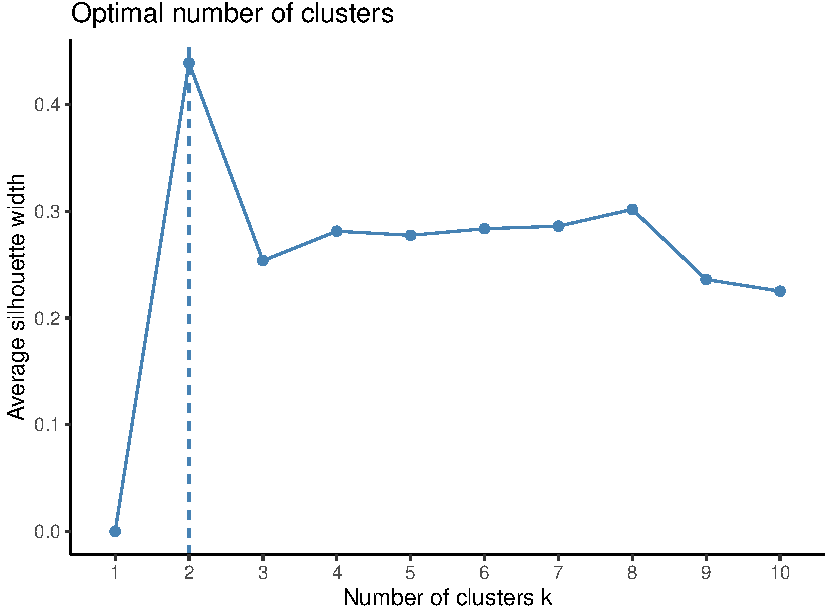
\includegraphics[width=0.8\linewidth]{03-ch3_files/figure-latex/unnamed-chunk-3-1} 

}

\caption{Plot Jumlah Cluster Metode silhouette}\label{fig:unnamed-chunk-3}
\end{figure}

Hasilnya adalah grafik yang menampilkan nilai rata-rata silhouette untuk setiap jumlah cluster. Jumlah cluster optimal ditentukan oleh nilai silhouette tertinggi, yang menunjukkan pembagian cluster terbaik dalam data.Berdasarkan plot, jumlah cluster yang disarankan adalah 2. Pada langkah berikutnya, kita akan mengelompokkan observasi ke dalam 2 cluster.

\subsection*{Eksperimen K-Medoids Clustering}\label{eksperimen-k-medoids-clustering}
\addcontentsline{toc}{subsection}{Eksperimen K-Medoids Clustering}

Berdasarkan plot hasil analisis dengan metode average silhouette, jumlah cluster optimal yang disarankan adalah 2. Oleh karena itu, dalam analisis cluster menggunakan algoritma k-medoids, kita akan menggunakan jumlah cluster \(k = 2\). Langkah ini diharapkan dapat menghasilkan pembagian cluster yang optimal dan berkualitas tinggi sesuai dengan data yang dianalisis. Berikut adalah kode untuk menjalankan algoritma k-medoids dengan \(k = 2\) menggunakan fungsi pam() dan mencetak hasilnya:

\begin{Shaded}
\begin{Highlighting}[]
\DocumentationTok{\#\# Menjalankan k{-}medoids clustering dengan k = 2}
\NormalTok{pam.res }\OtherTok{\textless{}{-}} \FunctionTok{pam}\NormalTok{(data, }\DecValTok{2}\NormalTok{)}
\end{Highlighting}
\end{Shaded}

Kode ini akan menampilkan detail hasil clustering, termasuk informasi tentang medoid, anggota cluster, dan ukuran setiap cluster.

\begin{Shaded}
\begin{Highlighting}[]
\CommentTok{\# Mencetak hasil clustering}
\FunctionTok{print}\NormalTok{(pam.res)}
\CommentTok{\#\textgreater{} Medoids:}
\CommentTok{\#\textgreater{}          ID   X1   X2   X3   X4   X5   X6   X7   X8   X9  X10}
\CommentTok{\#\textgreater{} TEGAL    28 4.78 3.91 6.70 4.84 6.35 5.82 3.00 5.99 2.98 5.98}
\CommentTok{\#\textgreater{} SEMARANG 22 1.76 2.19 1.61 2.33 1.88 1.61 0.92 0.49 2.67 1.56}
\CommentTok{\#\textgreater{} Clustering vector:}
\CommentTok{\#\textgreater{}         CILACAP        BANYUMAS     PURBALINGGA    BANJARNEGARA         KEBUMEN }
\CommentTok{\#\textgreater{}               1               1               1               1               1 }
\CommentTok{\#\textgreater{}       PURWOREJO        WONOSOBO        MAGELANG        BOYOLALI          KLATEN }
\CommentTok{\#\textgreater{}               2               2               2               2               1 }
\CommentTok{\#\textgreater{}       SUKOHARJO        WONOGIRI     KARANGANYAR          SRAGEN        GROBOGAN }
\CommentTok{\#\textgreater{}               2               2               2               2               1 }
\CommentTok{\#\textgreater{}           BLORA         REMBANG            PATI           KUDUS          JEPARA }
\CommentTok{\#\textgreater{}               2               2               2               2               1 }
\CommentTok{\#\textgreater{}         DEMAK          SEMARANG      TEMANGGUNG          KENDAL          BATANG }
\CommentTok{\#\textgreater{}               2               2               2               2               2 }
\CommentTok{\#\textgreater{}      PEKALONGAN        PEMALANG           TEGAL          BREBES   KOTA MAGELANG }
\CommentTok{\#\textgreater{}               2               1               1               1               2 }
\CommentTok{\#\textgreater{}  KOTA SURAKARTA   KOTA SALATIGA   KOTA SEMARANG KOTA PEKALONGAN      KOTA TEGAL }
\CommentTok{\#\textgreater{}               2               2               2               2               2 }
\CommentTok{\#\textgreater{} Objective function:}
\CommentTok{\#\textgreater{}    build     swap }
\CommentTok{\#\textgreater{} 4.702218 4.605625 }
\CommentTok{\#\textgreater{} }
\CommentTok{\#\textgreater{} Available components:}
\CommentTok{\#\textgreater{}  [1] "medoids"    "id.med"     "clustering" "objective"  "isolation" }
\CommentTok{\#\textgreater{}  [6] "clusinfo"   "silinfo"    "diss"       "call"       "data"}
\end{Highlighting}
\end{Shaded}

Hasil analisis k-medoids dengan \(k = 2\) menunjukkan bahwa data berhasil dikelompokkan ke dalam dua cluster. Medoid yang terpilih sebagai representasi masing-masing cluster adalah TEGAL untuk Cluster 1 dan SEMARANG untuk Cluster 2, dengan nilai atribut masing-masing ditampilkan dalam tabel. Observasi lainnya dikelompokkan berdasarkan kedekatan mereka dengan medoid, misalnya CILACAP, BANYUMAS, dan PURBALINGGA masuk ke Cluster 1, sementara PURWOREJO, WONOSOBO, dan MAGELANG masuk ke Cluster 2. Secara keseluruhan, clustering ini memberikan pembagian yang optimal dengan dua cluster yang masing-masing diwakili oleh medoid terpilih.

Untuk menambahkan klasifikasi titik (cluster) ke data asli, Anda dapat menggunakan kode berikut. Kode ini akan menggabungkan hasil klasifikasi (cluster) dari analisis k-medoids ke dalam \texttt{data} dan menampilkan 3 baris pertama dari data yang telah diperbarui:

\begin{Shaded}
\begin{Highlighting}[]
\CommentTok{\# Menambahkan klasifikasi cluster ke data asli}
\NormalTok{hasil\_cluster }\OtherTok{\textless{}{-}} \FunctionTok{cbind}\NormalTok{(data, }\AttributeTok{cluster =}\NormalTok{ pam.res}\SpecialCharTok{$}\NormalTok{cluster)}

\CommentTok{\# Menampilkan 3 baris pertama}
\FunctionTok{head}\NormalTok{(hasil\_cluster, }\AttributeTok{n =} \DecValTok{3}\NormalTok{)}
\CommentTok{\#\textgreater{}               X1   X2   X3   X4   X5   X6    X7   X8   X9  X10 cluster}
\CommentTok{\#\textgreater{} CILACAP     5.19 5.67 5.08 5.44 5.22 6.05 11.47 9.78 5.55 5.12       1}
\CommentTok{\#\textgreater{} BANYUMAS    5.71 4.47 5.18 5.51 5.02 6.21  7.39 6.96 5.98 8.22       1}
\CommentTok{\#\textgreater{} PURBALINGGA 3.30 2.19 3.80 3.13 3.73 3.34  8.71 7.41 3.21 4.65       1}
\end{Highlighting}
\end{Shaded}

Hasil dari kode ini akan menampilkan tiga baris pertama dari \texttt{data}, dengan kolom tambahan yang menunjukkan cluster tempat setiap observasi dikelompokkan. Kolom baru cluster berisi angka 1 atau 2 yang mewakili dua cluster yang terbentuk.

\subsection*{Visualisasi K-Medoids Clustering}\label{visualisasi-k-medoids-clustering}
\addcontentsline{toc}{subsection}{Visualisasi K-Medoids Clustering}

Untuk memvisualisasikan hasil pengelompokan dengan k-medoids, kita akan menggunakan fungsi \textbf{\texttt{fviz\_cluster()}} dari paket \textbf{\texttt{factoextra}}. Fungsi ini akan menghasilkan plot sebar titik data yang diwarnai sesuai dengan nomor cluster. Dalam kode ini, palet warna yang digunakan adalah \texttt{\#00AFBB} untuk cluster pertama dan \texttt{\#FC4E07} untuk cluster kedua. Elips konsentrasi ditambahkan dengan parameter ellipse.type = ``t'', yang menunjukkan distribusi data di setiap cluster. Selain itu, untuk menghindari tumpang tindih label, parameter repel = TRUE digunakan, meskipun ini dapat sedikit memperlambat proses visualisasi. Terakhir, tema plot yang klasik diterapkan dengan ggtheme = theme\_classic(), memberikan tampilan yang bersih dan sederhana pada grafik.

\begin{Shaded}
\begin{Highlighting}[]
\FunctionTok{fviz\_cluster}\NormalTok{(pam.res,}
  \AttributeTok{palette =} \FunctionTok{c}\NormalTok{(}\StringTok{"\#00AFBB"}\NormalTok{, }\StringTok{"\#FC4E07"}\NormalTok{), }\CommentTok{\# Palet warna}
  \AttributeTok{ellipse.type =} \StringTok{"t"}\NormalTok{, }\CommentTok{\# Elips konsentrasi}
  \AttributeTok{repel =} \ConstantTok{TRUE}\NormalTok{, }\CommentTok{\# Menghindari label bertumpuk (proses ini dapat sedikit lebih lambat)}
  \AttributeTok{ggtheme =} \FunctionTok{theme\_classic}\NormalTok{() }\CommentTok{\# Tema plot klasik}
\NormalTok{)}
\end{Highlighting}
\end{Shaded}

\begin{figure}[h]

{\centering \includegraphics[width=0.8\linewidth]{03-ch3_files/figure-latex/unnamed-chunk-7-1} 

}

\caption{Visualisasi Cluster K-Medoids}\label{fig:unnamed-chunk-7}
\end{figure}

\chapter{CLARA - Clustering Large Applications}\label{clra}

Analisis clustering adalah teknik statistik yang digunakan untuk
mengelompokkan objek-objek ke dalam kelompok atau kluster berdasarkan
kesamaan karakteristik. Tujuan utama dari clustering adalah untuk
memaksimalkan kesamaan dalam satu kluster dan meminimalkan kesamaan
antar kluster. Dalam konteks data besar, metode clustering tradisional
sering kali tidak efisien, sehingga diperlukan algoritma yang lebih
canggih seperti CLARA (Clustering Large Applications). CLARA dirancang
untuk menangani dataset besar dengan cara yang lebih efisien
dibandingkan dengan algoritma clustering lainnya seperti K-Means atau
K-Medoids \citep{kaufman1990finding}.

CLARA mengadopsi pendekatan sampling untuk mengatasi masalah komputasi
yang muncul saat bekerja dengan dataset besar. Algoritma ini
pertama-tama mengambil sampel dari dataset dan kemudian menerapkan
algoritma K-Medoids pada sampel tersebut untuk menemukan medoid. Setelah
itu, CLARA menghitung jarak antara setiap objek dalam dataset asli
dengan medoid yang ditemukan, dan mengelompokkan objek berdasarkan
kedekatannya dengan medoid tersebut. Proses ini diulang beberapa kali
untuk meningkatkan akurasi hasil clustering \citep{kaufman1990finding}.

Salah satu keunggulan utama dari CLARA adalah kemampuannya untuk
mengurangi waktu komputasi yang diperlukan untuk clustering dataset
besar. Dengan menggunakan teknik sampling, CLARA dapat memberikan hasil
yang representatif tanpa harus memproses seluruh dataset secara
langsung. Hal ini sangat berguna dalam aplikasi dunia nyata di mana data
sering kali sangat besar dan kompleks, seperti dalam analisis data
pelanggan, pengolahan citra, dan bioinformatika \citep{halkidi2001cluster}.

CLARA telah diterapkan dalam berbagai bidang, termasuk pemasaran,
analisis sosial, dan ilmu kesehatan. Misalnya, dalam pemasaran, CLARA
dapat digunakan untuk mengelompokkan pelanggan berdasarkan perilaku
pembelian mereka, sehingga perusahaan dapat menyesuaikan strategi
pemasaran mereka dengan lebih efektif. Di bidang kesehatan, CLARA dapat
membantu dalam pengelompokan pasien berdasarkan gejala atau respons
terhadap pengobatan, yang dapat meningkatkan perawatan pasien

Dengan meningkatnya volume data yang dihasilkan setiap hari, metode
clustering yang efisien seperti CLARA menjadi semakin penting. Algoritma
ini tidak hanya menawarkan solusi untuk masalah komputasi yang dihadapi
oleh metode clustering tradisional, tetapi juga memberikan hasil yang
dapat diandalkan dalam konteks data besar. Di masa depan, pengembangan
lebih lanjut dari algoritma ini dan integrasinya dengan teknik
pembelajaran mesin lainnya dapat membuka jalan bagi analisis data yang
lebih mendalam dan akurat.

\section{Tahapan Algoritma CLARA}\label{tahapan-algoritma-clara}

Algoritma CLARA (\emph{Clustering Large Applications}) adalah metode clustering berbasis partisi yang efisien untuk dataset besar. Berikut adalah tahapan-tahapannya:

\subsection*{1. Inisialisasi}\label{inisialisasi}
\addcontentsline{toc}{subsection}{1. Inisialisasi}

Tentukan jumlah cluster \(k\). Tentukan jumlah sampel (\emph{subsets}) yang akan diambil (\(s\)).

\subsection*{2. Pengambilan Sampel Subset Data}\label{pengambilan-sampel-subset-data}
\addcontentsline{toc}{subsection}{2. Pengambilan Sampel Subset Data}

CLARA mengambil \(s\) subset data secara acak, di mana ukuran subset data adalah \(m\). Nilai \(m\) biasanya cukup besar untuk mencakup representasi seluruh dataset.

\subsection*{3. Penerapan Algoritma PAM pada Subset Data}\label{penerapan-algoritma-pam-pada-subset-data}
\addcontentsline{toc}{subsection}{3. Penerapan Algoritma PAM pada Subset Data}

Untuk setiap subset, algoritma PAM (\emph{Partitioning Around Medoids}), Pilih \(k\) medoid awal secara acak. Tetapkan setiap data \(x_i\) ke medoid terdekat berdasarkan fungsi jarak \(d(x_i, m_j)\), di mana:
\[
     d(x_i, m_j) = \sqrt{\sum_{p=1}^P (x_{ip} - m_{jp})^2}
     \]
dengan \(P\) adalah jumlah atribut. Hitung \emph{total cost} untuk setiap medoid:
\[
     \text{Cost} = \sum_{i=1}^n \min_{j=1}^k d(x_i, m_j)
     \]
Tukar medoid dengan non-medoid secara iteratif untuk mengurangi \emph{total cost} hingga konvergen.

\subsection*{4. Pemilihan Medoid Terbaik}\label{pemilihan-medoid-terbaik}
\addcontentsline{toc}{subsection}{4. Pemilihan Medoid Terbaik}

Evaluasi semua medoid yang diperoleh dari \(s\) subset menggunakan seluruh dataset. Medoid terbaik adalah yang memiliki nilai \emph{total cost} terkecil.

\subsection*{5. Penugasan Data ke Cluster}\label{penugasan-data-ke-cluster}
\addcontentsline{toc}{subsection}{5. Penugasan Data ke Cluster}

Tetapkan seluruh data ke medoid terdekat yang dipilih pada langkah sebelumnya.

\subsection*{6. Evaluasi Kualitas Cluster}\label{evaluasi-kualitas-cluster}
\addcontentsline{toc}{subsection}{6. Evaluasi Kualitas Cluster}

Gunakan metrik evaluasi seperti \emph{silhouette coefficient}:
\[
  S(i) = \frac{b(i) - a(i)}{\max(a(i), b(i))}
  \]
di mana: \(a(i)\) adalah rata-rata jarak data \(i\) ke data lain dalam cluster yang sama. \(b(i)\) adalah rata-rata jarak data \(i\) ke data dalam cluster terdekat.

\section{Eksperimen Algoritma CLARA}\label{eksperimen-algoritma-clara}

Dalam eksperimen ini, kita akan menerapkan algoritma CLARA pada dataset yang terdiri dari dua variabel acak. Kita akan membangkitkan 500 sampel dari dua distribusi normal yang berbeda.

\subsection*{1. Memuat library yang diperlukan}\label{memuat-library-yang-diperlukan}
\addcontentsline{toc}{subsection}{1. Memuat library yang diperlukan}

Library pertama adalah \texttt{cluster}, yang digunakan untuk melakukan analisis clustering dengan berbagai algoritma, seperti PAM (\emph{Partitioning Around Medoids}) dan CLARA (\emph{Clustering Large Applications}). Dalam kasus ini, CLARA digunakan untuk mengelompokkan data besar secara efisien. Library kedua adalah \texttt{ggplot2}, yang digunakan untuk membuat visualisasi data secara estetis dan informatif. Dengan pendekatan \emph{layered grammar of graphics}, \texttt{ggplot2} memungkinkan pembuatan grafik kompleks, seperti visualisasi hasil clustering berdasarkan dua variabel dalam dataset.

\begin{Shaded}
\begin{Highlighting}[]
\FunctionTok{library}\NormalTok{(cluster)}
\FunctionTok{library}\NormalTok{(ggplot2)}
\FunctionTok{library}\NormalTok{(factoextra)}
\end{Highlighting}
\end{Shaded}

\subsection*{2. Membangkitkan data acak}\label{membangkitkan-data-acak}
\addcontentsline{toc}{subsection}{2. Membangkitkan data acak}

Data acak dibangkitkan menggunakan fungsi \texttt{rnorm()} dalam bahasa pemrograman \texttt{R}. Fungsi \texttt{rnorm()} digunakan untuk menghasilkan angka acak yang terdistribusi normal, dengan parameter pertama menunjukkan jumlah data yang ingin dibangkitkan, parameter kedua adalah rata-rata (mean), dan parameter ketiga adalah simpangan baku (standard deviation). Pada bagian pertama, dua set data acak dengan jumlah 200 titik data untuk setiap variabel \texttt{x} dan \texttt{y} dihasilkan, yang masing-masing memiliki distribusi normal dengan rata-rata 0 dan simpangan baku 8. Data ini kemudian digabungkan menggunakan fungsi \texttt{rbind()}. Pada bagian kedua, dua set data tambahan dengan jumlah 300 titik data masing-masing untuk variabel \texttt{x} dan \texttt{y} dihasilkan, dengan rata-rata 50 dan simpangan baku 8. Akhirnya, nama kolom untuk data acak tersebut ditentukan dengan fungsi \texttt{colnames()}, yaitu \texttt{x} untuk variabel pertama dan \texttt{y} untuk variabel kedua. Hasilnya adalah sebuah matriks data dua kolom yang berisi dua grup data acak dengan distribusi normal berbeda.

\begin{Shaded}
\begin{Highlighting}[]
\FunctionTok{set.seed}\NormalTok{(}\DecValTok{1234}\NormalTok{)}
\NormalTok{data }\OtherTok{\textless{}{-}} \FunctionTok{rbind}\NormalTok{(}
  \FunctionTok{cbind}\NormalTok{(}\FunctionTok{rnorm}\NormalTok{(}\DecValTok{200}\NormalTok{, }\DecValTok{0}\NormalTok{, }\DecValTok{8}\NormalTok{), }\FunctionTok{rnorm}\NormalTok{(}\DecValTok{200}\NormalTok{, }\DecValTok{0}\NormalTok{, }\DecValTok{8}\NormalTok{)),}
  \FunctionTok{cbind}\NormalTok{(}\FunctionTok{rnorm}\NormalTok{(}\DecValTok{300}\NormalTok{, }\DecValTok{50}\NormalTok{, }\DecValTok{8}\NormalTok{), }\FunctionTok{rnorm}\NormalTok{(}\DecValTok{300}\NormalTok{, }\DecValTok{50}\NormalTok{, }\DecValTok{8}\NormalTok{)))}
\FunctionTok{colnames}\NormalTok{(data) }\OtherTok{\textless{}{-}} \FunctionTok{c}\NormalTok{(}\StringTok{"x"}\NormalTok{, }\StringTok{"y"}\NormalTok{)}
\end{Highlighting}
\end{Shaded}

\subsection*{3. Visualisasi data acak}\label{visualisasi-data-acak}
\addcontentsline{toc}{subsection}{3. Visualisasi data acak}

Visualisasi data acak di atas dilakukan menggunakan paket \texttt{ggplot2} di R. Fungsi \texttt{ggplot()} digunakan untuk memulai pembuatan plot, dengan parameter \texttt{data} berisi data yang ingin divisualisasikan, dan \texttt{aes()} untuk menentukan hubungan antara variabel-variabel yang akan diplot, yaitu \texttt{x} dan \texttt{y}. Selanjutnya, fungsi \texttt{geom\_point()} digunakan untuk membuat grafik titik (scatter plot), dengan argumen \texttt{alpha\ =\ 0.5} untuk memberikan tingkat transparansi pada titik-titik, sehingga memungkinkan visualisasi yang lebih jelas ketika titik-titik saling tumpang tindih. Judul plot diatur menggunakan \texttt{labs()} dengan parameter \texttt{title}, \texttt{x}, dan \texttt{y} untuk memberikan label pada plot dan sumbu X serta Y. Terakhir, \texttt{theme\_minimal()} diterapkan untuk memberikan tampilan plot yang bersih dan sederhana. Hasil dari kode ini adalah visualisasi data acak dalam bentuk scatter plot dengan dua variabel, menunjukkan dua kelompok data dengan distribusi normal yang berbeda.

\begin{figure}[h]

{\centering \includegraphics[width=0.8\linewidth]{04-ch4_files/figure-latex/unnamed-chunk-4-1} 

}

\caption{Visualisasi Data}\label{fig:unnamed-chunk-4}
\end{figure}

\subsection*{4. Mencari Jumlah CLluster Optimal}\label{mencari-jumlah-clluster-optimal}
\addcontentsline{toc}{subsection}{4. Mencari Jumlah CLluster Optimal}

Visualisasi jumlah klaster yang optimal dilakukan menggunakan metode silhouette dengan paket \texttt{cluster} dan \texttt{factoextra} di R. Fungsi \texttt{fviz\_nbclust()} digunakan untuk menilai jumlah klaster terbaik berdasarkan metode yang dipilih, dalam hal ini menggunakan algoritma \texttt{clara} (Clustering Large Applications). Metode silhouette mengukur seberapa baik setiap objek dipisahkan dari klaster lain, dengan nilai yang lebih tinggi menunjukkan pemisahan yang lebih baik. Parameter \texttt{method\ =\ "silhouette"} mengindikasikan bahwa visualisasi menggunakan metode tersebut. Hasilnya akan memperlihatkan grafik yang menggambarkan nilai rata-rata silhouette untuk berbagai jumlah klaster. Terakhir, fungsi \texttt{theme\_classic()} diterapkan untuk memberikan tampilan plot yang bersih dan sederhana. Grafik ini dapat membantu dalam menentukan jumlah klaster yang paling sesuai dengan data berdasarkan evaluasi kualitas pemisahan antar klaster.

\begin{Shaded}
\begin{Highlighting}[]
\FunctionTok{fviz\_nbclust}\NormalTok{(data, clara, }\AttributeTok{method =} \StringTok{"silhouette"}\NormalTok{)}\SpecialCharTok{+}
\FunctionTok{theme\_classic}\NormalTok{()}
\end{Highlighting}
\end{Shaded}

\begin{figure}[h]

{\centering \includegraphics[width=0.8\linewidth]{04-ch4_files/figure-latex/unnamed-chunk-5-1} 

}

\caption{Jumlah Cluster Optimal}\label{fig:unnamed-chunk-5}
\end{figure}

\subsection*{5. Menjalankan CLARA}\label{menjalankan-clara}
\addcontentsline{toc}{subsection}{5. Menjalankan CLARA}

Algoritma CLARA (Clustering Large Applications) digunakan untuk melakukan klasterisasi data dengan jumlah klaster yang ditentukan sebanyak 2, yang ditetapkan melalui parameter \texttt{k\ =\ 2}. Fungsi \texttt{clara()} dari paket \texttt{cluster} di R dirancang untuk melakukan klasterisasi pada dataset besar dengan cara mengacak sampel data untuk mempercepat proses klasterisasi. Parameter \texttt{samples\ =\ 5} menunjukkan bahwa lima sampel data acak akan diambil untuk setiap iterasi klasterisasi. Hasil dari klasterisasi ini disimpan dalam objek \texttt{clara\_result}, yang berisi informasi tentang klaster yang terbentuk, termasuk elemen-elemen data yang termasuk dalam setiap klaster dan pusat klaster.

\begin{Shaded}
\begin{Highlighting}[]
\NormalTok{clara\_result }\OtherTok{\textless{}{-}} \FunctionTok{clara}\NormalTok{(data, }\AttributeTok{k =} \DecValTok{2}\NormalTok{, }\AttributeTok{samples =} \DecValTok{5}\NormalTok{)}
\end{Highlighting}
\end{Shaded}

\subsection*{6. Evaluasi hasil}\label{evaluasi-hasil}
\addcontentsline{toc}{subsection}{6. Evaluasi hasil}

\texttt{print(clara\_result)} digunakan untuk menampilkan hasil dari proses klasterisasi yang dilakukan dengan algoritma CLARA. Setelah data dikelompokkan menjadi dua klaster menggunakan parameter \texttt{k\ =\ 2}, hasil ini memberikan informasi tentang bagaimana data dibagi. Secara spesifik, hasil tersebut akan menunjukkan anggota klaster, yaitu data mana yang tergabung dalam setiap klaster, serta pusat klaster, yang menggambarkan titik tengah dari masing-masing klaster. Selain itu, hasil ini juga dapat mencakup ukuran atau indeks kualitas klaster, yang digunakan untuk mengevaluasi sejauh mana klaster-klaster tersebut terpisah dengan baik satu sama lain. Dengan demikian, fungsi \texttt{print(clara\_result)} memberikan gambaran yang jelas tentang hasil klasterisasi dan seberapa baik data dapat dikelompokkan dalam dua klaster.

\begin{Shaded}
\begin{Highlighting}[]
\FunctionTok{print}\NormalTok{(clara\_result)}
\CommentTok{\#\textgreater{} Call:     clara(x = data, k = 2, samples = 5) }
\CommentTok{\#\textgreater{} Medoids:}
\CommentTok{\#\textgreater{}               x         y}
\CommentTok{\#\textgreater{} [1,] {-}0.5495492  2.458514}
\CommentTok{\#\textgreater{} [2,] 47.5964047 50.892735}
\CommentTok{\#\textgreater{} Objective function:   9.9971}
\CommentTok{\#\textgreater{} Clustering vector:    int [1:500] 1 1 1 1 1 1 1 1 1 1 1 1 1 1 1 1 1 1 ...}
\CommentTok{\#\textgreater{} Cluster sizes:            200 300 }
\CommentTok{\#\textgreater{} Best sample:}
\CommentTok{\#\textgreater{}  [1]   6  45  51  67  75  85  90  94  97 110 111 160 168 170 176 181 201 219 249}
\CommentTok{\#\textgreater{} [20] 260 264 275 296 304 317 319 337 361 362 369 370 374 379 397 398 411 420 422}
\CommentTok{\#\textgreater{} [39] 424 436 448 458 465 489}
\CommentTok{\#\textgreater{} }
\CommentTok{\#\textgreater{} Available components:}
\CommentTok{\#\textgreater{}  [1] "sample"     "medoids"    "i.med"      "clustering" "objective" }
\CommentTok{\#\textgreater{}  [6] "clusinfo"   "diss"       "call"       "silinfo"    "data"}
\end{Highlighting}
\end{Shaded}

\subsection*{7. Visualisasi Hasil Cluster}\label{visualisasi-hasil-cluster}
\addcontentsline{toc}{subsection}{7. Visualisasi Hasil Cluster}

Visualisasi silhouette digunakan untuk mengevaluasi kualitas klaster yang dihasilkan oleh algoritma CLARA. Fungsi \texttt{silhouette()} menghitung nilai silhouette untuk setiap titik data berdasarkan klaster yang telah ditetapkan (\texttt{clara\_result\$clustering}) dan jarak antar data (\texttt{dist(data)}). Nilai silhouette mengukur sejauh mana setiap titik data berada dalam klaster yang benar, dengan nilai mendekati +1 menunjukkan bahwa titik data tersebut sangat cocok dengan klasternya, sedangkan nilai mendekati -1 menunjukkan bahwa titik tersebut lebih cocok dengan klaster lain.

Selanjutnya, fungsi \texttt{plot(sil,\ border\ =\ NA)} digunakan untuk menghasilkan plot visualisasi dari hasil silhouette. Parameter \texttt{border\ =\ NA} menghilangkan batas pada setiap segmen plot untuk memberikan tampilan yang lebih bersih. Hasil visualisasi ini memberikan gambaran tentang kualitas pemisahan antar klaster, dengan tinggi nilai silhouette menunjukkan klasterisasi yang baik.

\begin{Shaded}
\begin{Highlighting}[]
\NormalTok{sil }\OtherTok{\textless{}{-}} \FunctionTok{silhouette}\NormalTok{(clara\_result}\SpecialCharTok{$}\NormalTok{clustering, }\FunctionTok{dist}\NormalTok{(data))}
\FunctionTok{plot}\NormalTok{(sil, }\AttributeTok{border =} \ConstantTok{NA}\NormalTok{)}
\end{Highlighting}
\end{Shaded}

\begin{figure}[h]

{\centering \includegraphics[width=0.8\linewidth]{04-ch4_files/figure-latex/unnamed-chunk-8-1} 

}

\caption{Visualisasi silhouette}\label{fig:unnamed-chunk-8}
\end{figure}

Kode ini menggunakan fungsi \texttt{fviz\_cluster()} untuk memvisualisasikan hasil klasterisasi yang dilakukan dengan algoritma CLARA. Visualisasi ini menampilkan titik-titik data yang dikelompokkan berdasarkan klaster yang telah ditentukan, dengan dua klaster yang masing-masing diberi warna berbeda menggunakan palet warna \texttt{\#00AFBB} dan \texttt{\#FC4E07}. Elips konsentrasi (\texttt{ellipse.type\ =\ "t"}) ditambahkan di sekitar setiap klaster, yang menunjukkan area distribusi data dalam klaster tersebut, memberikan gambaran tentang seberapa padat atau tersebarnya data. Dengan parameter \texttt{geom\ =\ "point"}, visualisasi ini menampilkan titik-titik data, dan ukuran titik diatur menggunakan \texttt{pointsize\ =\ 1}. Tema klasik (\texttt{theme\_classic()}) diterapkan untuk memberikan tampilan plot yang bersih dan sederhana. Hasil dari kode ini adalah visualisasi yang jelas tentang pembagian data ke dalam dua klaster dengan warna yang berbeda, serta gambaran tentang penyebaran data di dalam setiap klaster.

\begin{Shaded}
\begin{Highlighting}[]
\FunctionTok{fviz\_cluster}\NormalTok{(clara\_result,}
\AttributeTok{palette =} \FunctionTok{c}\NormalTok{(}\StringTok{"\#00AFBB"}\NormalTok{, }\StringTok{"\#FC4E07"}\NormalTok{), }\CommentTok{\# color palette}
\AttributeTok{ellipse.type =} \StringTok{"t"}\NormalTok{, }\CommentTok{\# Concentration ellipse}
\AttributeTok{geom =} \StringTok{"point"}\NormalTok{, }\AttributeTok{pointsize =} \DecValTok{1}\NormalTok{,}
\AttributeTok{ggtheme =} \FunctionTok{theme\_classic}\NormalTok{()}
\NormalTok{)}
\end{Highlighting}
\end{Shaded}

\begin{figure}[h]

{\centering \includegraphics[width=0.8\linewidth]{04-ch4_files/figure-latex/unnamed-chunk-9-1} 

}

\caption{Visualisasi Hasil Cluster}\label{fig:unnamed-chunk-9}
\end{figure}

\chapter{Algoritma K-Modes}\label{kmods}

Algoritma K-Modes merupakan salah satu metode dalam analisis clustering
yang dirancang khusus untuk mengelompokkan data kategorik. Berbeda
dengan algoritma K-Means yang hanya dapat digunakan untuk data numerik,
K-Modes mengatasi keterbatasan ini dengan menggunakan modus sebagai
pusat cluster. Hal ini memungkinkan K-Modes untuk menangani data yang
memiliki atribut kategorik, seperti jenis kelamin, status perkawinan,
atau kategori produk, yang sering dijumpai dalam berbagai aplikasi
analisis data \citep{handayani2020}.

Proses kerja algoritma K-Modes mirip dengan K-Means, di mana algoritma
ini juga memerlukan penentuan jumlah cluster (\(k\)) sebelum proses
clustering dimulai. K-Modes melakukan inisialisasi centroid dengan
memilih modus dari setiap atribut dalam cluster. Selanjutnya, algoritma
ini menghitung jarak antara data dan centroid menggunakan metode yang
disebut ``dissimilarity measure,'' yang mengukur seberapa berbeda dua data
berdasarkan atribut kategorik \citep{buulolo2020}.

Salah satu keunggulan K-Modes adalah kemampuannya untuk mengatasi data
yang mengandung noise atau outlier. Dalam konteks data kategorik,
outlier dapat mempengaruhi hasil clustering secara signifikan. K-Modes
menggunakan pendekatan yang lebih robust dengan memfokuskan pada modus,
sehingga hasil clustering menjadi lebih stabil dan representatif
\citep{hardandy2017}.

Implementasi K-Modes dalam R dapat dilakukan dengan menggunakan paket
seperti klaR dan cluster, yang menyediakan fungsi-fungsi yang diperlukan
untuk melakukan clustering. Dengan menggunakan dataset yang sesuai,
pengguna dapat dengan mudah menerapkan algoritma ini untuk mendapatkan
insight yang berharga dari data kategorik yang dimiliki
\citep{widyakusuma2024}.

Dalam bab ini, kita akan membahas lebih dalam mengenai langkah-langkah
implementasi algoritma K-Modes, termasuk pemilihan jumlah cluster yang
optimal, serta analisis hasil clustering yang diperoleh. Dengan
pemahaman yang baik tentang algoritma ini, diharapkan pembaca dapat
menerapkan K-Modes dalam berbagai konteks analisis data yang relevan.

\section{Tahapan Algoritma K-Modes}\label{tahapan-algoritma-k-modes}

\subsection*{1. Inisialisasi}\label{inisialisasi-1}
\addcontentsline{toc}{subsection}{1. Inisialisasi}

Tentukan jumlah cluster \(k\). Pilih \(k\) modus dari dataset sebagai centroid awal. Modus adalah nilai yang paling sering muncul dalam setiap atribut kategorik.

\subsection*{2. Pengelompokan}\label{pengelompokan}
\addcontentsline{toc}{subsection}{2. Pengelompokan}

Untuk setiap data point, hitung jarak dissimilarity ke setiap centroid. Dalam K-Modes, jarak dissimilarity dihitung menggunakan rumus berikut:

\[
d(x_i, c_j) = \sum_{k=1}^{n} \delta(x_{ik}, c_{jk})
\]

di mana: \(d(x_i, c_j)\) adalah jarak dissimilarity antara data point \(x_i\) dan centroid \(c_j\). \(\delta(x_{ik}, c_{jk})\) adalah fungsi yang mengembalikan 0 jika \(x_{ik} = c_{jk}\) (nilai sama) dan 1 jika \(x_{ik} \neq c_{jk}\) (nilai berbeda). \(n\) adalah jumlah atribut.

\subsection*{3. Penugasan Cluster}\label{penugasan-cluster-1}
\addcontentsline{toc}{subsection}{3. Penugasan Cluster}

Setiap data point \(x_i\) ditugaskan ke cluster dengan centroid terdekat (dengan jarak dissimilarity terkecil).

\subsection*{4. Update Centroid}\label{update-centroid}
\addcontentsline{toc}{subsection}{4. Update Centroid}

Setelah semua data point ditugaskan ke cluster, hitung ulang centroid untuk setiap cluster dengan mengambil modus dari setiap atribut dalam cluster tersebut. Modus dapat dihitung dengan:

\[
c_j = \text{modus}(X_j)
\]

di mana \(X_j\) adalah himpunan data point yang ditugaskan ke cluster \(j\).

\subsection*{5. Kondisi Berhenti}\label{kondisi-berhenti}
\addcontentsline{toc}{subsection}{5. Kondisi Berhenti}

Ulangi langkah 2 hingga 4 sampai tidak ada perubahan dalam penugasan cluster atau sampai jumlah iterasi maksimum tercapai.

\subsection*{Penjelasan Tambahan}\label{penjelasan-tambahan}
\addcontentsline{toc}{subsection}{Penjelasan Tambahan}

\begin{itemize}
\tightlist
\item
  \textbf{Centroid}: Dalam konteks K-Modes, centroid adalah modus dari atribut-atribut dalam cluster. Ini berbeda dengan K-Means, di mana centroid adalah rata-rata dari atribut numerik.
\item
  \textbf{Iterasi}: Proses ini diulang hingga tidak ada perubahan dalam penugasan cluster, yang menunjukkan bahwa algoritma telah konvergen.
\end{itemize}

\section{Eksperimen Algoritma K-Modes}\label{eksperimen-algoritma-k-modes}

\subsection*{1. Memuat library yang diperlukan}\label{memuat-library-yang-diperlukan-1}
\addcontentsline{toc}{subsection}{1. Memuat library yang diperlukan}

Algoritma k-modes adalah salah satu metode clustering yang dirancang khusus untuk menangani data kategorikal. Di \texttt{R}, algoritma ini dapat diimplementasikan dengan menggunakan library \texttt{Klar}, yang menyediakan fungsi bawaan untuk k-modes. Selain itu, library \texttt{MASS} sering digunakan untuk mendukung manipulasi data atau keperluan lainnya dalam analisis clustering.

\begin{Shaded}
\begin{Highlighting}[]
\FunctionTok{library}\NormalTok{(klaR)}
\FunctionTok{library}\NormalTok{(MASS)}
\end{Highlighting}
\end{Shaded}

\subsection*{2. Persiapan Dataset}\label{persiapan-dataset}
\addcontentsline{toc}{subsection}{2. Persiapan Dataset}

Package \textbf{readr} menyiapkan fungsi \href{https://readr.tidyverse.org/reference/read_delim.html}{\texttt{read\_csv()}} untuk import data dari file CSV. Pada kasus ini digunakan data \href{https://github.com/dedenistiawan/dataset}{Daerah Aliran Sungai} (DAS).

\begin{Shaded}
\begin{Highlighting}[]
\FunctionTok{library}\NormalTok{ (readr)}
\NormalTok{urlfile }\OtherTok{=} \StringTok{"https://raw.githubusercontent.com/dedenistiawan/Dataset/main/Dataset\%20DAS.csv"}
\NormalTok{data}\OtherTok{\textless{}{-}}\FunctionTok{read\_csv}\NormalTok{(}\FunctionTok{url}\NormalTok{(urlfile))}
\end{Highlighting}
\end{Shaded}

\begin{table}

\caption{\label{tab:nice-tab-1}Data Daerah Aliran Sungai}
\centering
\begin{tabular}[t]{llll}
\toprule
PRODUKTIVITAS & KEMIRINGAN LERENG & TINGKAT EROSI & MANAJEMEN LAHAN\\
\midrule
Sangat Tinggi & Datar & Berat & Baik\\
Sangat Tinggi & Datar & Sangat Berat & Baik\\
Sangat Rendah & Datar & Sedang & Buruk\\
Sangat Rendah & Datar & Sedang & Buruk\\
Sangat Tinggi & Datar & Sedang & Baik\\
\addlinespace
Sangat Tinggi & Datar & Sedang & Baik\\
Sangat Tinggi & Datar & Sedang & Baik\\
Sangat Rendah & Datar & Sedang & Buruk\\
Sangat Tinggi & Datar & Sedang & Baik\\
Sangat Tinggi & Datar & Sedang & Baik\\
\bottomrule
\end{tabular}
\end{table}

\subsection*{3. Memeriksa Missing value}\label{memeriksa-missing-value-1}
\addcontentsline{toc}{subsection}{3. Memeriksa Missing value}

Untuk memeriksa keberadaan \textbf{missing value} dalam dataset, kita dapat menggunakan fungsi \textbf{\texttt{is.na()}} yang mengidentifikasi elemen dengan nilai yang hilang (NA). Dalam kasus ini, perintah \textbf{\texttt{colSums(is.na(data))}} digunakan untuk menghitung jumlah nilai yang hilang pada setiap kolom dalam dataset. Fungsi \textbf{\texttt{is.na(data)}} menghasilkan matriks logika yang menunjukkan posisi nilai yang hilang, di mana nilai \texttt{TRUE} menandakan keberadaan missing value. Selanjutnya, \textbf{\texttt{colSums()}} menjumlahkan nilai \texttt{TRUE} tersebut untuk setiap kolom, sehingga memberikan informasi tentang jumlah nilai yang hilang per kolom. Dengan hasil ini, pengguna dapat dengan mudah mengidentifikasi kolom yang memerlukan penanganan lebih lanjut, seperti imputasi atau penghapusan data.

\begin{Shaded}
\begin{Highlighting}[]
\FunctionTok{colSums}\NormalTok{(}\FunctionTok{is.na}\NormalTok{(data))}
\CommentTok{\#\textgreater{}     PRODUKTIVITAS KEMIRINGAN LERENG     TINGKAT EROSI   MANAJEMEN LAHAN }
\CommentTok{\#\textgreater{}                 0                 0                 0                 0}
\end{Highlighting}
\end{Shaded}

\subsection*{3. Menjalankan K-Modes}\label{menjalankan-k-modes}
\addcontentsline{toc}{subsection}{3. Menjalankan K-Modes}

Proses diawali dengan menjalankan fungsi \textbf{\texttt{kmodes()}}, di mana dataset dibagi ke dalam 3 cluster dengan parameter iterasi maksimum sebesar 10 dan tanpa pembobotan (parameter \texttt{weighted\ =\ FALSE}). Hasil clustering disimpan dalam variabel \textbf{\texttt{cluster.results}}, yang mencakup informasi tentang mode dari setiap cluster dan label cluster untuk setiap baris data. Selanjutnya, hasil cluster tersebut ditambahkan sebagai kolom baru ke dataset asli menggunakan fungsi \textbf{\texttt{cbind()}}, menghasilkan data frame baru yang mencakup informasi label cluster untuk setiap data. Dengan demikian, dataset hasil clustering ini dapat digunakan untuk analisis lebih lanjut, seperti mengidentifikasi pola atau karakteristik di dalam setiap cluster.

\begin{Shaded}
\begin{Highlighting}[]
\NormalTok{kmodes\_result }\OtherTok{\textless{}{-}} \FunctionTok{kmodes}\NormalTok{(data , }\DecValTok{3}\NormalTok{, }\AttributeTok{iter.max =} \DecValTok{10}\NormalTok{, }\AttributeTok{weighted =} \ConstantTok{FALSE}\NormalTok{ )}
\NormalTok{cluster.output }\OtherTok{\textless{}{-}} \FunctionTok{cbind}\NormalTok{(data ,kmodes\_result}\SpecialCharTok{$}\NormalTok{cluster)}
\end{Highlighting}
\end{Shaded}

\subsection*{4. Menyimpan Hasil Cluster}\label{menyimpan-hasil-cluster}
\addcontentsline{toc}{subsection}{4. Menyimpan Hasil Cluster}

Fungsi \textbf{\texttt{write.csv()}} digunakan untuk mengekspor data frame \textbf{\texttt{cluster.output}}, yang berisi dataset asli beserta label cluster hasil algoritma k-modes, ke file bernama \emph{``kmodes clusters.csv''}. Parameter \textbf{\texttt{row.names\ =\ TRUE}} memastikan bahwa nama baris dari data frame akan disertakan dalam file CSV yang dihasilkan. File ini disimpan di direktori kerja R saat ini dan dapat diakses menggunakan perangkat lunak spreadsheet seperti Microsoft Excel atau diimpor kembali ke R untuk analisis lebih lanjut.

\begin{Shaded}
\begin{Highlighting}[]
\FunctionTok{write.csv}\NormalTok{(cluster.output, }\AttributeTok{file =} \StringTok{"kmodes clusters.csv"}\NormalTok{, }\AttributeTok{row.names =} \ConstantTok{TRUE}\NormalTok{)}
\end{Highlighting}
\end{Shaded}

\part{Pendekatan Hirarki}\label{part-pendekatan-hirarki}

\chapter{Metode Cluster Hirarki}\label{HC}

Hierarchical clustering adalah salah satu metode analisis klaster yang digunakan untuk mengelompokkan data berdasarkan kemiripan atau jarak antar objek. Berbeda dengan metode klaster lainnya seperti K-Means, hierarchical clustering tidak memerlukan jumlah klaster yang telah ditentukan sebelumnya. Prosesnya dimulai dengan setiap objek dianggap sebagai klaster tersendiri, yang kemudian digabungkan secara bertahap hingga membentuk satu klaster besar atau, sebaliknya, dengan memisahkan satu klaster besar menjadi klaster-klaster kecil. Teknik ini memberikan fleksibilitas dalam mengeksplorasi struktur data tanpa asumsi awal yang ketat \citep{everitt2011cluster} .

Hierarchical clustering terdiri dari dua pendekatan utama, yaitu agglomerative dan divisive. Pendekatan agglomerative, yang lebih umum digunakan, memulai dengan setiap objek sebagai klaster individu dan secara iteratif menggabungkan klaster yang paling mirip. Sebaliknya, divisive memulai dengan satu klaster besar yang mencakup semua objek, kemudian secara bertahap membagi klaster menjadi klaster-klaster yang lebih kecil. Kedua pendekatan ini menggunakan matriks jarak untuk mengukur kedekatan antara objek atau klaster, dengan berbagai metrik seperti jarak Euclidean atau korelasi Pearson \citep{hartigan1979algorithm}.

Salah satu keuntungan utama hierarchical clustering adalah kemampuannya untuk menghasilkan dendrogram, yaitu representasi visual yang menunjukkan hubungan hierarkis antara klaster. Dendrogram memungkinkan pengguna untuk memutuskan jumlah klaster yang optimal dengan memotong pohon pada level tertentu. Selain itu, hierarchical clustering juga bermanfaat untuk mengeksplorasi data yang tidak memiliki struktur klaster yang jelas atau memiliki pola yang kompleks \citep{sokal1958statistical}.

Namun, hierarchical clustering memiliki beberapa keterbatasan. Metode ini cenderung kurang efisien untuk dataset besar karena kompleksitas komputasinya yang tinggi. Selain itu, keputusan penggabungan atau pemisahan pada tahap awal bersifat permanen, sehingga kesalahan awal dapat memengaruhi hasil akhir. Oleh karena itu, pemilihan metrik jarak dan metode penggabungan menjadi faktor krusial dalam menghasilkan klaster yang relevan dan bermakna \citep{jain2010}.

\section{Tahapan Agglomerative Clustering}\label{tahapan-agglomerative-clustering}

Agglomerative Clustering adalah salah satu metode dalam hierarchical clustering yang menggunakan pendekatan bottom-up. Metode ini mengelompokkan data dengan cara menggabungkan cluster yang paling dekat satu sama lain hingga semua data tergabung dalam satu cluster atau hingga jumlah cluster yang diinginkan tercapai.

\subsection*{1. Inisialisasi}\label{inisialisasi-2}
\addcontentsline{toc}{subsection}{1. Inisialisasi}

Setiap objek (data point) dianggap sebagai satu cluster terpisah. Jika ada \(n\) objek, maka akan ada \(n\) cluster pada awalnya.

\subsection*{2. Menghitung Jarak}\label{menghitung-jarak}
\addcontentsline{toc}{subsection}{2. Menghitung Jarak}

Hitung jarak antara semua pasangan cluster. Jarak ini dapat dihitung menggunakan berbagai metrik, seperti Euclidean, Manhattan, atau Cosine. Untuk dua titik \(A(x_1, y_1)\) dan \(B(x_2, y_2)\), jarak Euclidean dapat dihitung dengan rumus:

\[
d(A, B) = \sqrt{(x_2 - x_1)^2 + (y_2 - y_1)^2}
\]

\subsection*{3. Menggabungkan Cluster}\label{menggabungkan-cluster}
\addcontentsline{toc}{subsection}{3. Menggabungkan Cluster}

Temukan dua cluster terdekat (dengan jarak terkecil) dan gabungkan mereka menjadi satu cluster baru. Proses ini mengurangi jumlah cluster sebanyak satu.

\subsection*{4. Memperbarui Jarak}\label{memperbarui-jarak}
\addcontentsline{toc}{subsection}{4. Memperbarui Jarak}

Setelah penggabungan, perbarui matriks jarak untuk mencerminkan jarak antara cluster baru dan cluster lainnya. Ada beberapa metode untuk memperbarui jarak, termasuk:

\begin{itemize}
\item
  \textbf{Single Linkage}: Jarak minimum antara anggota dua cluster.

  \[
  d(A, B) = \min \{ d(a, b) \,|\, a \in A, b \in B \}
  \]
\item
  \textbf{Complete Linkage}: Jarak maksimum antara anggota dua cluster.

  \[
  d(A, B) = \max \{ d(a, b) \,|\, a \in A, b \in B \}
  \]
\item
  \textbf{Average Linkage}: Rata-rata jarak antara semua pasangan anggota dari dua cluster.

  \[
  d(A, B) = \frac{1}{|A| \cdot |B|} \sum_{a \in A} \sum_{b \in B} d(a, b)
  \]
\item
  \textbf{Ward's Method}: Menghitung jarak berdasarkan peningkatan varians yang dihasilkan dari penggabungan dua cluster.

  \[
  d(A, B) = \sqrt{\frac{n_A n_B}{n_A + n_B} \cdot d^2(A, B)}
  \]

  di mana \(n_A\) dan \(n_B\) adalah jumlah anggota dalam cluster \(A\) dan \(B\).
\end{itemize}

\subsection*{5. Ulangi Proses}\label{ulangi-proses}
\addcontentsline{toc}{subsection}{5. Ulangi Proses}

Ulangi langkah 3 dan 4 hingga semua objek tergabung dalam satu cluster atau hingga jumlah cluster yang diinginkan tercapai.

\subsection*{6. Membuat Dendrogram}\label{membuat-dendrogram}
\addcontentsline{toc}{subsection}{6. Membuat Dendrogram}

Setelah semua penggabungan selesai, buat dendrogram untuk memvisualisasikan proses penggabungan cluster. Dendrogram menunjukkan hubungan antar cluster dan dapat digunakan untuk menentukan jumlah cluster yang optimal dengan memotong dendrogram pada ketinggian tertentu.

\subsection*{Kesimpulan}\label{kesimpulan}
\addcontentsline{toc}{subsection}{Kesimpulan}

Agglomerative Clustering adalah metode yang efektif untuk mengelompokkan data berdasarkan kesamaan. Dengan mengikuti tahapan di atas, Anda dapat menerapkan teknik ini untuk berbagai aplikasi analisis data. Pastikan untuk memilih metrik jarak dan metode penggabungan yang sesuai dengan karakteristik data Anda untuk mendapatkan hasil yang optimal.

\section{Eksperimen Agglomerative Clustering}\label{eksperimen-agglomerative-clustering}

\begin{Shaded}
\begin{Highlighting}[]
\FunctionTok{library}\NormalTok{ (readr)}
\NormalTok{urlfile }\OtherTok{=} \StringTok{"https://bit.ly/3VO3kRE"}
\NormalTok{data}\OtherTok{\textless{}{-}}\FunctionTok{read.csv}\NormalTok{(}\FunctionTok{url}\NormalTok{(urlfile), }\AttributeTok{row.names =} \StringTok{"Kabupaten"}\NormalTok{)}
\end{Highlighting}
\end{Shaded}

\begin{table}

\caption{\label{tab:nice-tab-2}Basis Data Terpadu Jawa Tengah}
\centering
\begin{tabular}[t]{lrrrrrrrrrr}
\toprule
  & X1 & X2 & X3 & X4 & X5 & X6 & X7 & X8 & X9 & X10\\
\midrule
CILACAP & 5.19 & 5.67 & 5.08 & 5.44 & 5.22 & 6.05 & 11.47 & 9.78 & 5.55 & 5.12\\
BANYUMAS & 5.71 & 4.47 & 5.18 & 5.51 & 5.02 & 6.21 & 7.39 & 6.96 & 5.98 & 8.22\\
PURBALINGGA & 3.30 & 2.19 & 3.80 & 3.13 & 3.73 & 3.34 & 8.71 & 7.41 & 3.21 & 4.65\\
BANJARNEGARA & 2.73 & 2.34 & 3.76 & 2.80 & 2.57 & 2.99 & 3.31 & 5.45 & 4.21 & 6.05\\
KEBUMEN & 4.17 & 2.55 & 3.26 & 4.16 & 3.15 & 4.15 & 4.30 & 9.29 & 4.61 & 4.34\\
\addlinespace
PURWOREJO & 1.87 & 2.12 & 1.48 & 3.05 & 1.78 & 1.83 & 5.00 & 4.90 & 3.12 & 2.09\\
WONOSOBO & 2.13 & 1.95 & 3.00 & 1.78 & 1.62 & 2.06 & 0.45 & 2.32 & 3.57 & 0.84\\
MAGELANG & 3.95 & 3.01 & 4.22 & 4.15 & 3.01 & 3.64 & 1.44 & 3.35 & 5.69 & 3.67\\
BOYOLALI & 2.19 & 3.07 & 1.61 & 2.74 & 2.11 & 1.82 & 1.71 & 2.34 & 3.41 & 1.55\\
KLATEN & 3.84 & 5.15 & 1.93 & 4.64 & 4.04 & 3.78 & 8.71 & 4.45 & 3.99 & 3.09\\
\bottomrule
\end{tabular}
\end{table}

\subsection*{Standarisasi Data}\label{standarisasi-data}
\addcontentsline{toc}{subsection}{Standarisasi Data}

Sebelum melakukan analisis clustering, penting untuk menstandarisasi data agar setiap fitur memiliki skala yang sama. Standarisasi membantu menghindari bias yang mungkin muncul akibat perbedaan skala antar fitur, yang dapat mempengaruhi hasil analisis, terutama dalam pengukuran jarak.

Dalam R, kita dapat menggunakan fungsi \texttt{scale()} untuk menstandarisasi dataset. Fungsi ini mengubah setiap fitur dalam dataset sehingga memiliki rata-rata 0 dan deviasi standar 1. Proses ini dilakukan dengan cara mengurangi rata-rata dari setiap nilai dan membaginya dengan deviasi standar fitur tersebut.

\begin{Shaded}
\begin{Highlighting}[]
\CommentTok{\# Standarisasi Data}
\NormalTok{df }\OtherTok{\textless{}{-}} \FunctionTok{scale}\NormalTok{(data)}
\end{Highlighting}
\end{Shaded}

\begin{table}

\caption{\label{tab:nice-tab-1}Data Hasil Standarisasi}
\centering
\begin{tabular}[t]{lrrrrrrrrrr}
\toprule
  & X1 & X2 & X3 & X4 & X5 & X6 & X7 & X8 & X9 & X10\\
\midrule
CILACAP & 1.4450108 & 1.6357957 & 1.0041319 & 1.6983202 & 1.3694832 & 1.7177332 & 3.2150170 & 2.4732171 & 1.5722235 & 0.8644476\\
BANYUMAS & 1.7671470 & 0.9380866 & 1.0492817 & 1.7443527 & 1.2535376 & 1.8038274 & 1.6920805 & 1.4657198 & 1.8233322 & 2.0488467\\
PURBALINGGA & 0.2741697 & -0.3875608 & 0.4262142 & 0.1792452 & 0.5056885 & 0.2595125 & 2.1847953 & 1.6264906 & 0.2057255 & 0.6848774\\
BANJARNEGARA & -0.0789411 & -0.3003472 & 0.4081543 & -0.0377655 & -0.1667960 & 0.0711815 & 0.1691441 & 0.9262442 & 0.7896990 & 1.2197673\\
KEBUMEN & 0.8131283 & -0.1782481 & 0.1824052 & 0.8565817 & 0.1694462 & 0.6953645 & 0.5386801 & 2.2981555 & 1.0232884 & 0.5664375\\
\addlinespace
PURWOREJO & -0.6117047 & -0.4282605 & -0.6212614 & 0.1266366 & -0.6247812 & -0.5530016 & 0.7999682 & 0.7297465 & 0.1531679 & -0.2932070\\
WONOSOBO & -0.4506367 & -0.5271026 & 0.0650157 & -0.7085259 & -0.7175376 & -0.4292411 & -0.8984045 & -0.1920063 & 0.4159560 & -0.7707873\\
MAGELANG & 0.6768400 & 0.0892071 & 0.6158435 & 0.8500056 & 0.0882843 & 0.4209392 & -0.5288685 & 0.1759803 & 1.6539798 & 0.3104545\\
BOYOLALI & -0.4134671 & 0.1240926 & -0.5625667 & -0.0772220 & -0.4334709 & -0.5583825 & -0.4280859 & -0.1848610 & 0.3225202 & -0.4995217\\
KLATEN & 0.6086958 & 1.3334551 & -0.4180873 & 1.1722336 & 0.6854041 & 0.4962716 & 2.1847953 & 0.5689757 & 0.6612249 & 0.0888572\\
\bottomrule
\end{tabular}
\end{table}

\subsection*{Ukuran Similarity dan Dissimilarity}\label{ukuran-similarity-dan-dissimilarity}
\addcontentsline{toc}{subsection}{Ukuran Similarity dan Dissimilarity}

Dalam analisis clustering, ukuran similarity (kesamaan) dan dissimilarity (ketidaksamaan) sangat penting untuk menentukan seberapa dekat atau jauh objek satu sama lain dalam ruang fitur. Ukuran dissimilarity sering digunakan untuk mengukur jarak antara data point, yang kemudian digunakan dalam algoritma clustering untuk mengelompokkan data berdasarkan kedekatan mereka.

Salah satu langkah awal dalam proses clustering adalah menghitung matriks dissimilarity, yang memberikan informasi tentang jarak antara setiap pasangan objek dalam dataset. Dalam konteks ini, kita menggunakan ukuran jarak Euclidean, yang merupakan salah satu metode paling umum untuk mengukur jarak antara dua titik dalam ruang multidimensi.

\begin{Shaded}
\begin{Highlighting}[]
\NormalTok{res.dist }\OtherTok{\textless{}{-}} \FunctionTok{dist}\NormalTok{(df, }\AttributeTok{method =} \StringTok{"euclidean"}\NormalTok{)}
\end{Highlighting}
\end{Shaded}

Pada kode di atas, kita menggunakan fungsi \texttt{dist()} dari R untuk menghitung matriks dissimilarity. Parameter \texttt{df} merujuk pada data yang telah distandarisasi, yang berarti bahwa setiap fitur dalam dataset telah dinormalisasi untuk memiliki rata-rata 0 dan deviasi standar 1. Proses standarisasi ini penting untuk memastikan bahwa semua fitur berkontribusi secara seimbang terhadap perhitungan jarak, terutama ketika fitur memiliki skala yang berbeda.

Setelah menghitung matriks dissimilarity menggunakan fungsi \texttt{dist()}, kita sering kali ingin melihat representasi matriks tersebut dalam format yang lebih mudah dibaca. Dalam R, kita dapat menggunakan fungsi \texttt{as.matrix()} untuk mengonversi objek dissimilarity menjadi matriks biasa. Ini memungkinkan kita untuk melihat nilai-nilai jarak antara objek-objek dalam dataset.

Pada kode di atas, \texttt{res.dist} adalah objek dissimilarity yang telah dihitung sebelumnya. Dengan menggunakan \texttt{as.matrix(res.dist)}, kita mengonversi objek tersebut menjadi matriks. Kemudian, kita menggunakan indeks \texttt{{[}1:5,\ 1:5{]}} untuk menampilkan lima baris dan lima kolom pertama dari matriks dissimilarity.

\begin{Shaded}
\begin{Highlighting}[]
\FunctionTok{as.matrix}\NormalTok{(res.dist)[}\DecValTok{1}\SpecialCharTok{:}\DecValTok{5}\NormalTok{, }\DecValTok{1}\SpecialCharTok{:}\DecValTok{5}\NormalTok{]}
\CommentTok{\#\textgreater{}               CILACAP BANYUMAS PURBALINGGA BANJARNEGARA  KEBUMEN}
\CommentTok{\#\textgreater{} CILACAP      0.000000 2.327193    3.828424     5.188508 3.891360}
\CommentTok{\#\textgreater{} BANYUMAS     2.327193 0.000000    3.809719     4.232529 3.310710}
\CommentTok{\#\textgreater{} PURBALINGGA  3.828424 3.809719    0.000000     2.418211 2.235801}
\CommentTok{\#\textgreater{} BANJARNEGARA 5.188508 4.232529    2.418211     0.000000 2.159694}
\CommentTok{\#\textgreater{} KEBUMEN      3.891360 3.310710    2.235801     2.159694 0.000000}
\end{Highlighting}
\end{Shaded}

\subsection*{Melakukan Pengelompokan Hierarkis}\label{melakukan-pengelompokan-hierarkis}
\addcontentsline{toc}{subsection}{Melakukan Pengelompokan Hierarkis}

Setelah menghitung matriks dissimilarity, langkah selanjutnya dalam analisis clustering adalah menerapkan algoritma pengelompokan hierarkis. Dalam R, kita dapat menggunakan fungsi \texttt{hclust()} untuk melakukan ini. Salah satu metode yang umum digunakan dalam pengelompokan hierarkis adalah metode Ward, yang bertujuan untuk meminimalkan varians dalam setiap cluster yang terbentuk.

\begin{Shaded}
\begin{Highlighting}[]
\NormalTok{res.hc }\OtherTok{\textless{}{-}} \FunctionTok{hclust}\NormalTok{(}\AttributeTok{d =}\NormalTok{res.dist, }\AttributeTok{method =} \StringTok{"ward.D2"}\NormalTok{)}
\end{Highlighting}
\end{Shaded}

Pada kode di atas, \texttt{res.dist} adalah matriks dissimilarity yang telah dihitung sebelumnya. Parameter \texttt{method\ =\ "ward.D2"} menunjukkan bahwa kita menggunakan metode Ward untuk menggabungkan cluster. Metode Ward bekerja dengan cara menggabungkan dua cluster yang menghasilkan peningkatan terkecil dalam total varians dalam cluster yang baru terbentuk. Ini membantu dalam menghasilkan cluster yang lebih homogen.

Hasil dari fungsi \texttt{hclust()} adalah objek yang berisi informasi tentang struktur pengelompokan hierarkis. Objek ini dapat digunakan untuk membuat dendrogram, yang merupakan representasi visual dari proses penggabungan cluster. Dendrogram ini membantu dalam menentukan jumlah cluster yang optimal dengan memotong dendrogram pada ketinggian tertentu.

\subsection*{Visualisasi dengan Dendrogram}\label{visualisasi-dengan-dendrogram}
\addcontentsline{toc}{subsection}{Visualisasi dengan Dendrogram}

Setelah melakukan pengelompokan hierarkis menggunakan metode Ward, langkah selanjutnya adalah memvisualisasikan hasil clustering untuk memahami struktur dan hubungan antar cluster. Salah satu cara yang efektif untuk melakukan ini adalah dengan menggunakan dendrogram, yang menunjukkan bagaimana objek-objek dalam dataset digabungkan menjadi cluster.

Library \texttt{factoextra} menyediakan fungsi yang memudahkan visualisasi hasil analisis multivariat, termasuk dendrogram untuk pengelompokan hierarkis. Berikut adalah kode untuk memvisualisasikan dendrogram dari hasil pengelompokan hierarkis yang telah dilakukan:

\begin{Shaded}
\begin{Highlighting}[]
\FunctionTok{library}\NormalTok{(}\StringTok{"factoextra"}\NormalTok{)}
\FunctionTok{library}\NormalTok{(ggplot2)}
\FunctionTok{fviz\_dend}\NormalTok{(res.hc, }\AttributeTok{cex =} \FloatTok{0.5}\NormalTok{)}
\end{Highlighting}
\end{Shaded}

\begin{figure}[h]

{\centering \includegraphics[width=0.8\linewidth]{06-ch6_files/figure-latex/unnamed-chunk-6-1} 

}

\caption{Visualisasi Dendogram}\label{fig:unnamed-chunk-6}
\end{figure}

Pada kode di atas, kita pertama-tama memuat library \texttt{factoextra} dan \texttt{ggplot}2. Fungsi \texttt{fviz\_dend()} digunakan untuk membuat dendrogram dari objek hasil pengelompokan hierarkis \texttt{res.hc}. Parameter \texttt{cex\ =\ 0.5} digunakan untuk mengatur ukuran label pada dendrogram, sehingga label lebih mudah dibaca.

\subsection*{Visualisasi dengan Dendrogram}\label{visualisasi-dengan-dendrogram-1}
\addcontentsline{toc}{subsection}{Visualisasi dengan Dendrogram}

Setelah memvisualisasikan dendrogram dari hasil pengelompokan hierarkis, langkah selanjutnya adalah menentukan jumlah cluster yang diinginkan dan memotong dendrogram untuk membentuk kelompok-kelompok tersebut. Dalam contoh ini, kita akan memotong dendrogram menjadi dua kelompok.

Fungsi \texttt{cutree()} digunakan untuk memotong dendrogram dan mengelompokkan objek-objek ke dalam jumlah cluster yang ditentukan. Berikut adalah kode untuk memotong dendrogram menjadi dua kelompok:

\begin{Shaded}
\begin{Highlighting}[]
\NormalTok{grp }\OtherTok{\textless{}{-}} \FunctionTok{cutree}\NormalTok{(res.hc, }\AttributeTok{k =}\DecValTok{2}\NormalTok{)}
\FunctionTok{head}\NormalTok{(grp, }\AttributeTok{n =}\DecValTok{2}\NormalTok{)}
\CommentTok{\#\textgreater{}  CILACAP BANYUMAS }
\CommentTok{\#\textgreater{}        1        1}
\end{Highlighting}
\end{Shaded}

Pada kode di atas, \texttt{res.hc} adalah objek hasil pengelompokan hierarkis yang telah kita buat sebelumnya. Parameter \texttt{k\ =\ 2} menunjukkan bahwa kita ingin memotong dendrogram menjadi dua kelompok. Hasil dari fungsi \texttt{cutree()} disimpan dalam variabel \texttt{grp}, yang berisi penugasan kelompok untuk setiap objek dalam dataset.

\subsection*{Jumlah Anggota dalam Setiap Cluster}\label{jumlah-anggota-dalam-setiap-cluster}
\addcontentsline{toc}{subsection}{Jumlah Anggota dalam Setiap Cluster}

Setelah memotong dendrogram dan mengelompokkan objek-objek ke dalam cluster, langkah selanjutnya adalah menghitung jumlah anggota dalam setiap cluster. Dalam contoh ini, kita akan menggunakan fungsi table() untuk menghitung jumlah anggota dalam setiap cluster.

Fungsi \texttt{table()} digunakan untuk menghitung frekuensi atau jumlah anggota dalam setiap kategori atau cluster. Berikut adalah kode untuk menghitung jumlah anggota dalam setiap cluster:

\begin{Shaded}
\begin{Highlighting}[]
\FunctionTok{table}\NormalTok{(grp)}
\CommentTok{\#\textgreater{} grp}
\CommentTok{\#\textgreater{}  1  2 }
\CommentTok{\#\textgreater{} 12 23}
\end{Highlighting}
\end{Shaded}

\subsection*{Visualisasi Dendrogram}\label{visualisasi-dendrogram}
\addcontentsline{toc}{subsection}{Visualisasi Dendrogram}

Setelah memotong dendrogram untuk membentuk kelompok, kita dapat memvisualisasikan hasil pengelompokan dengan menandai setiap kelompok menggunakan warna yang berbeda. Ini membantu dalam memahami struktur cluster dan memudahkan interpretasi hasil.

\begin{Shaded}
\begin{Highlighting}[]
\FunctionTok{fviz\_dend}\NormalTok{(res.hc, }\AttributeTok{k =}\DecValTok{2}\NormalTok{, }
          \AttributeTok{cex =} \FloatTok{0.5}\NormalTok{, }
          \AttributeTok{k\_colors =} \FunctionTok{c}\NormalTok{(}\StringTok{"\#E7B800"}\NormalTok{, }\StringTok{"\#FC4E07"}\NormalTok{),}
          \AttributeTok{color\_labels\_by\_k =} \ConstantTok{TRUE}\NormalTok{, }
          \AttributeTok{rect =} \ConstantTok{TRUE} 
\NormalTok{          )}
\end{Highlighting}
\end{Shaded}

\begin{figure}[h]

{\centering \includegraphics[width=0.8\linewidth]{06-ch6_files/figure-latex/unnamed-chunk-9-1} 

}

\caption{Visualisasi Dendogram}\label{fig:unnamed-chunk-9}
\end{figure}

Pada kode di atas, kita menggunakan fungsi \texttt{fviz\_dend()} untuk membuat dendrogram dari objek hasil pengelompokan hierarkis res.hc. Parameter yang digunakan adalah sebagai berikut: \texttt{k\ =\ 2} Menunjukkan bahwa kita ingin memotong dendrogram menjadi dua kelompok. \texttt{cex\ =\ 0.5} Mengatur ukuran label pada dendrogram agar lebih mudah dibaca. \texttt{k\_colors\ =\ c("\#E7B800",\ "\#FC4E07")} Menentukan warna yang akan digunakan untuk masing-masing kelompok. Dalam hal ini, kelompok pertama akan berwarna kuning (\#E7B800) dan kelompok kedua berwarna oranye (\#FC4E07).\texttt{color\_labels\_by\_k\ =\ TRUE} Mengatur agar label pada dendrogram diwarnai sesuai dengan kelompok yang ditentukan. \texttt{rect\ =\ TRUE} Menambahkan kotak di sekitar kelompok untuk menyoroti batasan antar cluster.

\subsection*{Visualisasi Hasil Clustering}\label{visualisasi-hasil-clustering-1}
\addcontentsline{toc}{subsection}{Visualisasi Hasil Clustering}

Setelah melakukan pengelompokan data dan mendapatkan penugasan kelompok untuk setiap objek, langkah selanjutnya adalah memvisualisasikan hasil clustering. Visualisasi ini membantu kita memahami distribusi objek dalam setiap cluster dan bagaimana cluster tersebut terpisah satu sama lain.

Pada kode di bwah, kita menggunakan fungsi \texttt{fviz\_cluster()} untuk membuat visualisasi clustering. Parameter yang digunakan adalah sebagai berikut:

\begin{itemize}
\item
  \textbf{\texttt{list(data\ =\ df,\ cluster\ =\ grp):}} Menyediakan data yang telah distandarisasi (df) dan penugasan kelompok (grp) yang dihasilkan dari pemotongan dendrogram.
\item
  \textbf{\texttt{palette\ =\ c("\#E7B800",\ "\#FC4E07")}}: Menentukan warna yang akan digunakan untuk masing-masing cluster. Dalam hal ini, cluster pertama akan berwarna kuning (\#E7B800) dan cluster kedua berwarna oranye (\#FC4E07).
\item
  \textbf{\texttt{ellipse.type\ =\ "convex"}}: Menambahkan elips konsentrasi di sekitar setiap cluster, yang memberikan gambaran visual tentang sebaran objek dalam cluster.
\item
  \textbf{\texttt{repel\ =\ TRUE}}: Menghindari tumpang tindih label pada plot, meskipun ini dapat memperlambat proses rendering.
\item
  \textbf{\texttt{show.clust.cent\ =\ FALSE}}: Menentukan untuk tidak menampilkan pusat cluster pada visualisasi.
\item
  \textbf{\texttt{ggtheme\ =\ theme\_minimal()}}: Menggunakan tema minimal untuk plot, yang memberikan tampilan yang bersih dan profesional.
\end{itemize}

\begin{Shaded}
\begin{Highlighting}[]
\FunctionTok{fviz\_cluster}\NormalTok{(}\FunctionTok{list}\NormalTok{(}\AttributeTok{data =}\NormalTok{ df, }\AttributeTok{cluster =}\NormalTok{ grp),}
\AttributeTok{palette =} \FunctionTok{c}\NormalTok{(}\StringTok{"\#E7B800"}\NormalTok{, }\StringTok{"\#FC4E07"}\NormalTok{),}
\AttributeTok{ellipse.type =} \StringTok{"convex"}\NormalTok{,}
\AttributeTok{repel =} \ConstantTok{TRUE}\NormalTok{, }
\AttributeTok{show.clust.cent =} \ConstantTok{FALSE}\NormalTok{, }\AttributeTok{ggtheme =} \FunctionTok{theme\_minimal}\NormalTok{())}
\end{Highlighting}
\end{Shaded}

\begin{figure}[h]

{\centering \includegraphics[width=0.8\linewidth]{06-ch6_files/figure-latex/unnamed-chunk-10-1} 

}

\caption{Visualisasi Hasil CLustering}\label{fig:unnamed-chunk-10}
\end{figure}

\section{Perbandingan Dendogram}\label{perbandingan-dendogram}

Dalam analisis klaster hierarkis, dendrogram adalah representasi grafis yang menunjukkan bagaimana objek dikelompokkan secara hierarkis berdasarkan kemiripan atau jarak mereka. Namun, hasil klastering dapat sangat dipengaruhi oleh metode yang digunakan untuk menghitung jarak antar objek maupun cara menggabungkan klaster. Oleh karena itu, membandingkan dendrogram yang dihasilkan oleh berbagai metode menjadi langkah penting untuk mengevaluasi konsistensi dan validitas struktur klaster.

Membandingkan dua dendrogram melibatkan analisis kesamaan struktur yang dihasilkan oleh metode klastering yang berbeda. Hal ini dapat membantu mengidentifikasi pola yang stabil dalam data serta mendeteksi perbedaan yang muncul akibat perubahan algoritma, metrik jarak, atau parameter lainnya. Dengan memahami perbedaan ini, peneliti dapat memilih metode klastering yang paling sesuai dengan tujuan analisis dan karakteristik dataset.

Pendekatan untuk membandingkan dendrogram mencakup visualisasi seperti tanglegram, yang menunjukkan kesamaan dan perbedaan hubungan antar klaster, serta metrik kuantitatif seperti korelasi kophenetik. Analisis semacam ini memberikan wawasan yang mendalam tentang bagaimana data dikelompokkan, sekaligus memastikan bahwa hasil klastering relevan dan dapat diandalkan.

\begin{Shaded}
\begin{Highlighting}[]
\CommentTok{\# Memuat pustaka dendextend}
\FunctionTok{library}\NormalTok{(dendextend)}

\CommentTok{\# Menghitung matriks jarak dengan metode Euclidean}
\NormalTok{res.dist }\OtherTok{\textless{}{-}} \FunctionTok{dist}\NormalTok{(df, }\AttributeTok{method =} \StringTok{"euclidean"}\NormalTok{)}

\CommentTok{\# Melakukan hierarchical clustering dengan dua metode berbeda}
\NormalTok{hc1 }\OtherTok{\textless{}{-}} \FunctionTok{hclust}\NormalTok{(res.dist, }\AttributeTok{method =} \StringTok{"average"}\NormalTok{)  }\CommentTok{\# Average linkage}
\NormalTok{hc2 }\OtherTok{\textless{}{-}} \FunctionTok{hclust}\NormalTok{(res.dist, }\AttributeTok{method =} \StringTok{"ward.D2"}\NormalTok{)  }\CommentTok{\# Ward\textquotesingle{}s method}

\CommentTok{\# Mengubah hasil clustering menjadi objek dendrogram}
\NormalTok{dend1 }\OtherTok{\textless{}{-}} \FunctionTok{as.dendrogram}\NormalTok{(hc1)}
\NormalTok{dend2 }\OtherTok{\textless{}{-}} \FunctionTok{as.dendrogram}\NormalTok{(hc2)}

\CommentTok{\# Membuat daftar untuk menyimpan dendrogram}
\NormalTok{dend\_list }\OtherTok{\textless{}{-}} \FunctionTok{dendlist}\NormalTok{(dend1, dend2)}
\end{Highlighting}
\end{Shaded}

Kode berikut digunakan untuk membuat tanglegram sederhana, yaitu representasi visual untuk membandingkan dua dendrogram:

\begin{Shaded}
\begin{Highlighting}[]
\FunctionTok{tanglegram}\NormalTok{(dend1, dend2)}
\end{Highlighting}
\end{Shaded}

\begin{figure}[h]

{\centering \includegraphics[width=0.8\linewidth]{06-ch6_files/figure-latex/unnamed-chunk-12-1} 

}

\caption{Perbandingan dua Dendogram}\label{fig:unnamed-chunk-12}
\end{figure}

Kode berikut digunakan untuk membuat tanglegram dengan penyesuaian tertentu untuk menyoroti cabang yang sama (common branches) antara dua dendrogram:

\begin{Shaded}
\begin{Highlighting}[]
\FunctionTok{tanglegram}\NormalTok{(dend1, dend2,}
           \AttributeTok{highlight\_distinct\_edges =} \ConstantTok{FALSE}\NormalTok{, }\CommentTok{\# Nonaktifkan garis putus{-}putus}
           \AttributeTok{common\_subtrees\_color\_lines =} \ConstantTok{FALSE}\NormalTok{, }\CommentTok{\# Nonaktifkan pewarnaan garis}
           \AttributeTok{common\_subtrees\_color\_branches =} \ConstantTok{TRUE}\NormalTok{, }\CommentTok{\# Warnai cabang yang sama}
           \AttributeTok{main =} \FunctionTok{paste}\NormalTok{(}\StringTok{"Entanglement ="}\NormalTok{, }\FunctionTok{round}\NormalTok{(}\FunctionTok{entanglement}\NormalTok{(dend\_list), }\DecValTok{2}\NormalTok{))}
\NormalTok{)}
\end{Highlighting}
\end{Shaded}

\begin{figure}[h]

{\centering \includegraphics[width=0.8\linewidth]{06-ch6_files/figure-latex/unnamed-chunk-13-1} 

}

\caption{Perbandingan dua Dendogram}\label{fig:unnamed-chunk-13}
\end{figure}

\section{Tahapan Divisive Clustering}\label{tahapan-divisive-clustering}

Divisive Clustering adalah metode pengelompokan hierarkis yang menggunakan pendekatan top-down. Metode ini dimulai dengan satu cluster besar yang mencakup semua objek dan secara bertahap membaginya menjadi sub-cluster. Dalam dokumen ini, kita akan menjelaskan tahapan-tahapan dalam Divisive Clustering beserta rumus yang relevan.

\subsection*{1. Inisialisasi}\label{inisialisasi-3}
\addcontentsline{toc}{subsection}{1. Inisialisasi}

Mulai dengan satu cluster yang mencakup semua objek dalam dataset. Jika ada \(n\) objek, maka pada awalnya hanya ada satu cluster besar.

\subsection*{2. Menghitung Dissimilarity}\label{menghitung-dissimilarity}
\addcontentsline{toc}{subsection}{2. Menghitung Dissimilarity}

Hitung matriks dissimilarity untuk semua objek dalam cluster. Dissimilarity dapat dihitung menggunakan berbagai metrik, seperti jarak Euclidean. Untuk dua titik \(A(x_1, y_1)\) dan \(B(x_2, y_2)\), jarak Euclidean dapat dihitung dengan rumus:

\[
d(A, B) = \sqrt{(x_2 - x_1)^2 + (y_2 - y_1)^2}
\]

\subsection*{3. Memilih Cluster untuk Dibagi}\label{memilih-cluster-untuk-dibagi}
\addcontentsline{toc}{subsection}{3. Memilih Cluster untuk Dibagi}

Pilih cluster yang akan dibagi. Biasanya, cluster yang memiliki varians terbesar atau yang paling heterogen dipilih untuk dibagi.

\subsection*{4. Membagi Cluster}\label{membagi-cluster}
\addcontentsline{toc}{subsection}{4. Membagi Cluster}

Bagi cluster yang dipilih menjadi dua sub-cluster. Ada beberapa metode untuk membagi cluster, termasuk: \textbf{K-Means}: Menggunakan algoritma K-Means untuk membagi cluster menjadi dua sub-cluster berdasarkan jarak. \textbf{PCA (Principal Component Analysis)}: Menggunakan PCA untuk mengidentifikasi arah varians terbesar dan membagi objek berdasarkan komponen utama.

\subsection*{5. Menghitung Dissimilarity untuk Sub-Cluster}\label{menghitung-dissimilarity-untuk-sub-cluster}
\addcontentsline{toc}{subsection}{5. Menghitung Dissimilarity untuk Sub-Cluster}

Setelah membagi cluster, hitung kembali matriks dissimilarity untuk sub-cluster yang baru terbentuk.

\subsection*{6. Ulangi Proses}\label{ulangi-proses-1}
\addcontentsline{toc}{subsection}{6. Ulangi Proses}

Ulangi langkah 3 hingga 5 hingga semua objek tergabung dalam cluster terpisah atau hingga jumlah cluster yang diinginkan tercapai.

\subsection*{7. Membuat Dendrogram}\label{membuat-dendrogram-1}
\addcontentsline{toc}{subsection}{7. Membuat Dendrogram}

Setelah semua pembagian selesai, buat dendrogram untuk memvisualisasikan proses pembagian cluster. Dendrogram ini menunjukkan bagaimana objek-objek dikelompokkan dan dapat digunakan untuk menentukan jumlah cluster yang optimal.

\section{Eksperimen Divisive Clustering}\label{eksperimen-divisive-clustering}

Berikut adalah contoh kode untuk melakukan Divisive Analysis Clustering (DIANA) menggunakan fungsi \texttt{diana()} dari paket \texttt{cluster} di R.

\begin{Shaded}
\begin{Highlighting}[]
\FunctionTok{library}\NormalTok{(cluster)}
\NormalTok{res.diana }\OtherTok{\textless{}{-}} \FunctionTok{diana}\NormalTok{(}\AttributeTok{x =}\NormalTok{ data, }
                   \AttributeTok{stand =} \ConstantTok{TRUE}\NormalTok{, }
                   \AttributeTok{metric =} \StringTok{"euclidean"}\NormalTok{)}
\end{Highlighting}
\end{Shaded}

Visualisasi dendrogram menggunakan fungsi \texttt{fviz\_dend} dari paket \texttt{factoextra}

\begin{Shaded}
\begin{Highlighting}[]
\FunctionTok{fviz\_dend}\NormalTok{(res.diana, }\AttributeTok{k =}\DecValTok{2}\NormalTok{, }
          \AttributeTok{cex =} \FloatTok{0.5}\NormalTok{, }
          \AttributeTok{k\_colors =} \FunctionTok{c}\NormalTok{(}\StringTok{"\#E7B800"}\NormalTok{, }\StringTok{"\#FC4E07"}\NormalTok{),}
          \AttributeTok{color\_labels\_by\_k =} \ConstantTok{TRUE}\NormalTok{, }
          \AttributeTok{rect =} \ConstantTok{TRUE} 
\NormalTok{          )}
\end{Highlighting}
\end{Shaded}

\begin{figure}[h]

{\centering 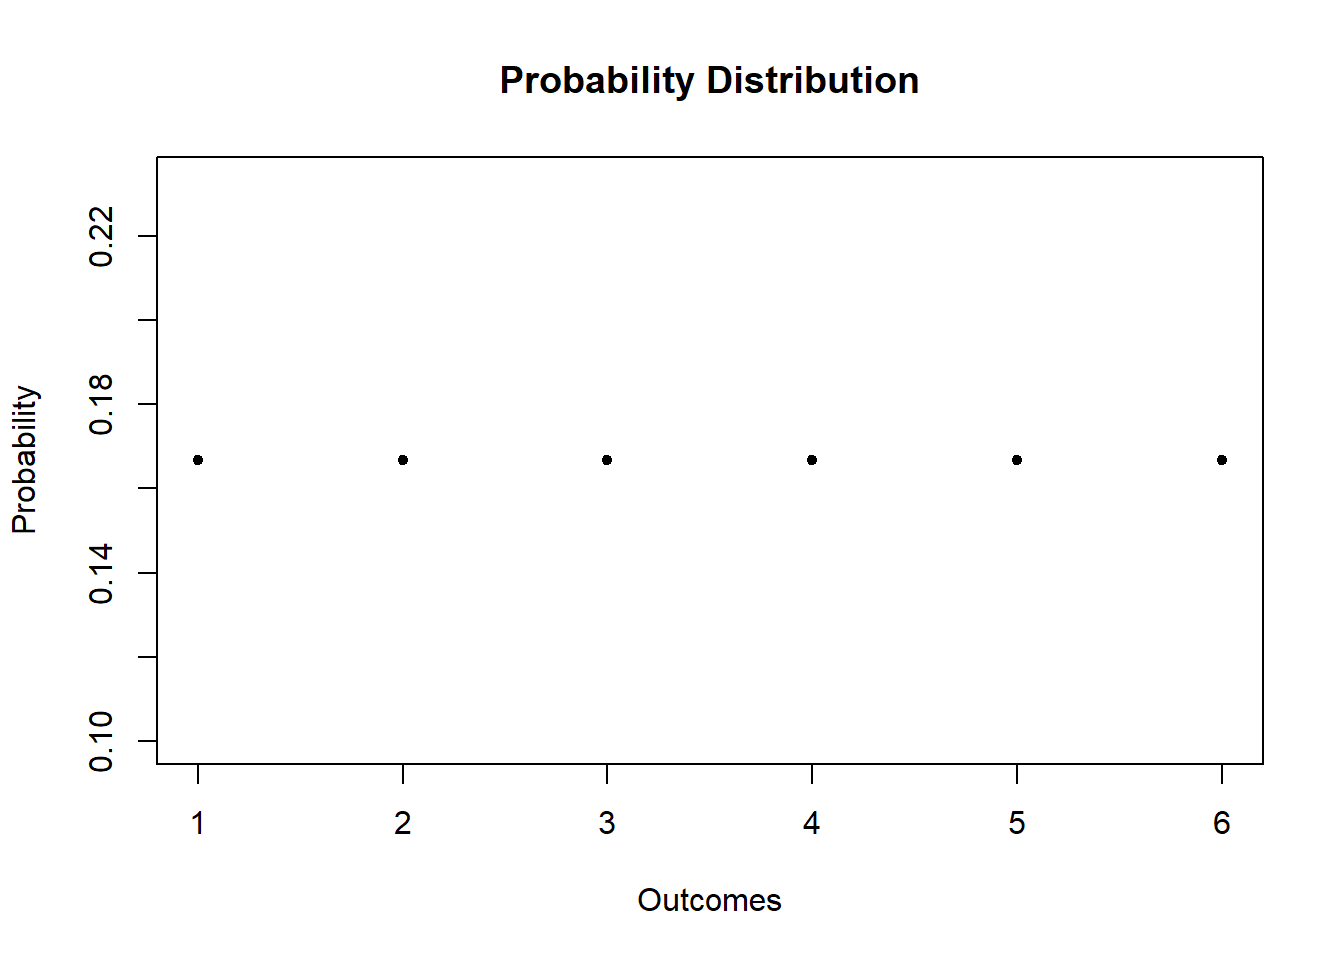
\includegraphics[width=0.8\linewidth]{06-ch6_files/figure-latex/unnamed-chunk-15-1} 

}

\caption{Visualisasi Dendogram}\label{fig:unnamed-chunk-15}
\end{figure}

\chapter{Visualisasi Dendogram}\label{vizhc}

Dendrogram merupakan representasi grafis yang menunjukkan bagaimana objek-objek dalam dataset dikelompokkan berdasarkan kemiripan atau jarak antar objek. Dalam dendrogram, setiap objek awalnya dianggap sebagai klaster terpisah. Proses penggabungan klaster dilakukan secara iteratif berdasarkan jarak terdekat hingga semua objek tergabung dalam satu klaster besar.

\section{Proses Pembentukan Dendrogram}\label{proses-pembentukan-dendrogram}

\begin{enumerate}
\def\labelenumi{\arabic{enumi}.}
\item
  Pengukuran Jarak: Langkah pertama adalah mengukur jarak antar objek menggunakan metode tertentu (misalnya, Euclidean distance).
\item
  Penggabungan Klaster: Klaster dengan jarak terdekat akan digabungkan menjadi satu klaster baru. Proses ini diulang hingga semua objek tergabung dalam satu klaster.
\item
  Pemotongan Dendrogram: Untuk menentukan jumlah klaster yang diinginkan, dendrogram dapat dipotong pada tingkat tertentu. Pemotongan ini membantu dalam mengidentifikasi kelompok-kelompok yang relevan dalam data
\end{enumerate}

\section{Eksperimen}\label{eksperimen}

\subsection*{Read Data}\label{read-data}
\addcontentsline{toc}{subsection}{Read Data}

\begin{Shaded}
\begin{Highlighting}[]
\FunctionTok{library}\NormalTok{ (readr)}
\NormalTok{urlfile }\OtherTok{=} \StringTok{"https://bit.ly/3VO3kRE"}
\NormalTok{data}\OtherTok{\textless{}{-}}\FunctionTok{read.csv}\NormalTok{(}\FunctionTok{url}\NormalTok{(urlfile), }\AttributeTok{row.names =} \StringTok{"Kabupaten"}\NormalTok{)}
\end{Highlighting}
\end{Shaded}

\begin{table}

\caption{\label{tab:nice-tab-2}Basis Data Terpadu Jawa Tengah}
\centering
\begin{tabular}[t]{lrrrrrrrrrr}
\toprule
  & X1 & X2 & X3 & X4 & X5 & X6 & X7 & X8 & X9 & X10\\
\midrule
CILACAP & 5.19 & 5.67 & 5.08 & 5.44 & 5.22 & 6.05 & 11.47 & 9.78 & 5.55 & 5.12\\
BANYUMAS & 5.71 & 4.47 & 5.18 & 5.51 & 5.02 & 6.21 & 7.39 & 6.96 & 5.98 & 8.22\\
PURBALINGGA & 3.30 & 2.19 & 3.80 & 3.13 & 3.73 & 3.34 & 8.71 & 7.41 & 3.21 & 4.65\\
BANJARNEGARA & 2.73 & 2.34 & 3.76 & 2.80 & 2.57 & 2.99 & 3.31 & 5.45 & 4.21 & 6.05\\
KEBUMEN & 4.17 & 2.55 & 3.26 & 4.16 & 3.15 & 4.15 & 4.30 & 9.29 & 4.61 & 4.34\\
\addlinespace
PURWOREJO & 1.87 & 2.12 & 1.48 & 3.05 & 1.78 & 1.83 & 5.00 & 4.90 & 3.12 & 2.09\\
WONOSOBO & 2.13 & 1.95 & 3.00 & 1.78 & 1.62 & 2.06 & 0.45 & 2.32 & 3.57 & 0.84\\
MAGELANG & 3.95 & 3.01 & 4.22 & 4.15 & 3.01 & 3.64 & 1.44 & 3.35 & 5.69 & 3.67\\
BOYOLALI & 2.19 & 3.07 & 1.61 & 2.74 & 2.11 & 1.82 & 1.71 & 2.34 & 3.41 & 1.55\\
KLATEN & 3.84 & 5.15 & 1.93 & 4.64 & 4.04 & 3.78 & 8.71 & 4.45 & 3.99 & 3.09\\
\bottomrule
\end{tabular}
\end{table}

\subsection*{Standarisasi Data}\label{standarisasi-data-1}
\addcontentsline{toc}{subsection}{Standarisasi Data}

Pertama, kita menghitung jarak antar kabupaten menggunakan fungsi \texttt{dist()}. Dalam hal ini, kita menggunakan metode jarak Euclidean. Sebelum menghitung jarak, data dinormalisasi dengan fungsi \texttt{scale()}, yang memastikan bahwa setiap variabel memiliki rata-rata 0 dan deviasi standar 1. Normalisasi ini penting untuk menghindari bias yang mungkin disebabkan oleh skala variabel yang berbeda.

\begin{Shaded}
\begin{Highlighting}[]
\NormalTok{data\_scale }\OtherTok{\textless{}{-}} \FunctionTok{dist}\NormalTok{(}\FunctionTok{scale}\NormalTok{(data), }\AttributeTok{method =} \StringTok{"euclidean"}\NormalTok{)}
\end{Highlighting}
\end{Shaded}

\subsection*{Pengelompokan Data}\label{pengelompokan-data}
\addcontentsline{toc}{subsection}{Pengelompokan Data}

Setelah menghitung jarak, langkah selanjutnya adalah melakukan pengelompokan menggunakan metode hirarki dengan fungsi \texttt{hclust()}. Dalam hal ini, kita menggunakan metode \texttt{Ward.D2}, yang bertujuan untuk meminimalkan varians dalam setiap kluster yang terbentuk. Metode ini sangat efektif dalam menghasilkan kluster yang lebih homogen.

\begin{Shaded}
\begin{Highlighting}[]
\NormalTok{hasil\_cluster }\OtherTok{\textless{}{-}} \FunctionTok{hclust}\NormalTok{(data\_scale, }\AttributeTok{method =} \StringTok{"ward.D2"}\NormalTok{)}
\end{Highlighting}
\end{Shaded}

\subsection*{Visualisasi Dendogram}\label{visualisasi-dendogram}
\addcontentsline{toc}{subsection}{Visualisasi Dendogram}

Visualisasi dendogram adalah alat penting dalam analisis kluster hirarki, yang memungkinkan kita untuk memahami struktur dan hubungan antar kelompok dalam data. Dalam konteks ini, kita menggunakan paket R \texttt{factoextra} dan \texttt{dendextend} untuk menghasilkan dan memodifikasi dendogram dari hasil analisis kluster. Kita dapat menggunakan fungsi \textbf{\texttt{fviz\_dend()}} dari paket \textbf{\texttt{factoextra}} di R untuk membuat dendrogram dengan mudah, baik menggunakan plot bawaan R atau melalui \textbf{\texttt{ggplot2}}.

Dalam analisis kluster hirarki, visualisasi dendogram adalah alat yang sangat berguna untuk memahami struktur dan hubungan antar objek dalam dataset. Dalam contoh ini, kita menggunakan fungsi \texttt{fviz\_dend()} untuk menghasilkan dendogram berdasarkan hasil klustering yang dilakukan dengan metode Ward.D2.

\begin{Shaded}
\begin{Highlighting}[]
\FunctionTok{library}\NormalTok{(factoextra)}
\FunctionTok{fviz\_dend}\NormalTok{(hasil\_cluster, }\AttributeTok{cex =} \FloatTok{0.5}\NormalTok{,}
        \AttributeTok{main =} \StringTok{"Dendrogram {-} ward.D2"}\NormalTok{,}
        \AttributeTok{xlab =} \StringTok{"Objects"}\NormalTok{, }\AttributeTok{ylab =} \StringTok{"Distance"}\NormalTok{, }\AttributeTok{sub =} \StringTok{""}\NormalTok{)}
\end{Highlighting}
\end{Shaded}

\begin{figure}[h]

{\centering \includegraphics[width=0.8\linewidth]{07-ch7_files/figure-latex/unnamed-chunk-4-1} 

}

\caption{Visualisasi Dendogram}\label{fig:unnamed-chunk-4}
\end{figure}

Untuk membuat visualisasi dendrogram dengan orientasi horizontal.

\begin{Shaded}
\begin{Highlighting}[]
\FunctionTok{fviz\_dend}\NormalTok{(hasil\_cluster, }\AttributeTok{cex =} \FloatTok{0.5}\NormalTok{, }\AttributeTok{horiz =} \ConstantTok{TRUE}\NormalTok{)}
\end{Highlighting}
\end{Shaded}

\begin{figure}[h]

{\centering \includegraphics[width=0.8\linewidth]{07-ch7_files/figure-latex/unnamed-chunk-5-1} 

}

\caption{Visualisasi Dendogram Horisontal}\label{fig:unnamed-chunk-5}
\end{figure}

Pohon dendrogram dapat dipotong pada ketinggian tertentu untuk membagi data menjadi beberapa kelompok. Dalam hal ini, cabang dapat diberi warna sesuai dengan kelompoknya, dan kotak dapat ditambahkan untuk menyoroti setiap kelompok. Kode ini digunakan untuk membuat dendrogram dengan pemotongan menjadi empat kelompok, memberikan warna pada cabang dan label berdasarkan kelompok, serta menambahkan kotak di sekitar setiap kelompok.

Untuk memberikan warna yang berbeda pada masing-masing kelompok dalam dendrogram, dapat dilakukan dengan menggunakan parameter \texttt{k\_colors} pada fungsi \texttt{fviz\_dend} dari paket \textbf{factoextra}. Parameter ini memungkinkan pengguna untuk menentukan warna yang akan digunakan untuk setiap klaster. Misalnya, pada kode berikut, dendrogram dipotong menjadi empat kelompok (\texttt{k\ =\ 4}), dan masing-masing kelompok diberi warna spesifik: biru (\#2E9FDF), hijau (\#00AFBB), kuning (\#E7B800), dan oranye (\#FC4E07). Selain itu, parameter \texttt{color\_labels\_by\_k\ =\ TRUE} memastikan bahwa label pada dendrogram juga diberi warna sesuai dengan kelompoknya, sehingga visualisasi menjadi lebih informatif dan mudah untuk diinterpretasikan.

\begin{Shaded}
\begin{Highlighting}[]
\FunctionTok{fviz\_dend}\NormalTok{(hasil\_cluster, }
          \AttributeTok{k =} \DecValTok{4}\NormalTok{,}
          \AttributeTok{cex =} \FloatTok{0.5}\NormalTok{, }
          \AttributeTok{k\_colors =} \FunctionTok{c}\NormalTok{(}\StringTok{"\#2E9FDF"}\NormalTok{, }\StringTok{"\#00AFBB"}\NormalTok{, }\StringTok{"\#E7B800"}\NormalTok{, }\StringTok{"\#FC4E07"}\NormalTok{), }
          \AttributeTok{color\_labels\_by\_k =} \ConstantTok{TRUE}\NormalTok{)}
\end{Highlighting}
\end{Shaded}

\begin{figure}[h]

{\centering \includegraphics[width=0.8\linewidth]{07-ch7_files/figure-latex/unnamed-chunk-6-1} 

}

\caption{Visualisasi Dendogram 4 Kelompok}\label{fig:unnamed-chunk-6}
\end{figure}

Parameter \texttt{k\_colors} dapat menggunakan berbagai palet warna, termasuk palet dari paket \textbf{RColorBrewer} (contoh: ``RdBu'', ``Blues'', ``Dark2'', ``Set2'', dan sebagainya) serta palet warna bertema jurnal ilmiah yang tersedia di paket \textbf{ggsci} (contoh: ``npg'', ``aaas'', ``lancet'', ``jco'', ``ucscgb'', ``uchicago'', ``simpsons'', dan ``rickandmorty'').

\begin{Shaded}
\begin{Highlighting}[]
\FunctionTok{fviz\_dend}\NormalTok{(hasil\_cluster, }\AttributeTok{cex =} \FloatTok{0.5}\NormalTok{, }\AttributeTok{k=}\DecValTok{4}\NormalTok{,}
\AttributeTok{k\_colors =} \StringTok{"jco"}\NormalTok{)}
\end{Highlighting}
\end{Shaded}

\begin{figure}[h]

{\centering \includegraphics[width=0.8\linewidth]{07-ch7_files/figure-latex/unnamed-chunk-7-1} 

}

\caption{Visualisasi Dendogram}\label{fig:unnamed-chunk-7}
\end{figure}

Kode ini digunakan untuk memvisualisasikan dendrogram hasil analisis klaster hierarkis dengan memotongnya menjadi empat kelompok (\texttt{k\ =\ 4}). Visualisasi dilakukan secara vertikal (\texttt{horiz\ =\ FALSE}), dengan ukuran label yang lebih kecil (\texttt{cex\ =\ 0.4}) untuk meningkatkan keterbacaan. Warna klaster dan batas persegi yang mengelilingi kelompok diatur menggunakan palet ``jco'' dari paket \textbf{ggsci} (\texttt{k\_colors\ =\ "jco"} dan \texttt{rect\_border\ =\ "jco"}). Persegi yang mengelilingi setiap klaster juga diisi dengan warna kelompok masing-masing (\texttt{rect\_fill\ =\ TRUE}). Hasilnya adalah dendrogram yang estetis dan mudah diinterpretasikan, dengan kelompok-kelompok yang ditampilkan secara jelas dan terorganisasi.

\begin{Shaded}
\begin{Highlighting}[]
\FunctionTok{fviz\_dend}\NormalTok{(hasil\_cluster, }\AttributeTok{k=}\DecValTok{4}\NormalTok{, }\AttributeTok{cex =} \FloatTok{0.4}\NormalTok{, }\AttributeTok{horiz =} \ConstantTok{FALSE}\NormalTok{, }\AttributeTok{k\_colors =} \StringTok{"jco"}\NormalTok{,}
\AttributeTok{rect =} \ConstantTok{TRUE}\NormalTok{, }\AttributeTok{rect\_border =} \StringTok{"jco"}\NormalTok{, }\AttributeTok{rect\_fill =} \ConstantTok{TRUE}\NormalTok{)}
\end{Highlighting}
\end{Shaded}

\begin{figure}[h]

{\centering \includegraphics[width=0.8\linewidth]{07-ch7_files/figure-latex/unnamed-chunk-8-1} 

}

\caption{Visualisasi Dendogram}\label{fig:unnamed-chunk-8}
\end{figure}

Kode ini digunakan untuk memvisualisasikan dendrogram hasil analisis klaster hierarkis dalam bentuk melingkar (\texttt{type\ =\ "circular"}). Dendrogram dipotong menjadi empat kelompok (\texttt{k\ =\ 4}), dan setiap klaster diberi warna menggunakan palet ``jco'' dari paket \textbf{ggsci} (\texttt{k\_colors\ =\ "jco"}). Ukuran label pada dendrogram diatur menjadi lebih kecil (\texttt{cex\ =\ 0.5}) untuk memastikan keterbacaan. Dengan bentuk melingkar, visualisasi ini memberikan tampilan yang estetis dan inovatif untuk analisis klaster, mempermudah identifikasi hubungan antar-objek dalam klaster.

\begin{Shaded}
\begin{Highlighting}[]
\FunctionTok{fviz\_dend}\NormalTok{(hasil\_cluster, }\AttributeTok{cex =} \FloatTok{0.5}\NormalTok{, }\AttributeTok{k=}\DecValTok{4}\NormalTok{,}
\AttributeTok{k\_colors =} \StringTok{"jco"}\NormalTok{, }\AttributeTok{type =} \StringTok{"circular"}\NormalTok{)}
\end{Highlighting}
\end{Shaded}

\begin{figure}[h]

{\centering \includegraphics[width=0.8\linewidth]{07-ch7_files/figure-latex/unnamed-chunk-9-1} 

}

\caption{Visualisasi Dendogram Bentuk Melingkar}\label{fig:unnamed-chunk-9}
\end{figure}

Kode ini digunakan untuk memvisualisasikan dendrogram hasil analisis klaster hierarkis dalam bentuk pohon filogenetik (\texttt{type\ =\ "phylogenic"}) menggunakan fungsi \texttt{fviz\_dend} dari paket \textbf{factoextra}. Dendrogram dipotong menjadi empat klaster (\texttt{k\ =\ 4}), dan setiap klaster diberi warna menggunakan palet ``jco'' dari paket \textbf{ggsci} (\texttt{k\_colors\ =\ "jco"}).

Parameter \texttt{repel\ =\ TRUE} digunakan untuk mengatur posisi label agar tidak saling bertumpukan, sehingga meningkatkan keterbacaan visualisasi. Paket \textbf{igraph} diperlukan untuk mendukung visualisasi pohon filogenetik ini. Hasil akhirnya adalah dendrogram yang menyerupai struktur pohon, cocok untuk menganalisis hubungan hierarkis dengan tampilan yang rapi dan informatif.

\begin{Shaded}
\begin{Highlighting}[]
\FunctionTok{require}\NormalTok{(}\StringTok{"igraph"}\NormalTok{)}
\FunctionTok{fviz\_dend}\NormalTok{(hasil\_cluster, }\AttributeTok{k=}\DecValTok{4}\NormalTok{, }\AttributeTok{k\_colors =} \StringTok{"jco"}\NormalTok{,}
\AttributeTok{type =} \StringTok{"phylogenic"}\NormalTok{, }\AttributeTok{repel =} \ConstantTok{TRUE}\NormalTok{)}
\end{Highlighting}
\end{Shaded}

\begin{figure}[h]

{\centering \includegraphics[width=0.8\linewidth]{07-ch7_files/figure-latex/unnamed-chunk-10-1} 

}

\caption{Visualisasi Dendogram Bentuk Filogenetik}\label{fig:unnamed-chunk-10}
\end{figure}

Kode ini digunakan untuk memvisualisasikan dendrogram hasil analisis klaster dan mengekstrak data dendrogram untuk pemrosesan lebih lanjut. Pertama, dendrogram divisualisasikan dengan memotongnya menjadi empat kelompok (\texttt{k\ =\ 4}) dan menggunakan palet warna ``jco'' untuk setiap klaster. Ukuran label ditentukan sebesar 0.5 (\texttt{cex\ =\ 0.5}).

Selanjutnya, data dendrogram diekstrak dari objek plot menggunakan \texttt{attr(dend\_plot,\ "dendrogram")}. Kemudian, dendrogram dipotong pada ketinggian tertentu (\texttt{h\ =\ 10}) dengan menggunakan fungsi \texttt{cut()}, yang menghasilkan dua cabang utama.

Terakhir, visualisasi dilakukan pada bagian atas dendrogram yang telah dipotong dengan menampilkan hanya cabang-cabang tersebut menggunakan \texttt{fviz\_dend(dend\_cuts\$upper)}. Hasilnya adalah dendrogram yang lebih sederhana, menampilkan dua cabang utama berdasarkan pemotongan pada ketinggian tertentu.

\begin{Shaded}
\begin{Highlighting}[]
\NormalTok{dend\_plot }\OtherTok{\textless{}{-}} \FunctionTok{fviz\_dend}\NormalTok{(hasil\_cluster, }\AttributeTok{k=}\DecValTok{4}\NormalTok{,}
\AttributeTok{cex =} \FloatTok{0.5}\NormalTok{,}
\AttributeTok{k\_colors =} \StringTok{"jco"}
\NormalTok{)}
\NormalTok{dend\_data }\OtherTok{\textless{}{-}} \FunctionTok{attr}\NormalTok{(dend\_plot, }\StringTok{"dendrogram"}\NormalTok{) }

\NormalTok{dend\_cuts }\OtherTok{\textless{}{-}} \FunctionTok{cut}\NormalTok{(dend\_data, }\AttributeTok{h=}\DecValTok{10}\NormalTok{)}

\FunctionTok{fviz\_dend}\NormalTok{(dend\_cuts}\SpecialCharTok{$}\NormalTok{upper)}
\end{Highlighting}
\end{Shaded}

\begin{center}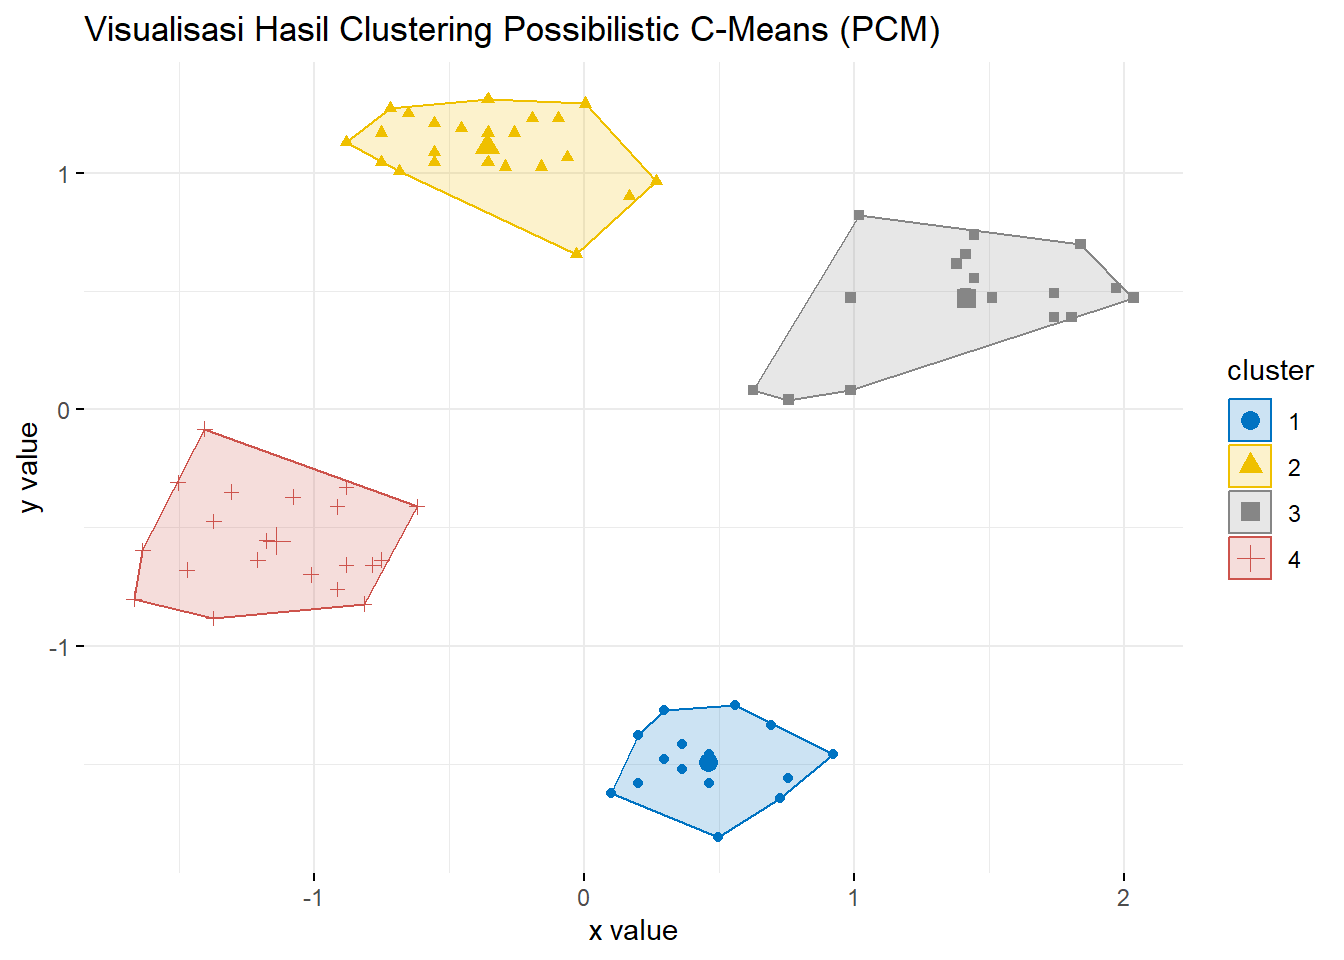
\includegraphics[width=0.8\linewidth]{07-ch7_files/figure-latex/unnamed-chunk-11-1} \end{center}

Kode ini digunakan untuk menampilkan dendrogram secara keseluruhan yang telah disiapkan sebelumnya. Dengan menggunakan \texttt{print(dend\_plot)}, visualisasi dendrogram yang telah dihasilkan oleh fungsi \texttt{fviz\_dend} akan ditampilkan. Dendrogram ini menunjukkan hasil klasterisasi dengan empat kelompok (\texttt{k\ =\ 4}) dan diberi warna berdasarkan palet ``jco'', dengan ukuran label yang diatur menjadi 0.5 (\texttt{cex\ =\ 0.5}).

\begin{Shaded}
\begin{Highlighting}[]
\FunctionTok{print}\NormalTok{(dend\_plot)}
\end{Highlighting}
\end{Shaded}

\begin{figure}[h]

{\centering \includegraphics[width=0.8\linewidth]{07-ch7_files/figure-latex/unnamed-chunk-12-1} 

}

\caption{Visualisasi Dendogram}\label{fig:unnamed-chunk-12}
\end{figure}

Kode ini digunakan untuk memvisualisasikan salah satu cabang bawah dari dendrogram yang telah dipotong sebelumnya. Dengan menggunakan \texttt{fviz\_dend(dend\_cuts\$lower{[}{[}1{]}{]},\ main\ =\ "Subtree\ 1")}, visualisasi akan menampilkan cabang pertama dari bagian bawah dendrogram yang telah dipotong pada ketinggian \texttt{h\ =\ 10}. Judul ``Subtree 1'' akan ditambahkan untuk menandai bagian ini, memudahkan interpretasi bagian tertentu dari hasil klasterisasi.

\begin{Shaded}
\begin{Highlighting}[]
\CommentTok{\# Plot subtree 1}
\FunctionTok{fviz\_dend}\NormalTok{(dend\_cuts}\SpecialCharTok{$}\NormalTok{lower[[}\DecValTok{1}\NormalTok{]], }\AttributeTok{main =} \StringTok{"Subtree 1"}\NormalTok{)}
\end{Highlighting}
\end{Shaded}

\begin{figure}[h]

{\centering \includegraphics[width=0.8\linewidth]{07-ch7_files/figure-latex/unnamed-chunk-13-1} 

}

\caption{Visualisasi Dendogram Subtree 1}\label{fig:unnamed-chunk-13}
\end{figure}

Kode ini digunakan untuk memvisualisasikan cabang kedua dari dendrogram yang telah dipotong sebelumnya. Dengan menggunakan \texttt{fviz\_dend(dend\_cuts\$lower{[}{[}2{]}{]},\ main\ =\ "Subtree\ 2")}, visualisasi akan menampilkan cabang kedua dari bagian bawah dendrogram yang telah dipotong pada ketinggian \texttt{h\ =\ 10}. Judul ``Subtree 2'' akan ditambahkan untuk mempermudah identifikasi bagian ini, sehingga hasil klasterisasi dapat dianalisis dengan lebih detail pada cabang kedua tersebut.

\begin{Shaded}
\begin{Highlighting}[]
\CommentTok{\# Plot subtree 2}
\FunctionTok{fviz\_dend}\NormalTok{(dend\_cuts}\SpecialCharTok{$}\NormalTok{lower[[}\DecValTok{2}\NormalTok{]], }\AttributeTok{main =} \StringTok{"Subtree 2"}\NormalTok{)}
\end{Highlighting}
\end{Shaded}

\begin{figure}[h]

{\centering \includegraphics[width=0.8\linewidth]{07-ch7_files/figure-latex/unnamed-chunk-14-1} 

}

\caption{Visualisasi Dendogram Subtree 2}\label{fig:unnamed-chunk-14}
\end{figure}

\part{Pendekatan Fuzzy}\label{part-pendekatan-fuzzy}

\chapter{Algoritma Fuzzy C-Means}\label{fcm}

Algoritma fuzzy c-means (FCM) merupakan salah satu metode clustering yang banyak digunakan dalam analisis data dan pengolahan citra. Berbeda dengan algoritma clustering tradisional seperti k-means, yang mengelompokkan data ke dalam cluster yang jelas dan tegas, FCM memberikan fleksibilitas dengan memungkinkan setiap data untuk memiliki derajat keanggotaan pada lebih dari satu cluster. Hal ini menjadikan FCM sangat berguna dalam situasi di mana batasan antara cluster tidak dapat ditentukan dengan jelas \citep{bezdek1981pattern}.

FCM pertama kali diperkenalkan oleh Bezdek pada tahun 1981 dan sejak saat itu telah banyak diterapkan dalam berbagai bidang, termasuk pengolahan citra, pengenalan pola, dan analisis data multidimensi. Metode ini bekerja dengan meminimalkan fungsi objektif yang mengukur kesalahan antara data dan pusat cluster, dengan mempertimbangkan derajat keanggotaan setiap data terhadap cluster yang ada. Proses ini dilakukan secara iteratif hingga konvergensi tercapai, di mana perubahan pusat cluster dan derajat keanggotaan menjadi sangat kecil \citep{dunn1973fuzzy}.

Salah satu keunggulan FCM adalah kemampuannya untuk menangani data yang memiliki noise atau outlier. Dalam banyak aplikasi dunia nyata, data sering kali tidak bersih dan mengandung kesalahan pengukuran. Dengan menggunakan derajat keanggotaan, FCM dapat mengurangi pengaruh data yang tidak representatif terhadap hasil clustering, sehingga menghasilkan model yang lebih robust dan akurat \citep{pal1995cluster}.

Namun, meskipun FCM memiliki banyak kelebihan, algoritma ini juga memiliki beberapa kelemahan. Salah satunya adalah ketergantungan pada pemilihan jumlah cluster yang tepat, yang dapat mempengaruhi hasil akhir. Selain itu, FCM juga dapat menjadi sensitif terhadap inisialisasi pusat cluster, yang dapat menyebabkan hasil yang berbeda pada setiap iterasi \citep{huang1998extensions}. Oleh karena itu, penelitian lebih lanjut diperlukan untuk mengembangkan metode yang dapat mengatasi masalah ini.

Dalam konteks perkembangan teknologi dan kebutuhan analisis data yang semakin kompleks, FCM tetap menjadi salah satu metode yang relevan dan banyak digunakan. Penelitian dan pengembangan lebih lanjut dalam algoritma ini diharapkan dapat meningkatkan kinerjanya dan memperluas aplikasinya di berbagai bidang, termasuk kecerdasan buatan dan analisis big data. Dengan demikian, pemahaman yang mendalam tentang FCM dan aplikasinya sangat penting bagi para peneliti dan praktisi di bidang ini.

Klastering dengan algoritma Fuzzy C-Means didasarkan pada teori logika fuzzy yang diperkenalkan oleh Lotfi Zadeh pada tahun 1965 dengan nama himpunan fuzzy (fuzzy set). Fuzzy C-Means Clustering pertama kali diperkenalkan oleh Dun pada (1973) dan diperbaiki oleh Bezdek \citep{bezdek1981pattern} . Dalam teori fuzzy, keangotaan sebuah data diberikan dengan suatu nilai derajat keanggotaan yang jangkauan nilainya 0 sampai 1. Semakin tinggi nilai derajat keanggotaannya maka semakin tinggi nilai keanggotaan sebuah data dalam suatu kelompok dan semakin kecil nilai derajat keanggotaannya maka semakin rendah nilai keanggotaan sebuah data dalam suatu kelompok.

\section{Tahapan Algoritma Fuzzy C-Means}\label{tahapan-algoritma-fuzzy-c-means}

\subsection*{1. Inisialisasi Parameter}\label{inisialisasi-parameter}
\addcontentsline{toc}{subsection}{1. Inisialisasi Parameter}

Tentukan jumlah cluster (\emph{c}), parameter pembobot (\emph{m}, biasanya \(m > 1\)), toleransi error (\(\epsilon\)), dan maksimum iterasi.

\subsection*{2. Inisialisasi Matriks Keanggotaan}\label{inisialisasi-matriks-keanggotaan}
\addcontentsline{toc}{subsection}{2. Inisialisasi Matriks Keanggotaan}

Buat matriks keanggotaan awal (\(U^{(0)}\)) secara acak. Matriks ini memiliki ukuran \(N \times c\), di mana \(N\) adalah jumlah data, dan \(c\) adalah jumlah cluster. Pastikan bahwa \(\sum_{j=1}^c u_{ij} = 1\) untuk setiap data \(i\).

\subsection*{3. Perhitungan Pusat Cluster}\label{perhitungan-pusat-cluster}
\addcontentsline{toc}{subsection}{3. Perhitungan Pusat Cluster}

Hitung pusat cluster (\(v_k\)) untuk setiap cluster \(k\) menggunakan rumus:
\[
     v_k = \frac{\sum_{i=1}^N u_{ik}^m x_i}{\sum_{i=1}^N u_{ik}^m}
     \]
di mana \(u_{ik}\) adalah nilai keanggotaan data \(i\) pada cluster \(k\) dan \(x_i\) adalah data ke-\(i\).

\subsection*{4. Perbarui Matriks Keanggotaan}\label{perbarui-matriks-keanggotaan}
\addcontentsline{toc}{subsection}{4. Perbarui Matriks Keanggotaan}

Hitung matriks keanggotaan baru (\(U^{(t+1)}\)) dengan rumus:
\[
     u_{ik} = \frac{1}{\sum_{j=1}^c \left( \frac{\|x_i - v_k\|}{\|x_i - v_j\|} \right)^{\frac{2}{m-1}}}
     \]
di mana \(\|x_i - v_k\|\) adalah jarak antara data \(i\) dan pusat cluster \(k\).

\subsection*{5. Evaluasi Konvergensi}\label{evaluasi-konvergensi}
\addcontentsline{toc}{subsection}{5. Evaluasi Konvergensi}

Hitung perubahan matriks keanggotaan (\(\|U^{(t+1)} - U^{(t)}\|\)).
Jika perubahan lebih kecil dari toleransi error (\(\epsilon\)) atau iterasi maksimum tercapai, algoritma berhenti. Jika tidak, kembali ke langkah 3.

\subsection*{6. Hasil Akhir}\label{hasil-akhir-2}
\addcontentsline{toc}{subsection}{6. Hasil Akhir}

Pusat cluster (\(v_k\)) dan matriks keanggotaan (\(u_{ik}\)) akhir menunjukkan distribusi data terhadap cluster. Data dapat diklasifikasikan ke cluster dengan keanggotaan tertinggi.

\section{Eksperimeen Fuzzy C-Means}\label{eksperimeen-fuzzy-c-means}

\subsection*{Install dan Load Packagaes}\label{install-dan-load-packagaes}
\addcontentsline{toc}{subsection}{Install dan Load Packagaes}

Untuk memulai eksperimen menggunakan algoritma Fuzzy C-Means (FCM) di \texttt{R}, beberapa library perlu diinstal dan dimuat untuk mendukung proses analisis, visualisasi, dan validasi hasil clustering. Library \texttt{ppclust} menyediakan berbagai metode clustering berbasis partisi, termasuk FCM, dan berfungsi untuk mengimplementasikan algoritma serta mengevaluasi hasil clustering. Library \texttt{factoextra} digunakan untuk memudahkan visualisasi hasil clustering, seperti menampilkan scatter plot dengan pembagian cluster yang jelas. Selain itu, library \texttt{fclust} mendukung berbagai fungsi terkait clustering berbasis fuzzy, termasuk penghitungan indeks validasi untuk menilai kualitas cluster. Terakhir, library \texttt{cluster} menawarkan berbagai alat untuk clustering dan validasi, termasuk perbandingan hasil clustering FCM dengan algoritma lain seperti K-Means atau PAM.

\begin{Shaded}
\begin{Highlighting}[]
\FunctionTok{library}\NormalTok{(ppclust)}
\FunctionTok{library}\NormalTok{(factoextra)}
\FunctionTok{library}\NormalTok{(fclust)}
\FunctionTok{library}\NormalTok{(cluster)}
\end{Highlighting}
\end{Shaded}

\subsection*{Data}\label{data-2}
\addcontentsline{toc}{subsection}{Data}

Dataset diimpor ke dalam \texttt{R} menggunakan library \texttt{readr}, yang dirancang untuk membaca data dengan format seperti CSV secara efisien. Data diakses melalui URL \texttt{https://bit.ly/3VO3kRE} dan dimuat menggunakan fungsi \texttt{read.csv()}. Parameter \texttt{row.names\ =\ "Kabupaten"} digunakan untuk menjadikan kolom ``Kabupaten'' sebagai indeks baris, sehingga setiap baris data dapat diidentifikasi berdasarkan nama kabupaten. Setelah proses ini, dataset disimpan dalam variabel \texttt{data} sebagai sebuah \emph{data frame}, yang siap digunakan untuk analisis lebih lanjut, seperti preprocessing, penerapan algoritma clustering, atau visualisasi hasil.

\begin{Shaded}
\begin{Highlighting}[]
\FunctionTok{library}\NormalTok{ (readr)}
\NormalTok{urlfile }\OtherTok{=} \StringTok{"https://bit.ly/3VO3kRE"}
\NormalTok{data}\OtherTok{\textless{}{-}}\FunctionTok{read.csv}\NormalTok{(}\FunctionTok{url}\NormalTok{(urlfile), }\AttributeTok{row.names =} \StringTok{"Kabupaten"}\NormalTok{)}
\end{Highlighting}
\end{Shaded}

\begin{table}

\caption{\label{tab:nice-tab-1}Basis Data Terpadu Jawa Tengah}
\centering
\begin{tabular}[t]{lrrrrrrrrrr}
\toprule
  & X1 & X2 & X3 & X4 & X5 & X6 & X7 & X8 & X9 & X10\\
\midrule
CILACAP & 5.19 & 5.67 & 5.08 & 5.44 & 5.22 & 6.05 & 11.47 & 9.78 & 5.55 & 5.12\\
BANYUMAS & 5.71 & 4.47 & 5.18 & 5.51 & 5.02 & 6.21 & 7.39 & 6.96 & 5.98 & 8.22\\
PURBALINGGA & 3.30 & 2.19 & 3.80 & 3.13 & 3.73 & 3.34 & 8.71 & 7.41 & 3.21 & 4.65\\
BANJARNEGARA & 2.73 & 2.34 & 3.76 & 2.80 & 2.57 & 2.99 & 3.31 & 5.45 & 4.21 & 6.05\\
KEBUMEN & 4.17 & 2.55 & 3.26 & 4.16 & 3.15 & 4.15 & 4.30 & 9.29 & 4.61 & 4.34\\
\addlinespace
PURWOREJO & 1.87 & 2.12 & 1.48 & 3.05 & 1.78 & 1.83 & 5.00 & 4.90 & 3.12 & 2.09\\
WONOSOBO & 2.13 & 1.95 & 3.00 & 1.78 & 1.62 & 2.06 & 0.45 & 2.32 & 3.57 & 0.84\\
MAGELANG & 3.95 & 3.01 & 4.22 & 4.15 & 3.01 & 3.64 & 1.44 & 3.35 & 5.69 & 3.67\\
BOYOLALI & 2.19 & 3.07 & 1.61 & 2.74 & 2.11 & 1.82 & 1.71 & 2.34 & 3.41 & 1.55\\
KLATEN & 3.84 & 5.15 & 1.93 & 4.64 & 4.04 & 3.78 & 8.71 & 4.45 & 3.99 & 3.09\\
\bottomrule
\end{tabular}
\end{table}

\subsection*{Hasil Clustering}\label{hasil-clustering}
\addcontentsline{toc}{subsection}{Hasil Clustering}

Hasil clustering diperoleh dengan menerapkan algoritma Fuzzy C-Means (FCM) menggunakan fungsi \texttt{fcm()} dari library \texttt{ppclust}. Dataset yang telah dipersiapkan dianalisis untuk menghasilkan tiga pusat cluster dengan parameter \texttt{centers=3}. Setelah proses clustering selesai, nilai derajat keanggotaan masing-masing data terhadap setiap cluster disimpan dalam matriks keanggotaan (\(u\)). Matriks ini kemudian dikonversi menjadi format \emph{data frame} menggunakan fungsi \texttt{as.data.frame()} agar lebih mudah diakses dan dianalisis. Setiap baris dalam \emph{data frame} merepresentasikan satu data observasi, sementara kolom-kolomnya menunjukkan derajat keanggotaan terhadap masing-masing cluster. Derajat keanggotaan ini mencerminkan probabilitas relatif atau tingkat afiliasi suatu data terhadap cluster tertentu.

\begin{Shaded}
\begin{Highlighting}[]
\FunctionTok{library}\NormalTok{(ppclust)}
\NormalTok{res.fcm }\OtherTok{\textless{}{-}} \FunctionTok{fcm}\NormalTok{(data, }\AttributeTok{centers=}\DecValTok{3}\NormalTok{)}
\FunctionTok{as.data.frame}\NormalTok{(res.fcm}\SpecialCharTok{$}\NormalTok{u)}
\CommentTok{\#\textgreater{}                  Cluster 1  Cluster 2  Cluster 3}
\CommentTok{\#\textgreater{} CILACAP         0.09432155 0.70608174 0.19959671}
\CommentTok{\#\textgreater{} BANYUMAS        0.03242738 0.87685700 0.09071562}
\CommentTok{\#\textgreater{} PURBALINGGA     0.12503329 0.58855259 0.28641412}
\CommentTok{\#\textgreater{} BANJARNEGARA    0.15770912 0.27431153 0.56797934}
\CommentTok{\#\textgreater{} KEBUMEN         0.12183017 0.55326811 0.32490172}
\CommentTok{\#\textgreater{} PURWOREJO       0.37665821 0.15508384 0.46825795}
\CommentTok{\#\textgreater{} WONOSOBO        0.73997169 0.04794255 0.21208577}
\CommentTok{\#\textgreater{} MAGELANG        0.12565978 0.11864932 0.75569090}
\CommentTok{\#\textgreater{} BOYOLALI        0.65917928 0.04746322 0.29335751}
\CommentTok{\#\textgreater{} KLATEN          0.15366683 0.40625017 0.44008300}
\CommentTok{\#\textgreater{} SUKOHARJO       0.90659203 0.01812578 0.07528219}
\CommentTok{\#\textgreater{} WONOGIRI        0.62649398 0.05984340 0.31366262}
\CommentTok{\#\textgreater{} KARANGANYAR     0.83280963 0.03151333 0.13567704}
\CommentTok{\#\textgreater{} SRAGEN          0.92987167 0.01369224 0.05643609}
\CommentTok{\#\textgreater{} GROBOGAN        0.10906165 0.20509357 0.68584478}
\CommentTok{\#\textgreater{} BLORA           0.42364979 0.06584083 0.51050938}
\CommentTok{\#\textgreater{} REMBANG         0.77496097 0.03515460 0.18988443}
\CommentTok{\#\textgreater{} PATI            0.18226626 0.18018760 0.63754615}
\CommentTok{\#\textgreater{} KUDUS           0.93999864 0.01358093 0.04642043}
\CommentTok{\#\textgreater{} JEPARA          0.13357477 0.17434136 0.69208387}
\CommentTok{\#\textgreater{} DEMAK           0.22405973 0.12077163 0.65516864}
\CommentTok{\#\textgreater{} SEMARANG        0.92443899 0.01375558 0.06180543}
\CommentTok{\#\textgreater{} TEMANGGUNG      0.92181846 0.01515432 0.06302723}
\CommentTok{\#\textgreater{} KENDAL          0.30783534 0.07103512 0.62112953}
\CommentTok{\#\textgreater{} BATANG          0.74568211 0.05146780 0.20285008}
\CommentTok{\#\textgreater{} PEKALONGAN      0.33879435 0.11753007 0.54367557}
\CommentTok{\#\textgreater{} PEMALANG        0.13508254 0.47108349 0.39383397}
\CommentTok{\#\textgreater{} TEGAL           0.08391671 0.61445746 0.30162583}
\CommentTok{\#\textgreater{} BREBES          0.11958050 0.64100931 0.23941019}
\CommentTok{\#\textgreater{} KOTA MAGELANG   0.82227544 0.05127744 0.12644712}
\CommentTok{\#\textgreater{} KOTA SURAKARTA  0.88284897 0.03051218 0.08663885}
\CommentTok{\#\textgreater{} KOTA SALATIGA   0.82356236 0.05093432 0.12550332}
\CommentTok{\#\textgreater{} KOTA SEMARANG   0.81177689 0.04152177 0.14670134}
\CommentTok{\#\textgreater{} KOTA PEKALONGAN 0.87988142 0.03226874 0.08784985}
\CommentTok{\#\textgreater{} KOTA TEGAL      0.88100104 0.03188749 0.08711147}
\end{Highlighting}
\end{Shaded}

\subsection*{Visualisasi Matrik Keanggotaan}\label{visualisasi-matrik-keanggotaan}
\addcontentsline{toc}{subsection}{Visualisasi Matrik Keanggotaan}

Untuk memvisualisasikan matriks keanggotaan yang dihasilkan oleh algoritma Fuzzy C-Means (FCM) menggunakan fungsi \texttt{corrplot()} dari library \texttt{corrplot}. Matriks keanggotaan yang terdapat dalam \texttt{res.fcm\$u} menggambarkan derajat keanggotaan masing-masing data terhadap setiap cluster. Dengan parameter \texttt{is.corr\ =\ FALSE}, kita memberi tahu fungsi bahwa data yang akan divisualisasikan bukanlah matriks korelasi, melainkan matriks keanggotaan FCM. Visualisasi ini membantu untuk memahami bagaimana data tersebar di antara cluster dan seberapa kuat hubungan data dengan setiap cluster berdasarkan derajat keanggotaannya. Grafik ini dapat memperlihatkan pola atau struktur dalam data yang terkelompok dengan cara yang lebih mudah dipahami.

\begin{Shaded}
\begin{Highlighting}[]
\CommentTok{\# Visualize using corrplot}
\FunctionTok{library}\NormalTok{(corrplot)}
\FunctionTok{corrplot}\NormalTok{(res.fcm}\SpecialCharTok{$}\NormalTok{u, }\AttributeTok{is.corr =} \ConstantTok{FALSE}\NormalTok{)}
\end{Highlighting}
\end{Shaded}

\begin{figure}[h]

{\centering \includegraphics[width=0.8\linewidth]{08-ch8_files/figure-latex/unnamed-chunk-4-1} 

}

\caption{Matrik Keagotaan}\label{fig:unnamed-chunk-4}
\end{figure}

Kode ini digunakan untuk mengakses dan menampilkan pusat cluster pertama (\(v_0\)) yang dihasilkan oleh algoritma Fuzzy C-Means (FCM) yang telah diterapkan pada dataset. Pada objek \texttt{res.fcm}, atribut \texttt{v0} menyimpan informasi tentang pusat cluster pada iterasi pertama. Nilai ini menunjukkan posisi awal dari setiap cluster sebelum algoritma mulai melakukan iterasi lebih lanjut untuk memperbarui posisi pusat cluster berdasarkan derajat keanggotaan data. Dengan menampilkan \texttt{res.fcm\$v0}, kita dapat melihat posisi awal cluster dalam ruang fitur data dan mengevaluasi bagaimana posisi tersebut berfungsi dalam pemisahan data pada iterasi selanjutnya.

\begin{Shaded}
\begin{Highlighting}[]
\NormalTok{res.fcm}\SpecialCharTok{$}\NormalTok{v0}
\CommentTok{\#\textgreater{}             X1   X2    X3   X4   X5   X6    X7   X8   X9   X10}
\CommentTok{\#\textgreater{} Cluster 1 2.19 3.07  1.61 2.74 2.11 1.82  1.71 2.34 3.41  1.55}
\CommentTok{\#\textgreater{} Cluster 2 5.19 5.67  5.08 5.44 5.22 6.05 11.47 9.78 5.55  5.12}
\CommentTok{\#\textgreater{} Cluster 3 7.45 4.26 10.94 5.13 4.99 8.17  5.61 7.11 3.97 11.40}
\end{Highlighting}
\end{Shaded}

Kode ini digunakan untuk mengakses dan menampilkan pusat cluster yang dihasilkan setelah algoritma Fuzzy C-Means (FCM) selesai dijalankan. Pada objek \texttt{res.fcm}, atribut \texttt{v} menyimpan informasi tentang posisi pusat cluster yang telah diperbarui setelah iterasi terakhir. Pusat cluster ini merupakan hasil akhir dari proses clustering dan menunjukkan lokasi sentroid (pusat) dari setiap cluster berdasarkan data dan derajat keanggotaan yang telah dihitung. Dengan menampilkan \texttt{res.fcm\$v}, kita dapat melihat posisi akhir setiap cluster dalam ruang fitur data, yang membantu untuk memahami bagaimana data telah dikelompokkan ke dalam cluster yang berbeda setelah proses clustering selesai.

\begin{Shaded}
\begin{Highlighting}[]
\NormalTok{res.fcm}\SpecialCharTok{$}\NormalTok{v}
\CommentTok{\#\textgreater{}                 X1       X2       X3       X4       X5       X6       X7}
\CommentTok{\#\textgreater{} Cluster 1 1.724771 1.743303 1.432408 1.706002 1.626688 1.504833 1.335312}
\CommentTok{\#\textgreater{} Cluster 2 5.001721 4.041093 5.531054 4.669414 4.638562 5.500335 6.458007}
\CommentTok{\#\textgreater{} Cluster 3 3.418238 4.025821 3.497306 3.657048 3.843888 3.477061 3.074419}
\CommentTok{\#\textgreater{}                 X8       X9      X10}
\CommentTok{\#\textgreater{} Cluster 1 1.021470 1.697120 1.056498}
\CommentTok{\#\textgreater{} Cluster 2 7.009924 4.458629 6.474407}
\CommentTok{\#\textgreater{} Cluster 3 3.057133 3.802309 3.529256}
\end{Highlighting}
\end{Shaded}

\subsection*{Ringkasan Hasil Clustering FCM}\label{ringkasan-hasil-clustering-fcm}
\addcontentsline{toc}{subsection}{Ringkasan Hasil Clustering FCM}

Untuk menampilkan ringkasan dari hasil algoritma Fuzzy C-Means (FCM) yang telah dijalankan, menggunakan fungsi \texttt{summary()} pada objek \texttt{res.fcm}. Fungsi ini memberikan gambaran umum tentang hasil clustering, termasuk informasi mengenai pusat cluster, derajat keanggotaan, dan konvergensi algoritma. Biasanya, hasil yang ditampilkan mencakup jumlah cluster yang terbentuk, posisi pusat cluster akhir, serta statistik terkait keanggotaan data terhadap cluster. Dengan menggunakan \texttt{summary(res.fcm)}, kita dapat memperoleh insight terkait seberapa baik algoritma telah mengelompokkan data dan apakah proses clustering telah konvergen, serta informasi tambahan yang dapat membantu evaluasi kualitas clustering.

\begin{Shaded}
\begin{Highlighting}[]
\FunctionTok{summary}\NormalTok{(res.fcm)}
\CommentTok{\#\textgreater{} Summary for \textquotesingle{}res.fcm\textquotesingle{}}
\CommentTok{\#\textgreater{} }
\CommentTok{\#\textgreater{} Number of data objects:  35 }
\CommentTok{\#\textgreater{} }
\CommentTok{\#\textgreater{} Number of clusters:  3 }
\CommentTok{\#\textgreater{} }
\CommentTok{\#\textgreater{} Crisp clustering vector:}
\CommentTok{\#\textgreater{}  [1] 2 2 2 3 2 3 1 3 1 3 1 1 1 1 3 3 1 3 1 3 3 1 1 3 1 3 2 2 2 1 1 1 1 1 1}
\CommentTok{\#\textgreater{} }
\CommentTok{\#\textgreater{} Initial cluster prototypes:}
\CommentTok{\#\textgreater{}             X1   X2    X3   X4   X5   X6    X7   X8   X9   X10}
\CommentTok{\#\textgreater{} Cluster 1 2.19 3.07  1.61 2.74 2.11 1.82  1.71 2.34 3.41  1.55}
\CommentTok{\#\textgreater{} Cluster 2 5.19 5.67  5.08 5.44 5.22 6.05 11.47 9.78 5.55  5.12}
\CommentTok{\#\textgreater{} Cluster 3 7.45 4.26 10.94 5.13 4.99 8.17  5.61 7.11 3.97 11.40}
\CommentTok{\#\textgreater{} }
\CommentTok{\#\textgreater{} Final cluster prototypes:}
\CommentTok{\#\textgreater{}                 X1       X2       X3       X4       X5       X6       X7}
\CommentTok{\#\textgreater{} Cluster 1 1.724771 1.743303 1.432408 1.706002 1.626688 1.504833 1.335312}
\CommentTok{\#\textgreater{} Cluster 2 5.001721 4.041093 5.531054 4.669414 4.638562 5.500335 6.458007}
\CommentTok{\#\textgreater{} Cluster 3 3.418238 4.025821 3.497306 3.657048 3.843888 3.477061 3.074419}
\CommentTok{\#\textgreater{}                 X8       X9      X10}
\CommentTok{\#\textgreater{} Cluster 1 1.021470 1.697120 1.056498}
\CommentTok{\#\textgreater{} Cluster 2 7.009924 4.458629 6.474407}
\CommentTok{\#\textgreater{} Cluster 3 3.057133 3.802309 3.529256}
\CommentTok{\#\textgreater{} }
\CommentTok{\#\textgreater{} Distance between the final cluster prototypes}
\CommentTok{\#\textgreater{}           Cluster 1 Cluster 2}
\CommentTok{\#\textgreater{} Cluster 2 165.71763          }
\CommentTok{\#\textgreater{} Cluster 3  42.66853  48.57171}
\CommentTok{\#\textgreater{} }
\CommentTok{\#\textgreater{} Difference between the initial and final cluster prototypes}
\CommentTok{\#\textgreater{}                   X1        X2         X3         X4         X5         X6}
\CommentTok{\#\textgreater{} Cluster 1 {-}0.4652294 {-}1.326697 {-}0.1775916 {-}1.0339977 {-}0.4833119 {-}0.3151670}
\CommentTok{\#\textgreater{} Cluster 2 {-}0.1882786 {-}1.628907  0.4510540 {-}0.7705855 {-}0.5814383 {-}0.5496647}
\CommentTok{\#\textgreater{} Cluster 3 {-}4.0317618 {-}0.234179 {-}7.4426942 {-}1.4729516 {-}1.1461115 {-}4.6929386}
\CommentTok{\#\textgreater{}                  X7        X8         X9        X10}
\CommentTok{\#\textgreater{} Cluster 1 {-}0.374688 {-}1.318530 {-}1.7128795 {-}0.4935021}
\CommentTok{\#\textgreater{} Cluster 2 {-}5.011993 {-}2.770076 {-}1.0913711  1.3544068}
\CommentTok{\#\textgreater{} Cluster 3 {-}2.535581 {-}4.052867 {-}0.1676907 {-}7.8707443}
\CommentTok{\#\textgreater{} }
\CommentTok{\#\textgreater{} Root Mean Squared Deviations (RMSD): 8.764585 }
\CommentTok{\#\textgreater{} Mean Absolute Deviation (MAD): 185.823 }
\CommentTok{\#\textgreater{} }
\CommentTok{\#\textgreater{} Membership degrees matrix (top and bottom 5 rows): }
\CommentTok{\#\textgreater{}               Cluster 1 Cluster 2  Cluster 3}
\CommentTok{\#\textgreater{} CILACAP      0.09432155 0.7060817 0.19959671}
\CommentTok{\#\textgreater{} BANYUMAS     0.03242738 0.8768570 0.09071562}
\CommentTok{\#\textgreater{} PURBALINGGA  0.12503329 0.5885526 0.28641412}
\CommentTok{\#\textgreater{} BANJARNEGARA 0.15770912 0.2743115 0.56797934}
\CommentTok{\#\textgreater{} KEBUMEN      0.12183017 0.5532681 0.32490172}
\CommentTok{\#\textgreater{} ...}
\CommentTok{\#\textgreater{}                 Cluster 1  Cluster 2  Cluster 3}
\CommentTok{\#\textgreater{} KOTA SURAKARTA  0.8828490 0.03051218 0.08663885}
\CommentTok{\#\textgreater{} KOTA SALATIGA   0.8235624 0.05093432 0.12550332}
\CommentTok{\#\textgreater{} KOTA SEMARANG   0.8117769 0.04152177 0.14670134}
\CommentTok{\#\textgreater{} KOTA PEKALONGAN 0.8798814 0.03226873 0.08784985}
\CommentTok{\#\textgreater{} KOTA TEGAL      0.8810010 0.03188749 0.08711147}
\CommentTok{\#\textgreater{} }
\CommentTok{\#\textgreater{} Descriptive statistics for the membership degrees by clusters}
\CommentTok{\#\textgreater{}           Size       Min        Q1      Mean    Median        Q3       Max}
\CommentTok{\#\textgreater{} Cluster 1   17 0.6264940 0.7749610 0.8295979 0.8328096 0.9065920 0.9399986}
\CommentTok{\#\textgreater{} Cluster 2    7 0.4710835 0.5709104 0.6359014 0.6144575 0.6735455 0.8768570}
\CommentTok{\#\textgreater{} Cluster 3   11 0.4400830 0.5270925 0.5979972 0.6211295 0.6705067 0.7556909}
\CommentTok{\#\textgreater{} }
\CommentTok{\#\textgreater{} Dunn\textquotesingle{}s Fuzziness Coefficients:}
\CommentTok{\#\textgreater{} dunn\_coeff normalized }
\CommentTok{\#\textgreater{}  0.5999684  0.3999525 }
\CommentTok{\#\textgreater{} }
\CommentTok{\#\textgreater{} Within cluster sum of squares by cluster:}
\CommentTok{\#\textgreater{}        1        2        3 }
\CommentTok{\#\textgreater{} 130.5953 220.3251 200.0818 }
\CommentTok{\#\textgreater{} (between\_SS / total\_SS =  61.98\%) }
\CommentTok{\#\textgreater{} }
\CommentTok{\#\textgreater{} Available components: }
\CommentTok{\#\textgreater{}  [1] "u"          "v"          "v0"         "d"          "x"         }
\CommentTok{\#\textgreater{}  [6] "cluster"    "csize"      "sumsqrs"    "k"          "m"         }
\CommentTok{\#\textgreater{} [11] "iter"       "best.start" "func.val"   "comp.time"  "inpargs"   }
\CommentTok{\#\textgreater{} [16] "algorithm"  "call"}
\end{Highlighting}
\end{Shaded}

Menjalankan algoritma Fuzzy C-Means (FCM) pada dataset \texttt{data} dengan jumlah cluster yang ditentukan sebanyak 3 (\texttt{centers=3}) dan parameter \texttt{nstart=5}. Parameter \texttt{nstart=5} menunjukkan bahwa algoritma FCM akan dijalankan sebanyak 5 kali dengan inisialisasi pusat cluster yang berbeda pada setiap iterasi. Tujuan dari parameter ini adalah untuk meningkatkan kemungkinan menemukan solusi yang lebih baik dengan memulai algoritma dari berbagai kondisi awal, sehingga mengurangi kemungkinan terjebak pada solusi lokal yang tidak optimal. Setelah proses ini, hasil clustering akan disimpan dalam objek \texttt{res.fcm}, yang dapat digunakan untuk mengevaluasi pusat cluster, derajat keanggotaan, dan validitas clustering.

\begin{Shaded}
\begin{Highlighting}[]
\NormalTok{res.fcm }\OtherTok{\textless{}{-}} \FunctionTok{fcm}\NormalTok{(data, }\AttributeTok{centers=}\DecValTok{3}\NormalTok{, }\AttributeTok{nstart=}\DecValTok{5}\NormalTok{)}
\end{Highlighting}
\end{Shaded}

Untuk menampilkan nilai objektif (fungsi tujuan) dari hasil terbaik yang ditemukan selama eksperimen Fuzzy C-Means (FCM). Nilai ini dapat diakses melalui \texttt{res.fcm\$func.val}, yang memberikan informasi tentang nilai minimum dari fungsi tujuan (objective function) pada iterasi terakhir setelah algoritma selesai dijalankan.

Fungsi tujuan dalam FCM biasanya mengukur sejauh mana data sesuai dengan pusat cluster yang telah dihitung, dengan mempertimbangkan derajat keanggotaan data terhadap setiap cluster. Semakin rendah nilai fungsi tujuan, semakin baik hasil clustering yang dihasilkan, karena itu menunjukkan pemisahan yang lebih baik antara cluster dan data. Dengan menampilkan \texttt{res.fcm\$func.val}, kita dapat mengevaluasi kualitas solusi terbaik yang ditemukan, yang sering digunakan sebagai indikator untuk memvalidasi hasil clustering yang diperoleh dengan multiple starts.

\begin{Shaded}
\begin{Highlighting}[]
\NormalTok{res.fcm}\SpecialCharTok{$}\NormalTok{func.val}
\CommentTok{\#\textgreater{} [1] 360.931 360.931 360.931 360.931 360.931}
\end{Highlighting}
\end{Shaded}

Untuk menampilkan jumlah iterasi yang dibutuhkan oleh algoritma Fuzzy C-Means (FCM) untuk mencapai konvergensi. Atribut \texttt{res.fcm\$iter} menyimpan informasi tentang jumlah iterasi yang dilakukan selama proses clustering hingga algoritma mencapai kondisi konvergen, yaitu saat perubahan posisi pusat cluster atau matriks keanggotaan menjadi sangat kecil atau mencapai batas iterasi maksimum.

Menampilkan \texttt{res.fcm\$iter} memberikan wawasan tentang seberapa cepat atau lambat algoritma FCM mencapai konvergensi dalam eksperimen yang dijalankan. Jumlah iterasi yang rendah menunjukkan bahwa algoritma dengan cepat menemukan solusi yang stabil, sementara jumlah iterasi yang tinggi dapat menunjukkan bahwa proses clustering membutuhkan waktu lebih lama untuk mencapai hasil yang konvergen.

\begin{Shaded}
\begin{Highlighting}[]
\NormalTok{res.fcm}\SpecialCharTok{$}\NormalTok{iter}
\CommentTok{\#\textgreater{} [1] 79 76 75 82 61}
\end{Highlighting}
\end{Shaded}

Untuk menampilkan hasil terbaik dari beberapa percobaan yang dilakukan selama eksekusi algoritma Fuzzy C-Means (FCM) dengan multiple starts. Atribut \texttt{res.fcm\$best.start} menunjukkan indeks dari percobaan (start) yang menghasilkan solusi terbaik berdasarkan nilai fungsi tujuan (objective function) terendah.

Selama penggunaan \texttt{nstart}, algoritma FCM dijalankan beberapa kali dengan inisialisasi pusat cluster yang berbeda. \texttt{res.fcm\$best.start} memberikan informasi tentang percobaan yang memberikan hasil terbaik, yang berarti percobaan tersebut memiliki nilai fungsi tujuan yang lebih kecil dibandingkan dengan percobaan lainnya. Ini membantu untuk mengetahui solusi yang paling optimal yang ditemukan oleh algoritma setelah menjalankan beberapa percobaan.

\begin{Shaded}
\begin{Highlighting}[]
\NormalTok{res.fcm}\SpecialCharTok{$}\NormalTok{best.start}
\CommentTok{\#\textgreater{} [1] 1}
\end{Highlighting}
\end{Shaded}

\subsection*{Visualisasi Hasil Cluster}\label{visualisasi-hasil-cluster-1}
\addcontentsline{toc}{subsection}{Visualisasi Hasil Cluster}

Untuk memvisualisasikan hasil clustering yang diperoleh dari algoritma Fuzzy C-Means (FCM) menggunakan fungsi \texttt{fviz\_cluster()} dari paket \texttt{factoextra}. Pertama, hasil clustering FCM yang disimpan dalam objek \texttt{res.fcm} diubah menjadi format yang kompatibel dengan visualisasi menggunakan fungsi \texttt{ppclust2()}. Hasil clustering kemudian diproses untuk diperlakukan seperti hasil dari algoritma K-Means. Selanjutnya, fungsi \texttt{fviz\_cluster()} digunakan untuk memplot hasil clustering, dengan parameter tambahan seperti \texttt{ellipse.type\ =\ "convex"} untuk menambahkan elips konveks yang menggambarkan area setiap cluster, dan \texttt{palette\ =\ "jco"} untuk memberikan warna berbeda pada setiap cluster. Selain itu, \texttt{repel\ =\ TRUE} memastikan label titik data tidak saling tumpang tindih, sehingga grafik menjadi lebih mudah dibaca. Visualisasi ini memberikan gambaran yang jelas tentang pemisahan data ke dalam cluster yang berbeda, memudahkan analisis hasil clustering dan memahami struktur data.

\begin{Shaded}
\begin{Highlighting}[]
\NormalTok{res.fcm2 }\OtherTok{\textless{}{-}} \FunctionTok{ppclust2}\NormalTok{(res.fcm, }\StringTok{"kmeans"}\NormalTok{)}
\NormalTok{factoextra}\SpecialCharTok{::}\FunctionTok{fviz\_cluster}\NormalTok{(res.fcm2, }\AttributeTok{data =}\NormalTok{ data, }
  \AttributeTok{ellipse.type =} \StringTok{"convex"}\NormalTok{,}
  \AttributeTok{palette =} \StringTok{"jco"}\NormalTok{,}
  \AttributeTok{repel =} \ConstantTok{TRUE}\NormalTok{)}
\end{Highlighting}
\end{Shaded}

\begin{figure}[h]

{\centering \includegraphics[width=0.8\linewidth]{08-ch8_files/figure-latex/unnamed-chunk-12-1} 

}

\caption{Hasil Clustering FCM}\label{fig:unnamed-chunk-12}
\end{figure}

\subsection*{Visualisasi Hasil Cluster dengan clusplot}\label{visualisasi-hasil-cluster-dengan-clusplot}
\addcontentsline{toc}{subsection}{Visualisasi Hasil Cluster dengan clusplot}

Kode ini digunakan untuk memvisualisasikan hasil clustering Fuzzy C-Means (FCM) menggunakan fungsi \texttt{clusplot()} dari paket \texttt{cluster}. Pertama, hasil clustering yang disimpan dalam objek \texttt{res.fcm} diubah menjadi format yang kompatibel dengan algoritma fuzzy \texttt{fanny} menggunakan fungsi \texttt{ppclust2()}. Selanjutnya, fungsi \texttt{clusplot()} digunakan untuk memplot hasil clustering dalam ruang dua dimensi. Data yang digunakan untuk clustering distandarisasi terlebih dahulu dengan \texttt{scale()} untuk memastikan setiap fitur memiliki skala yang seragam. Hasil clustering yang diperoleh kemudian diplot, dengan setiap cluster diberi warna yang berbeda, dan label ditampilkan pada titik data sesuai dengan cluster mereka. Plot ini juga menyertakan garis pemisah antara cluster, sehingga memudahkan pemahaman tentang bagaimana data terkelompok dan sejauh mana pemisahan antara cluster tersebut. Visualisasi ini memberikan gambaran yang jelas tentang struktur data, yang sangat berguna dalam analisis hasil clustering FCM.

\begin{Shaded}
\begin{Highlighting}[]
\NormalTok{res.fcm3 }\OtherTok{\textless{}{-}} \FunctionTok{ppclust2}\NormalTok{(res.fcm, }\StringTok{"fanny"}\NormalTok{)}

\NormalTok{cluster}\SpecialCharTok{::}\FunctionTok{clusplot}\NormalTok{(}\FunctionTok{scale}\NormalTok{(data), res.fcm3}\SpecialCharTok{$}\NormalTok{cluster,  }
  \AttributeTok{main =} \StringTok{"Cluster plot of Iris data set"}\NormalTok{,}
  \AttributeTok{color=}\ConstantTok{TRUE}\NormalTok{, }\AttributeTok{labels =} \DecValTok{2}\NormalTok{, }\AttributeTok{lines =} \DecValTok{2}\NormalTok{, }\AttributeTok{cex=}\DecValTok{1}\NormalTok{)}
\end{Highlighting}
\end{Shaded}

\begin{figure}[h]

{\centering \includegraphics[width=0.8\linewidth]{08-ch8_files/figure-latex/unnamed-chunk-13-1} 

}

\caption{Visualisasi Hasil FCM dengan Clusplot}\label{fig:unnamed-chunk-13}
\end{figure}

\chapter*{Referensi}\label{References}
\addcontentsline{toc}{chapter}{Referensi}

  \bibliography{book.bib,packages.bib}

\end{document}
